\documentclass[11pt]{book}

\usepackage{tikz}
\usetikzlibrary{datavisualization}
\usetikzlibrary{calc}
\tikzset{/tikz/trim left=0} % Bounding box without the labels of the axis

\usepackage{amsmath}
\usepackage{amsfonts}
\usepackage{amssymb}
\usepackage{xfrac} % to use slanted fractions
\usepackage[bold-style=ISO]{unicode-math} % for bold math symbols

\usepackage{epsfig}
\usepackage{epic}
\usepackage{eepic}

%% For some reason I am not able to make the hyper links to work, so it should
%% be the case that I am missing something here.
\usepackage{hyperref}

\pdfpagewidth=\paperwidth
\pdfpageheight=\paperheight

% To change the fontsize of the captions
\usepackage[font=footnotesize]{caption}

% package `subfigure` and `subfig` are deprecated and should not be used
% unless withing the IEEETran or ACM SIG templates
\usepackage{subcaption}

% To have tables with stretching and accross several pages
\usepackage{tabu}

% To use more customizable footnotes
\usepackage[symbol]{footmisc}

% To handle the acronyms nicely
% - ucmark = true --> so that it sets the mark for the header to be upper case
% - nogroupskip --> so that it does not leave special separation between
%                   logical groups, I don't fully know what these are, but the
%                   result is that there were weird different separations in
%                   some of the lines.
% [See the manual of `glossaries` for more information
\usepackage[nonumberlist, toc, acronym, ucmark=true, nogroupskip]{glossaries}
\pagenumbering{gobble}
\newacronym{csma}{CSMA}{Carrier Sense Multiple Access}
\newacronym{fdd}{FDD}{Frequency Division Duplexing}
\newacronym{tdd}{TDD}{Time Division Duplexing}
\newacronym{fdma}{FDMA}{Frequency Division Multiple Access}
\newacronym{tdma}{TDMA}{Time Division Multiple Access}
\newacronym{cdma}{CDMA}{Code Division Multiple Access}
\newacronym{wcdma}{WCDMA}{Wide-band Code Division Multiple Access}
\newacronym{ss}{SS}{Spread Spectrum}
\newacronym{sdma}{SDMA}{Space Division Multiple Access}
\newacronym{sdm}{SDM}{Space Division Multiplexing}
\newacronym{ofdm}{OFDM}{Orthogonal Frequency Division Multiplexing}
\newacronym{ofdma}{OFDMA}{Orthogonal Frequency Division Multiple Access}
\newacronym{ufr}{UFR}{Universal Frequency Reuse}
\newacronym{5g}{5G}{5$^{th}$ Generation of Mobile Communications}
\newacronym{4g}{4G}{4$^{th}$ Generation of Mobile Communications}
\newacronym{3g}{3G}{3$^{rd}$ Generation of Mobile Communications}
\newacronym{3gpp}{3GPP}{3$^{rd}$ Generation Partnership Project}
\newacronym{hspa+}{HSPA+}{High-Speed Packet Access Plus}
\newacronym{lte}{LTE}{Long Term Evolution}
\newacronym{ltea}{LTE-A}{Long Term Evolution Advanced}
\newacronym{mimo}{MIMO}{Multiple Input Multiple Output}
\newacronym{mumimo}{MU-MIMO}{Multi User Multiple Input Multiple Output}
\newacronym{miso}{MISO}{Multiple Input Single Output}
\newacronym{siso}{SISO}{Single Input Single Output}
\newacronym{itu}{ITU}{International Telecommunication Union}
\newacronym{itur}{ITU-R}{International Telecommunication Union Radiocommunication Sector}
\newacronym{imta}{IMT-Advanced}{International Mobile Telecommunications\hyp{}Advanced}
\newacronym{ca}{CA}{Carrier Aggregation}
\newacronym{rn}{RN}{Relay Node}
\newacronym{comp}{CoMP}{Coordinated Multi Point}
\newacronym{zf}{ZF}{Zero Forcing}
\newacronym{bd}{BD}{Block Diagonalization}
\newacronym{mmse}{MMSE}{Minimum Mean Squared Error}
\newacronym{mse}{MSE}{Mean Squared Error}
\newacronym{qos}{QoS}{Quality of Service}
\newacronym{dpc}{DPC}{Dirty Paper Coding}
\newacronym{cbst}{CBST}{Coordinated Base Station Transmission}
\newacronym{ocelli}{OcI}{Out Cell Interference}
\newacronym{snr}{SNR}{Signal to Noise Ratio}
\newacronym{sir}{SIR}{Signal to Interference Ratio}
\newacronym{sinr}{SINR}{Signal to Interference plus Noise Ratio}
\newacronym{csi}{CSI}{Channel State Information}
\newacronym{svd}{SVD}{Singular Value Decomposition}
\newacronym{bs}{BS}{Base Station}
\newacronym{awgn}{AWGN}{Additive White Gaussian Noise}
\newacronym{papc}{PAPC}{Per Antenna Power Constraint}
\newacronym{pbpc}{PBPC}{Per Base Station Power Constraint}
\newacronym{tpc}{TPC}{Total Power Constraint}
\newacronym{kkt}{KKT}{Karush-Kuhn-Tucker}
\newacronym{iid}{iid}{independent identically distributed}
\newacronym{pdf}{pdf}{probability density function}
\newacronym{cdf}{CDF}{Cumulative Distribution Function}
\newacronym{oci}{OCI}{Other Cluster Interference}
\newacronym{su}{SU}{Single User}
\newacronym{mrt}{MRT}{Maximum Ratio Combining}
\newacronym{zfbf}{ZFBF}{Zero Forcing Beamforming}
\newacronym{hetnet}{HetNet}{Heterogeneous Networks}
\newacronym{bc}{BC}{Broadcast Channel}
\newacronym{mac}{MAC}{Multiple Access Channel}
\newacronym{ia}{IA}{Interference Alignment}
\newacronym{bia}{BIA}{Blind Interference Alignment}

\makeglossaries

% To handle left subscripts
\usepackage{tensor}

% To use URLs in the references and other parts of the document
\usepackage{url}

% algorithm typesetting
\usepackage{algorithm}
\usepackage{algpseudocode}

% For empty useless text, just to fill pages for the sake of doing it
\usepackage{lipsum}

% Renaming of some commands
\newcommand{\refc}[1]{Chapter~\ref{#1}}
\newcommand{\refa}[1]{Appendix~\ref{#1}}
\newcommand{\refs}[1]{Section~\ref{#1}}
\newcommand{\refss}[1]{Subsection~\ref{#1}}
\newcommand{\reff}[1]{Figure~\ref{#1}}
\newcommand{\refal}[1]{Algorithm~\ref{#1}}

% Margins
\usepackage[top=3.5cm, bottom=3.5cm, left=3.5cm, right=3.5cm]{geometry}

\setlength{\parskip}{1em plus0.2em minus0.2em}

% Include up to subsections in the TOC
\setcounter{tocdepth}{2}

% So that the empty pages have no page number
\makeatletter
  \def\cleardoublepage{\clearpage\if@twoside \ifodd\c@page\else
  \vspace*{\fill}
    \thispagestyle{empty}
    \newpage
    \if@twocolumn\hbox{}\newpage\fi\fi\fi}
\makeatother

% Definition of custom symbol commands
\def\tx{\text{tx}}
\def\rx{\text{rx}}
\def\db{\text{dB}}
\def\dee{\text{d}}

\def\C{\mathbb{C}}
\def\R{\mathbb{R}}

\def\Ltilde{\widetilde{L}}
\def\Lhat{\widehat{L}}
\def\lambdahat{\hat{\lambda}}
\def\lambdahatsqrt{\hat{\lambda}^{\sfrac{1}{2}}}

\def\Rcell{R_{\text{cell}}}
\def\Dtone{D_{\text{tier 1}}}
\def\Dtonebar{\overline{D}_{\text{tier 1}}}
\def\Dttwo{D_{\text{tier 2}}}
\def\Dttwobar{\overline{D}_{\text{tier 2}}}
\def\Minterf{M_{\text{interf}}}
\def\Meqi{M_{\text{eq},i}}
\def\Minti{M_{\text{int},i}}

\def\Np{N^{\prime}}

\def\hgeo{\tensor*[_2]{\text{F}}{_1}}

% Matrices
\def\zero{\mathbf{0}}
\def\eye{\mathbf{I}}

\def\HH{\mathbf{H}}
\def\Htilde{\mathbf{\widetilde{H}}}
\def\Hhat{\mathbf{\widehat{H}}}
\def\Hbar{\mathbf{\bar{H}}}

\def\WW{\mathbf{W}}
\def\Wtx{\mathbf{W}^{(\tx)}}
\def\WtxBar{\mathbf{\overline{W}}^{(\tx)}}
\def\WtxH{\mathbf{W}^{(\tx),H}}
\def\WtxHbar{\mathbf{\overline{W}}^{(\tx),H}}
\def\Wrx{\mathbf{W}^{(\rx)}}
\def\WrxH{\mathbf{W}^{(\rx),H}}

\def\UU{\mathbf{U}}
\def\Utilde{\mathbf{\widetilde{U}}}
\def\Uhat{\mathbf{\widehat{U}}}

\def\VV{\mathbf{V}}
\def\Vtilde{\mathbf{\widetilde{V}}}
\def\Vhat{\mathbf{\widehat{V}}}

\def\bSigma{\mathbf{\Sigma}}
\def\bSigmatilde{\mathbf{\widetilde{\Sigma}}}
\def\bSigmahat{\mathbf{\widehat{\Sigma}}}

\def\bLambda{\mathbf{\Lambda}}
\def\bLambdatilde{\mathbf{\widetilde{\Lambda}}}
\def\bLambdahat{\mathbf{\widehat{\Lambda}}}

\def\OmegaEq{\Omega_{ik}^{\text{BS}}}

\def\RR{\mathbf{R}}
\def\PP{\mathbf{P}}

\def\AA{\mathbf{A}}

\def\nablabf{\mathbf{\nabla}}

% Vectors
\def\yy{\mathbf{y}}
\def\xx{\mathbf{x}}
\def\ww{\mathbf{w}}
\def\wbar{\mathbf{\bar{w}}}
\def\nn{\mathbf{n}}
\def\ss{\mathbf{s}}
\def\zz{\mathbf{z}}
\def\pp{\mathbf{p}}
\def\aa{\mathbf{a}}

\DeclareMathOperator*{\Tr}{Tr}
\DeclareMathOperator*{\rank}{rank}
% \DeclareMathOperator*{\ker}{Ker} % surprise surprise, kernel operator already
                                   % defined
\DeclareMathOperator*{\diag}{diag}
\DeclareMathOperator*{\blkdiag}{blkdiag}
\DeclareMathOperator*{\maxi}{maximize}
\DeclareMathOperator*{\mini}{minimize}
\DeclareMathOperator*{\maxp}{max.}
\DeclareMathOperator*{\st}{subject\,to}
\DeclareMathOperator*{\stp}{s.t.}

% Dummy box for images to be placed later
\def\dummybox{\framebox(266.67, 150){}}

% original from Roberto's hand
\def\be{\begin{equation}}
\def\ee{\end{equation}}
\def\miH{\mathbf{H}}
\def\miy{\mathbf{y}}
\def\mix{\mathbf{x}}
\def\miw{\mathbf{w}}
\def\miW{\mathbf{W}}
\def\minn{\mathbf{n}}
\def\mib{\mathbf{b}}
\def\miT{\text{T}}
\def\miQ{\mathbf{Q}}
\def\miR{\mathbf{R}}
\def\mi0{\mathbf{0}}
\def\miI{\mathbf{I}}
\def\miU{\mathbf{U}}
\def\miS{\mathbf{S}}
\def\miSigma{\mathbf{\Sigma}}


% To use BibLaTeX
\usepackage[doi=false, % to hide the DOI field present in some entries
            isbn=false, % to hide the ISSN/ISBN field present in some entries
            style=ieee]{biblatex}
% File with references information
\addbibresource{./bibliography/references.bib}

% % To change the style of the pages
% \usepackage{fancyhdr}
% \pagestyle{fancy}

%%%%%%%%%%%%%%%%%%%%%%%%%%%%%%%%%%%%%%%%%%%%%%%%%%%%%%%%%%%%%%%%%%%%%%%%%%%%%%%%
\begin{document}

%%%%%%%%%%%%%%%%%%%%%%%%%%%%%%%%%%%%%%%%%%%%%%%%%%%%%%%%%%%%%%%%%%%%%%%%%%%%%%%%
% PREFACE

\frontmatter
\pagenumbering{gobble}
\cleardoublepage
\thispagestyle{plain}
{\Large
\centering

\vspace*{\fill}


\includegraphics[width=0.6\textwidth]{./00.foreword/img/logo_uc3m} 

\vspace*{2cm}

DOCTORAL THESIS

\vspace*{2cm}

{\bf
BLOCK DIAGONALIZATION TECHNIQUES FOR CELLULAR NETWORKS:
CLUSTERING AND SCHEDULING
}

\vspace*{2cm}

Author: JUAN JOSÉ GARCÍA FERNÁNDEZ

Advisor: ANA GARCÍA ARMADA

\vspace*{2cm}

Departamento de Teoría de la Señal y Comunicaciones

\vspace*{2cm}

Leganés, June 2015

\vspace*{\fill}

} % Large

\newpage

\cleardoublepage
\thispagestyle{plain}
\noindent
\begin{tabular}{l l}
{\bf Tesis Doctoral:} 
& BLOCK DIAGONALIZATION TECHNIQUES\\
& FOR CELLULAR NETWORKS:\\
& CLUSTERING AND SCHEDULING\\
\\
{\bf Autor:} 
& Juan José García Fernández\\
\\
{\bf Director:} 
& Dra. Ana García Armada
\\
\end{tabular}

\vspace*{2cm}

\noindent
El tribunal nombrado para juzgar la tesis doctoral arriba citada, compuesto por los doctores


\vspace*{1cm}

\noindent
Presidente:

\vspace*{2cm}

\noindent
Vocal:


\vspace*{2cm}

\noindent
Secretario:

\vspace{2cm}
\noindent
acuerda otorgarle la calificación de

\vspace{2cm}
\noindent
Leganés, a

\newpage

\cleardoublepage
% First part uses roman numbering
\pagenumbering{Roman}
\chapter*{Acknowledgements}
% {\Huge {\bf Acknowledgements}}

\lipsum[5]

\newpage

\cleardoublepage
\chapter*{Abstract}
% {\Huge {\bf Abstract}}

\lipsum[5]

\newpage

\cleardoublepage
{\Huge {\bf Resumen}}

\lipsum[5]

\newpage

% Index
\tableofcontents{}

% List of tables and Figures
% % \listoftables{} % Who wants tables?!
\listoffigures{}

% Notation page
\cleardoublepage
\chapter*{Notation}

{ % taller table rows
\renewcommand{\arraystretch}{1.5}

\begin{tabularx}{\textwidth}{lX}
$a$ & Scalar. \\
$\aa$ & Vector. \\
$\AA$ & Matrix. \\
$\AA^{-1}$ & Inverse of the matrix $\AA$. \\
$\AA^\dagger$ & Pseudo-inverse of the matrix $\AA$. \\
$\AA^T$ & Transpose of a matrix. \\
$\AA^\ast$ & Complex conjugate of a matrix. \\
$\AA^H$ & Transpose and complex conjugate of a matrix
    (Hermitian). \\
$\zero$ & Vector/matrix of zeros of the appropriate dimensions. \\
$\eye$ & Identity matrix of the appropriate dimensions. \\

$\Tr\left(\AA\right)$ & Trace of the matrix $\AA$. \\
$\left|\AA\right|$ & Determinant of the matrix $\AA$. \\
$\rank\left(\AA\right)$ & Rank of the matrix $\AA$. \\
$\ker\left(\AA\right)$ & Kernel/null-space of the matrix $\AA$. \\
$\blkdiag\left(\AA_1, \ldots, \AA_N\right)$ & Block diagonal matrix
    formed with the matrices $\left\{\AA_1, \ldots, \AA_N\right\}$. \\
$\diag\left(a_1, \ldots, a_N\right)$ & Diagonal matrix whose main
    diagonal is $\left\{a_1, \ldots, a_N\right\}$. \\
$\left\|\aa\right\|_2$ & Norm-2 (Euclidean norm) of the vector $\aa$, see
    \eqref{eq:norm2}. \\
$\nablabf_{\xx}f(\xx)$ & Gradient of a function $f(\xx)$,
    \eqref{eq:gradient} \\
$\mathbb{E}\left\{\cdot\right\}$ & Statistical expectation. \\
$\log\left(\cdot\right)$ & Natural (base $e$) logarithm. \\
$\log_2\left(\cdot\right)$ & Base 2 logarithm. \\
$\left[ a \right]^+$ & $\max\left( 0,a \right)$. \\
$\mathbb{R}$ & Field of real numbers. \\
$\mathbb{R}^+$ & Set of positive real numbers. \\
$\mathbb{R}^+ \cup \left\{0\right\}$ & Set of non-negative real numbers. \\
$\mathbb{C}$ & Field of complex numbers.
\end{tabularx}

}

\newpage

% Acronyms
\printglossary[type=\acronymtype]

\mainmatter

%%%%%%%%%%%%%%%%%%%%%%%%%%%%%%%%%%%%%%%%%%%%%%%%%%%%%%%%%%%%%%%%%%%%%%%%%%%%%%%%
% CHAPTERS

% Back to arabic numbering
\pagenumbering{arabic}

% Introduction
\chapter{Introduction}\label{ch:intro}

Every new generation of cellular network technologies comes with a new set of
requirements, dictated by the trends in the use of the mobile connectivity. A
common requirement to every single generation is their striving for higher data
rates and greater power efficiency. This motivates research and techology
innovation in order to achieve the goals set for each generation.


The research associated usually requires revisiting old paradigms used in
previous generations, and updating them with novel ideas.


The \emph{release 7} of the \gls{3gpp} \gls{3g} specifications \cite{3gpprel7},
also known as \gls{hspa+}, included the use of \gls{mimo} as a means to increase
the transmission rates.


\emph{Release 8}, more well known by its commercial name \gls{lte}
\cite{3gpplte}, introduced a new physical layer, based on \gls{ofdm} instead of
\gls{wcdma} as in \gls{3g}. Although the rates attainable with \gls{wcdma} may
be comparable to those obtained with \gls{ofdm}, the latter provides a much
easier equalization mechanism that makes dealing with multipath channels a
simpler task. Apart from that \gls{ofdm} provides a higher flexibility in the
resource allocation and user and enables the use of \gls{ofdma}.

\gls{lte} did not meet the requirements issued by the \gls{itur} \gls{imta}
radio interface \cite{imta} for what is known as \gls{4g} though.

The introduction of \gls{ltea} in \emph{release 10} of the LTE specification
\cite{3gppltea} met the requirements to be considered an \gls{imta} system. The
main novelties included in \gls{ltea} are \gls{ca}, enhanced use of MIMO
techniques and support for \glspl{rn}.

\emph{Release 11} \cite{3gpprel11} included in the specification the support for
\gls{comp} operation. \gls{comp} was included in order to improve the network
performance at cell edges, for it uses several transmitters to provide
coordinated transmission in the downlink, and a number of receivers to provide
coordinated reception in the uplink.

With \gls{ltea} standardized and its deployment already ongoing, further
releases of \gls{ltea} still continue but standards bodies and industry are
already looking ahead at the future \gls{5g}, and so is doing the research
world. Even though there is no definite idea about what \gls{5g} will be, it is 
clear what it will \emph{not} be, an incremental advance on \gls{4g}. It needs
to be a paradigm shift \cite{andrews14}.

The new \gls{5g} systems will be characterized by being heterogeneous, what is
known as \glspl{hetnet}, formed by multiple small cells, using different radio
access technologies \cite{chin14}. One of the main problems for \glspl{hetnet}
is inter-cell interference, because of the possible presence of unplanned
deployment of small cells, and the irregular shape of the cells. Hence the importance of interference coordination techniques.

\begin{figure}[t]
    \centering
    \begin{subfigure}[b]{0.45\textwidth}
            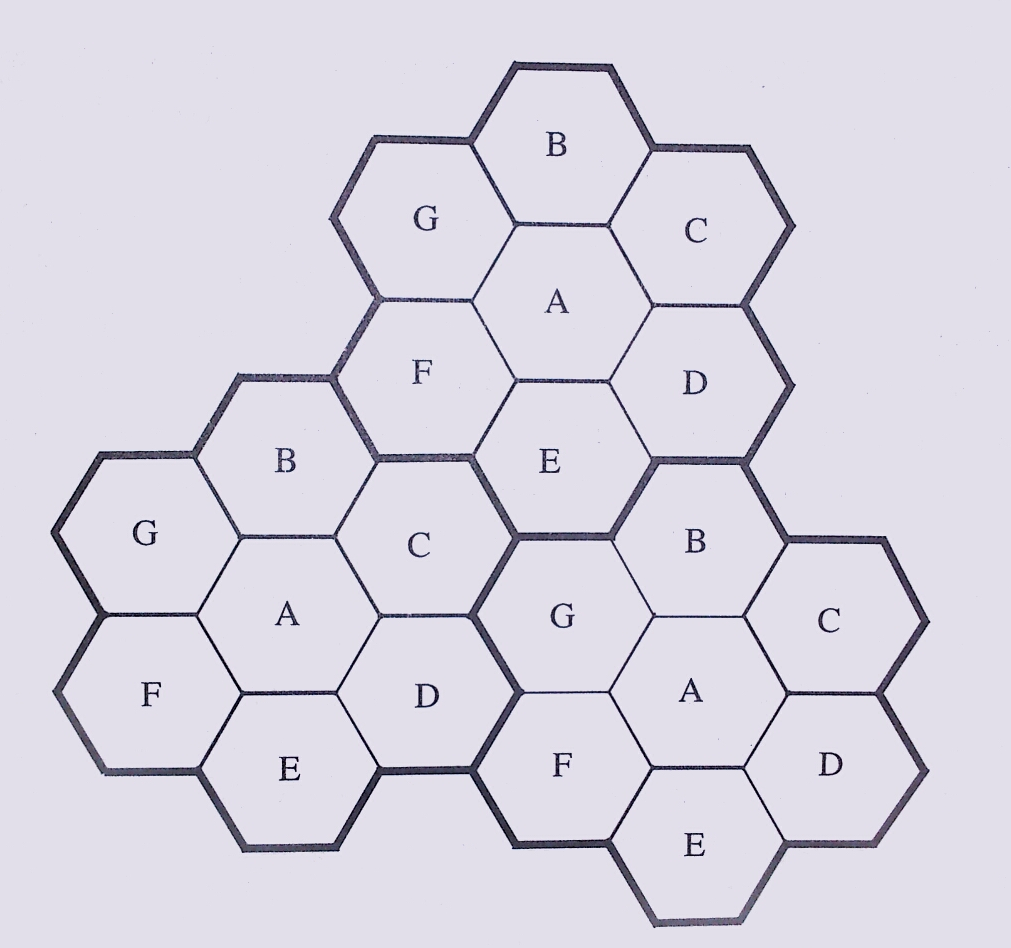
\includegraphics[width=\textwidth]{./01.introduction/img/frequency_reuse.png}
        \caption{Frequency reuse factor of $1 / 7$.}
        \label{fig:freuse}
    \end{subfigure}
    % Comment out the line break that is introduced with the blank line
    % so that it does not put the images one on top of the other...
    \begin{subfigure}[b]{0.45\textwidth}
        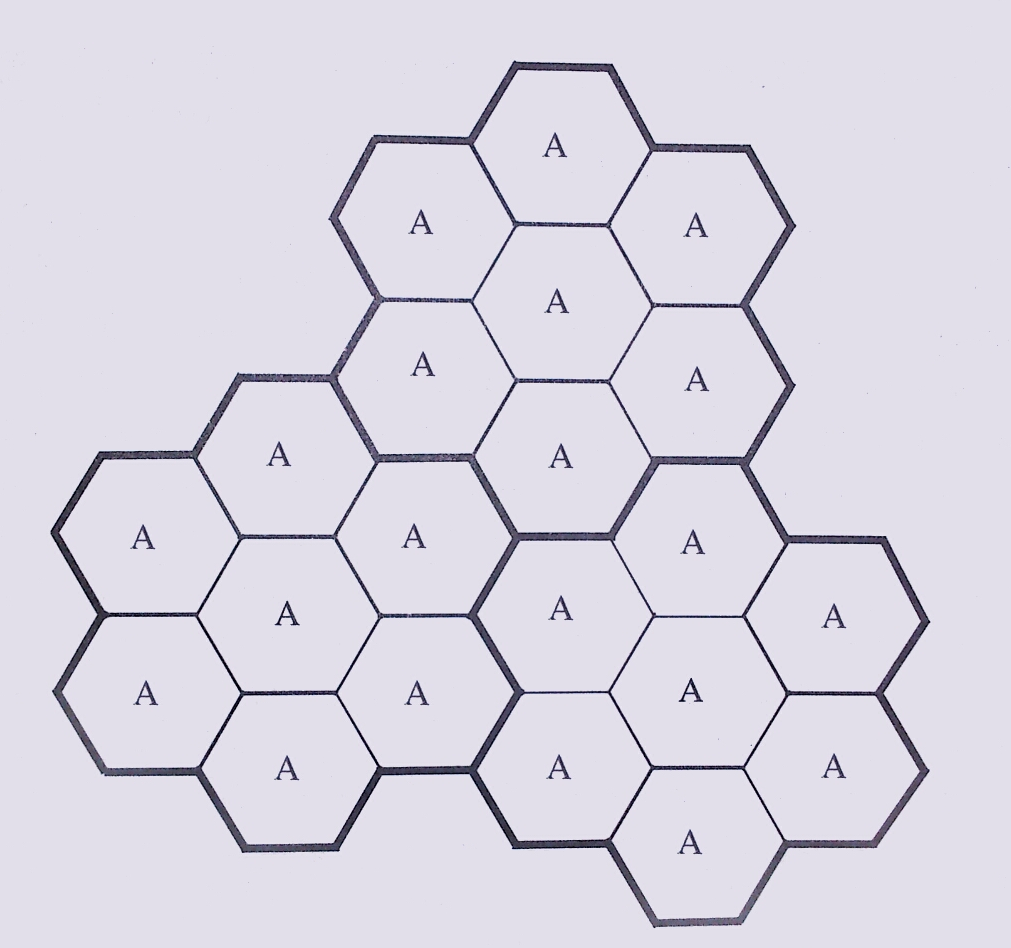
\includegraphics[width=\textwidth]{./01.introduction/img/universal_freq_reuse.png}
        \caption{Frequency reuse factor of $1$. {\color{red} DO NOT FORGET TO NOT EMPHASIZE THE 7-CELL CLUSTERS BUT EACH CELL INDIVIDUALLY}}
        \label{fig:ufreuse}
    \end{subfigure}
    \caption{Different frequency planning options}
    \label{fig:freq_plan}
\end{figure}

Current \gls{mimo} systems used in cellular networks are not achieving the
expected performance predicted by the initial theoretical works. The main reason
for this is the interference that is present naturally in cellular systems when
all cells share the same spectrum for the tranmissions. The effect of this
interference is a reduction of the \gls{sinr} experienced by the users, highly
reducing the advantages that \gls{mimo} could potentially deliver.

The conventional approach for cellular networks was to perform a careful
frequency planning in order to avoid the interference among neighboring cells.
Clusters of $N$ cells were grouped together, and assigned $N$ frequency bands to
be used, and the pattern is repeated for different clusters, yielding what is
called a \emph{frequency reuse factor} of $1/N$, as exemplified in
\reff{fig:freuse}.

The problem that this poses is that the available spectrum must be split, which
is an inherent inefficiency in the use of the resources.

A different option consists on a system where all the cells share a common
spectrum, so that all of them can use the full amount of resources available.
This is called \gls{ufr}, and a graphical description can be seen in
\reff{fig:ufreuse}.

It is in this kind of networks that the need for coordination among cells
arises, as every cell will interfere with the rest of the cells in the system
reducing the \gls{sinr} operating point of the users.

In the search for higher data rates and a more efficient use of the resources,
\gls{ufr} is a must to make the most out of the scarce resource that the radio
frequency spectrum is. Therefore, ``A new look at the interference''
\cite{gesbert10} is needed. The conventional concept of the interference as
being an impairment needs to shift to a new point of view where the interference
can be used to improve the overall performance of the network. A joint
optimization of the resources among all the cells is required in order to
globally improve the perfomance of the system \cite{gesbert07}.

The \gls{comp} operation considered in \cite{3gpprel11} is just a part of a much
broader field of multicell cooperation or coordinated communications where
several cells are assumed to cooperate, in the sense that they take measures in
order to alleviate to a certain degree the level of interference introduced into
other parts of the network, or the use of that interference to their advantage.

Intuitively, the best strategy should be to allow all the \glspl{bs} in the
network to cooperate, what is known as \emph{global coordination}. Even though
it may seem that global coordination may solve all the problems of frequency
planning and resource allocation, it cannot be ignored that it comes at a
non-negligible cost. The \glspl{bs} in the network may need to interchange
information in order to cooperatively transmit the information to all the users
in the system. The amount of information that needs to be exchanged grows out of
control with the size of the network, \ie the number of \glspl{bs} that form the
system. The result of this is that the capacity required to transmit this
information renders the alleged solution useless. Not only are the backhaul
transmission capabilities required prohibitive, but also tight synchronization
among the \glspl{bs} becomes a challenge, and channel information gathering
becomes a cumbersome task. Apart from this, theoretical works \cite{lozano13}
have unveiled intrinsic limitations of cooperation, whose benefits do not
unboundedly grow with the size of the coordination group.

For all these reasons, clustering appears as a means to cope with the
limitations of global coordination. In clustering, the coordination is not
performed among all the \glspl{bs} in the network but, instead, small groups, or
clusters, are formed and the cooperation takes place locally within the cluster.
This greatly reduces the amount of control information that should be handled by
the backhaul. Also, the reduced size of the group makes the system work at an
operating point where the natural limitations mentioned in \cite{lozano13} do
not affect the performance of the network.

\begin{figure}[t]
    \centering
    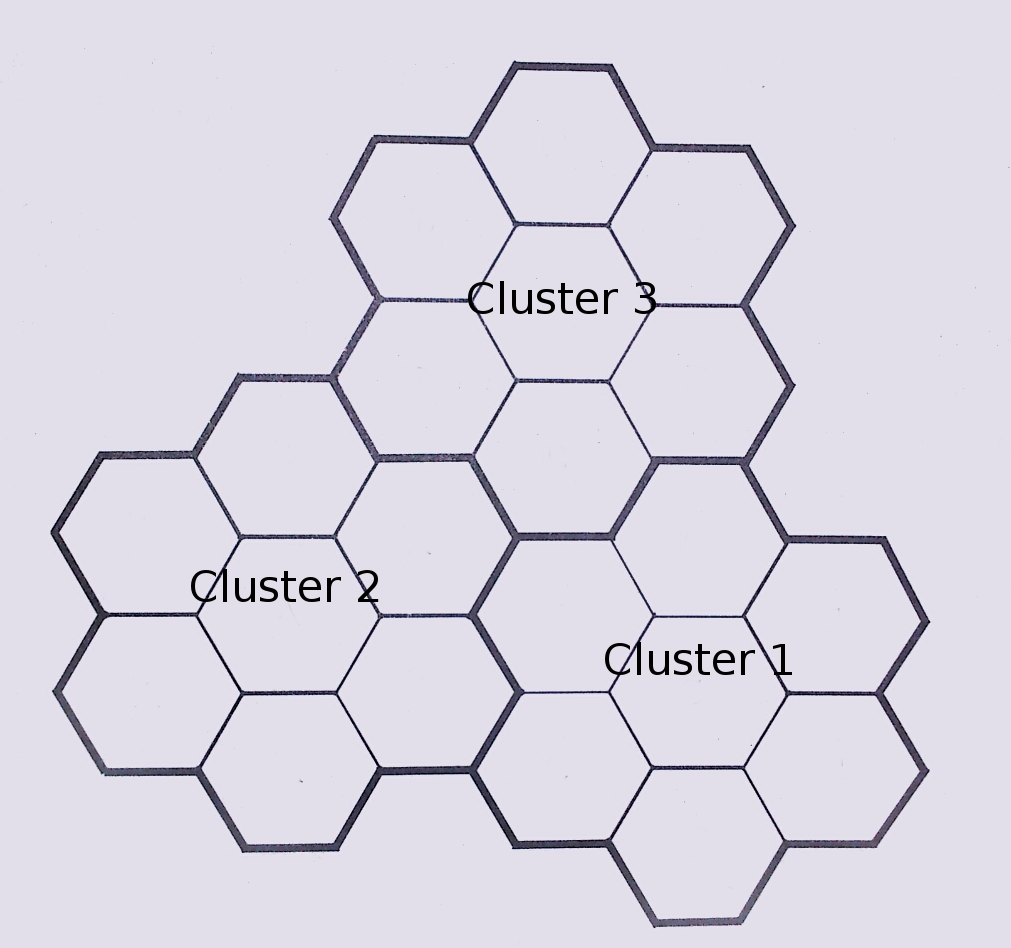
\includegraphics[width=0.45\textwidth]{./01.introduction/img/clustered_network.png}
    \caption{Clustered network scenario.}
    \label{fig:clustered_network}
\end{figure}

A schematic representation of a clustered network can be seen in
\reff{fig:clustered_network} where three clusters of seven cells are shown.

Grouping the cells in reduced size clusters has an important drawback: If the
cooperation is done within a cluster and neighboring clusters are not
coordinated in any way, there would be, again, unhandled interference, albeit
not the same as in the uncoordinated scenario.

This thesis focuses on a clustered cellular network where \gls{bd} is used for
coordination within each cluster. The performance of the network, in terms of
achievable rate and fairness considerations, is analyzed and its dependence on
several parameters of the network is studied. Also, mechanisms to deal with the
interference, resulting from clustering, are presented.

The main contributions of this thesis are:

\begin{itemize}
    \item \fullcite{corvaja13b}
    \item \fullcite{corvaja14}
    \item \fullcite{jjgarcia14}
\end{itemize}

The organization of the present document is as follows:

\begin{itemize}
    \item In \refc{ch:state_art} a compilation of different alternatives for
        coordination, as well as for clustering, found in the literature are
        presented and described.
    \item \refc{ch:system_model} presents the system model used throughout the
        dissertation, and describes in detail \gls{bd} and the power allocation
        strategies used in the rest of the work.
    \item \refc{ch:achiev_rates} analyzes the performance of a cellular network,
        in terms of the mean achievable rate as a function of the cluster size,
        when using \gls{bd} for coordination within each cluster, and taking
        into account the interference due to external clusters. An analytical
        expression for the mean achievable rate is developed and the optimum
        cluster size is obtained.
    \item \refc{ch:rate_statistics} considers the fairness of the system, and
        studies the variability of the rate, as a complement to the mean
        obtained in \refc{ch:achiev_rates}. The behavior of the rates is shown
        to follow almost exactly a Gamma distribution.
    \item The pernicious effect of the \gls{oci} in the rates is introduced in
        \refc{ch:adaptive_schedule}, and a mechanism to deal with it, based on
        a mixed tranmission strategy and on a scheduling algorithm, is
        presented.
    \item Finally, some conclusions and future research lines are discussed in
        \refc{ch:conclusions_and_future}.
\end{itemize}


% State of the art
\chapter{Block Diagonalization}\label{ch:bd}


% System Model
\chapter{System Model}\label{ch:system_model}

% ------------------------------------------------------------------------------
\section{System Model}\label{sec:system_model}
The system that will be considered throughout this work aims to represent the
downlink of a canonical cellular network, comprising several identical cells,
layed out over a regular hexagonal grid.

When studying a cellular network, the cells located at the edge of the network
will not experience the same conditions as the cells in the center of the
network. A typical way to deal with this situation is to consider a scenario
that wraps around (\reff{fig:torus_scenario}) so that cells on one side of the
scenario affect cells on the opposite side. Another option is to consider a
scenario with more cells than necessary, and then analyze the behavior of the
cells located within the center of the network (\reff{fig:interfering_scenario})
, so that the exterior cells account for the interference, equaling the
conditions of all the cells in the network.

\begin{figure}[t]
   \centering
   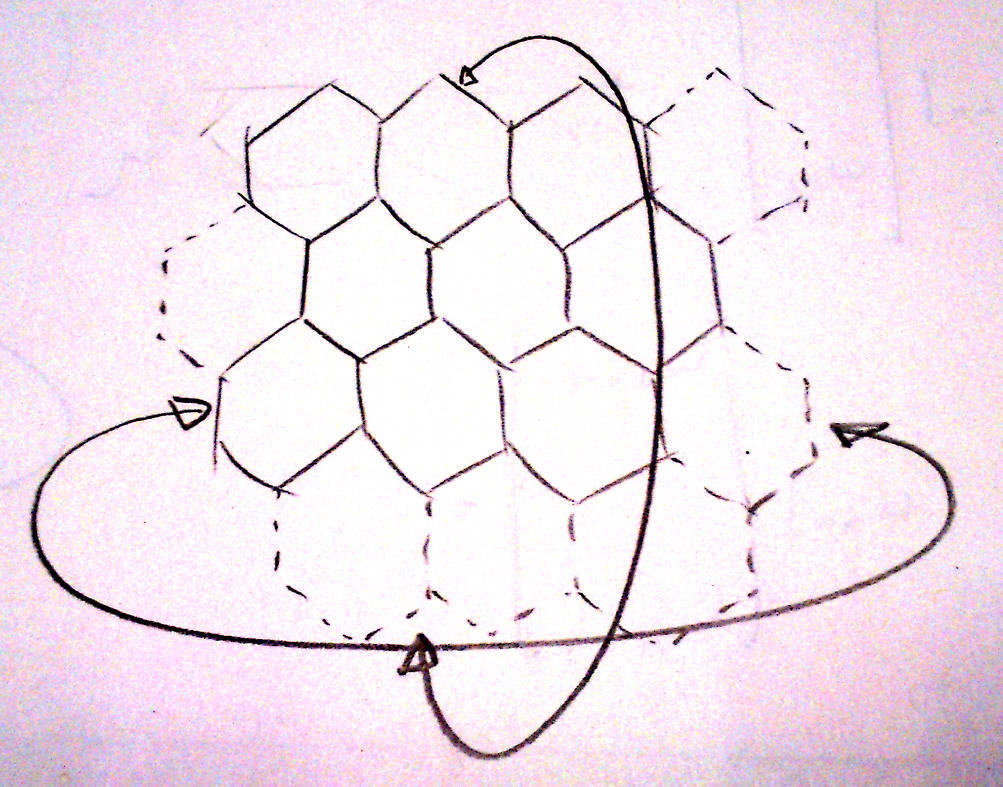
\includegraphics[width=0.5\textwidth]{./03.system_model/img/torus_scenario}
   \caption{Wrap around scenario. Cells on one side of the scenario influence
            the cells on the other side as if they were next to each other.}
   \label{fig:torus_scenario}
\end{figure}

\begin{figure}[t]
   \centering
   \includegraphics[width=0.5\textwidth]{./03.system_model/img/interfering_scenario}
   \caption{Oversized scenario. The behavior of the network is analyzed in the
            central cells of the network, and the exterior cells compensate the 
            network edge effects.}
   \label{fig:interfering_scenario}
\end{figure}

Each cell in the system under study will be served with a single \gls{bs} that
is equipped with $t$ transmit antennas. Each of the users considered in the
system has $r$ receive antennas.

A system with $M$ \gls{bs} and $N$ users can then be modelled as

\begin{equation} \label{eq:generic_system_model}
    \yy = \HH \xx + \nn
\end{equation}

$\yy$ represents the signal received at all the users and is defined as

\begin{equation} \label{eq:generic_rx_signal}
    \yy = \begin{bmatrix}
            \yy_1\\
            \vdots\\
            \yy_N
        \end{bmatrix} \in \C^{Nr \times 1}
\end{equation}

\noindent
where $\yy_i \in \C^{r \times 1}$ is the signal received at the $i$-th user.

$\HH$ is the channel matrix from all the \gls{bs} to all the users, with the
following structure

\begin{equation} \label{eq:generic_ch_mat}
    \HH = \begin{bmatrix}
            \HH_{11} & \cdots & \HH_{1M}\\
            \vdots   & \ddots & \vdots\\
            \HH_{N1}  & \cdots & \HH_{NM}
    \end{bmatrix} \in \C^{Nr \times Mt}
\end{equation}

\noindent
where $\HH_{ij} \in \C^{r \times t}$ represents the channel matrix from the
$j$-th \gls{bs} to the $i$-th user. It will include the path loss due to
propagation, small scale fading, shadowing, and any other characteristic of
the radio channel that needs to be taken into consideration.

$\xx$ is the signal transmitted from all the \gls{bs}, and it is composed of

\begin{equation} \label{eq:generic_tx_signal}
    \xx = \begin{bmatrix}
        \xx_1 \\
        \vdots \\
        \xx_M
    \end{bmatrix} \in \C^{Mt \times 1}
\end{equation}

\noindent
where $\xx_j \in \C^{t \times 1}$ is the signal transmitted by the $j$-th
\gls{bs}. Additionally, the power transmitted by the $j$-th \gls{bs} can be
calculated from the transmitted signal as

\begin{equation} \label{eq:bs_tx_power}
P_{j,\tx} = \Tr \left(\xx_j \xx_j^H\right) = \xx_j^H \xx_j
\end{equation}

\noindent
and each \gls{bs} will have an independent power constraint

\begin{equation} \label{eq:pbpc}
    P_{j,\tx} \leq P_{j, \max}
\end{equation}

Finally $\nn$ represents the \gls{awgn} at all the receivers

\begin{equation} \label{eq:generic_noise}
    \nn = \begin{bmatrix}
        \nn_1 \\
        \vdots \\
        \nn_N
    \end{bmatrix} \in \C^{Nr \times 1}
\end{equation}

\noindent
with $\nn_i \in \C^{r \times 1}$ accounts for the Gaussian noise at the $i$-th
receiver. Throughout this work $\nn_i$ is considered to be formed by \emph{iid}
entries, drawn from a zero mean, $\sigma_i^2$ variance Gaussian distribution,
$\nn_i \sim \mathcal{N}\left(\zero, \sigma_i^2 \eye\right)$. The noise variance
will be assumed the same for all the receivers.

In a general scenario, there may be cooperation among the \gls{bs} in the system
so that the information intended for a particular user will be transmitted by
several or all the \gls{bs}. Or, equivalently, each \gls{bs} transmits a
combination of the information of several users

\begin{equation} \label{eq:generic_tx_precod}
    \xx_j = \Wtx_{j1} \ss_1 + \cdots + \Wtx_{jN} \ss_N
\end{equation}

\noindent
where $\ss_i \in \C^{\ell \times 1}$ is the vector of information symbols to be
transmitted to user $i$, with $\ell$ being the number of simultaneous symbols or
streams to be transmitted to that user. $\Wtx_{ji} \in \C^{t \times \ell}$ is
the precoding matrix used at the $j$-th transmitter for the data of the
$i$-th user.

It will be assumed that the information symbols are independent and drawn from a
Gaussian distribution such that $\ss_i \sim \mathcal{N}\left(\zero, \RR_{\ss_i}
\right)$, where $\RR_{\ss_i} = \diag\left\{p_{i1}, \ldots, p_{i\ell}\right\} \in
\R^{\ell \times \ell}$ contains the power allocated to each of the symbols in
$\ss_i$. The transmitted power can be expressed as

\begin{equation} \label{eq:bs_precod_power}
    P_{j, \tx} = \sum\limits_{i=1}^{N} \Tr \left( \Wtx_{ji} \RR_{\ss_i}
    \WtxH_{ji} \right)
\end{equation}

The choice of the precoding matrices and of the receiving filter will determine
the transmission strategy used. This Thesis will focus mainly on \gls{bd}
\cite{spencer04} which is described in \refs{sec:bd}.

On the receiver side, no cooperation among the users will be considered, so each
user may perform, independently, additional processing of the received signal by
applying a linear filter or equalizer

\begin{equation} \label{eq:generic_rx_eq}
    \hat{\ss}_i = \Wrx_i \yy_i
\end{equation}

\noindent
where $\Wrx_i \in \C^{r \times \ell}$ is the equalizer used at the $i$-th
receiver.

Combining \eqref{eq:generic_system_model}--\eqref{eq:generic_tx_precod} it is
possible to rewrite \eqref{eq:generic_system_model} as

\begin{equation} \label{eq:system_model}
    \yy = \HH \Wtx \ss + \nn
\end{equation}

\noindent
where

\begin{equation} \label{data_symbols}
    \ss = \begin{bmatrix}
        \ss_1 \\
        \vdots \\
        \ss_N
    \end{bmatrix} \in \C^{N\ell \times 1}
\end{equation}

\noindent
and the global precoding matrix is

\begin{equation} \label{eq:precoding_matrix}
    \Wtx = \begin{bmatrix}
        \Wtx_{11} & \cdots & \Wtx_{1N} \\
        \vdots    & \ddots & \vdots \\
        \Wtx_{M1} & \cdots & \Wtx_{MN} \\
    \end{bmatrix} \in \C^{Mt \times N\ell}
\end{equation}

\noindent
and it can be partitioned as

\begin{equation} \label{eq:precod_partition}
    \Wtx = \left[ \Wtx_1, \ldots, \Wtx_N \right]
\end{equation}

\noindent
with

\begin{equation} \label{eq_precod_user}
    \Wtx_i = \begin{bmatrix}
        \Wtx_{11} \\
        \vdots \\
        \Wtx_{M1}
    \end{bmatrix} \in \C^{Mt \times \ell}
\end{equation}

The channel matrix can then be partitioned as

\begin{equation} \label{eq:ch_mat_partition}
    \HH = \begin{bmatrix}
        \HH_1 \\
        \vdots \\
        \HH_N
    \end{bmatrix}
\end{equation}

\noindent
where $\HH_i \in \C^{r \times Mt}$ is the channel matrix from all the \gls{bs}
to the $i$-th user.

As it has already been mentioned, receiver cooperation is not going to be
considered, so looking at a particular user, \emph{e.g.} the $i$-th user, the
signal that is received will be

\begin{equation} \label{eq:rx_signal_user}
    \yy_i = \HH_i \Wtx \ss + \nn_i
\end{equation}

\noindent
which can be rewritten as

\begin{equation} \label{eq:rx_signal_user_interf}
    \yy_i = \HH_i \Wtx_i \ss_i +
    \underbrace{\sum\limits_{\substack{j = 1\\j \neq i}}^{N} \HH_i
        \Wtx_j \ss_j}_{\text{Interference}} + \nn_i
\end{equation}

\noindent
so that it can be readily seen how other users' data appear as an interference
term that degrades the received signal.

Defining the term of interference plus noise as

\begin{equation} \label{eq:interf_plus_noise}
    \zz_i = \sum\limits_{\substack{j = 1\\j \neq i}}^{N} \HH_i \Wtx_j
    \ss_j + \nn_i
\end{equation}

and using \eqref{eq:rx_signal_user_interf}, the ergodic (mean) rate for the
$i$-th user is given by \cite{cover_thomas}, \cite{holter01}

\begin{equation} \label{eq:generic_ergodic_capacity}
    R_i = \mathbb{E}\left\{
        \log_2\left| \eye + \HH_i\Wtx_i\RR_{\ss_i}\WtxH_i\HH_i^H \RR_{\zz_i}^{-1}
    \right|
    \right\}
\end{equation}

\noindent
where $\RR_{\zz_i} \in \C^{r \times r}$ is the covariance matrix of the noise plus
the interference term in \eqref{eq:rx_signal_user_interf}

\begin{equation} \label{eq:r_in}
    \RR_{\zz_i} = \zz_i \zz_i^H = 
    \left(\sum\limits_{\substack{j=1\\j\neq i}}^{N} \HH_i\Wtx_j+\nn_i
    \right)
    \left(\sum\limits_{\substack{j=1\\j\neq i}}^{N} \HH_i\Wtx_j+\nn_i
    \right)^H
\end{equation}

In the rest of the work, there are a set of assumptions that will be made,
mainly to guarantee the feasibility of some of the results obtained:

\begin{itemize}
    \item The number of users will be the same as the number of \gls{bs},
        \emph{i.e.} $N = M$.
    \item The total number of antennas transmitting will be greater or equal
        than the total number of antennas at the receiver side, this is $Mt
		\geq Nr$.
    \item The number of streams transmitted to each user must be $\ell \leq r$.
    \item There is no correlation, neither at the transmitters nor at the
        receivers, so that $\HH$ is full rank or, equivalently, $\rank\left(
        \HH\right) = \min\left(Nr,Mt\right)$. As $Mt \geq Nr$, then $\rank\left(
        \HH\right) = Nr$.
\end{itemize}

% ------------------------------------------------------------------------------
\section{Block Diagonalization}\label{sec:bd}

One possibility to cancel the inter-user interference is to diagonalize the
channel matrix. Perfect diagonalization is only possible if $Mt \geq Nr$
\cite{caire03}, and it is achieved using the following precoding matrix

\begin{equation} \label{eq:zf_precod}
    \Wtx = \HH^\dagger
\end{equation}

This solution is optimum only when every user has only one antenna. In the case
under study, with multiantenna receivers, complete diagonalization of the
channel matrix is suboptimal since each user is able to coordinate the
processing of its received signal.

In \cite{spencer04} is stated that the optimum solution under the constraint
that all inter-user interference be zero is obtained with $\HH \Wtx$ being
block diagonal. In \cite{spencer04}, \gls{bd} is proposed as an algorithm to
obtain a precoding matrix that is able to block diagonalize the channel matrix.
This algorithm is described next.

In order to meet the condition of zero inter-user interference, it is necessary
to cancel the interference term in \eqref{eq:rx_signal_user_interf}, and this
is equivalent to meet the following

\begin{equation} \label{eq:cancel_interf}
    \HH_i \Wtx_j = \zero \text{\quad } \forall j \neq i
\end{equation}

Let $\Htilde_i$ be the channel matrix $\HH$ without $\HH_i$, \emph{i.e.}

\begin{equation} \label{eq:h_tilde}
    \Htilde_i = \begin{bmatrix}
        \HH_1 \\
        \vdots \\
        \HH_{i - 1} \\
        \HH_{i + 1} \\
        \vdots \\
        \HH_N
    \end{bmatrix} \in \C^{(N - 1)r \times Mt}
\end{equation}

Then the condition \eqref{eq:cancel_interf} can be obtained making $\Wtx_i$ lie
in the null space or kernel of $\Htilde_i$. This is possible only if the
dimension of the null space is greater than zero, \emph{i.e.} $\rank\left(\ker
\left(\Htilde_i\right)\right) > 0$.

Now, with the dimensions of $\Htilde$, the rank of its null space is

\begin{equation} \label{eq:rank_kern_htilde}
   \rank\left(\ker\left(\Htilde_i\right)\right) = Mt - \rank\left(\Htilde_i
   \right)
\end{equation}

But it is assumed that $\HH$ is full rank, ergo $\rank\left(\Htilde_i\right) =
(N - 1)r = \Ltilde_i$, and then

\begin{equation} \label{eq:rank_kern_htilde_ok}
    \rank\left(\ker\left(\Htilde_i\right)\right) = Mt - \Ltilde_i > 0
\end{equation}

\noindent
so it is guaranteed that a precoding matrix $\Wtx_i$ that lies in the null space
of $\Htilde_i$ exists.

The simplest way to obtain such $\Wtx_i$ involves using the \gls{svd} of the
matrix $\Htilde_i$.

Let $\Htilde_i$ be decomposed as

\begin{equation} \label{eq:htilde_svd}
    \Htilde_i = \Utilde_i \bLambdatilde_i \left[ \Vtilde_i^{(1)}, \Vtilde_i^{(0)}
    \right]^H
\end{equation}

\noindent
where $\Vtilde_i^{(0)} \in \C^{Mt \times (Mt - \Ltilde_i)}$ contains the last
$Mt - \Ltilde_i$ right singular vectors of $\Htilde_i$, corresponding to the
singular values equal to zero. $\Vtilde_i^{(0)}$ forms an orthonormal basis of
the null space of $\Htilde_i$, and thus its columns can be used to cancel the
inter-user interference

\begin{equation} \label{eq:v0_zero_interf}
    \Htilde_i \Vtilde_i^{(0)} = \zero
\end{equation}

Using these matrices as precoding the result is

\begin{equation} \label{eq:block_diag}
    \Hhat = \HH \begin{bmatrix}
        \Vtilde_1^{(0)}, \ldots, \Vtilde_N^{(0)}
    \end{bmatrix} = \begin{bmatrix}
        \HH_1 \Vtilde_1^{(0)} &        & \zero \\
                              & \ddots & \\
        \zero                 &        & \HH_N \Vtilde_N^{(0)}
    \end{bmatrix}
\end{equation}

\noindent
that, as it can be seen, has a block diagonal structure, which gives the name to
the algorithm proposed in \cite{spencer04}.

The next problem that \gls{bd} solves is the maximization of the sum rate of the
system, given the block diagonal structure in \eqref{eq:block_diag}. The
precoding matrix $\Wtx_i$ will be considered to be

\begin{equation} \label{eq:wtx_nosvd}
    \Wtx_i = \Vtilde_i^{(0)} \WW_i^{\prime}
\end{equation}

\noindent
where $\WW_i^{\prime} \in \C^{(Mt - \Ltilde_i) \times \ell}$ will take care of
the rate maximization.

Introducing \eqref{eq:wtx_nosvd} into \eqref{eq:generic_ergodic_capacity} the
ergodic capacity simplifies to

\begin{equation} \label{eq:bd_ergodic_capacity_nosvd}
    R_i^{\text{no interf}} = \mathbb{E}\left\{
        \log_2\left| \eye + \frac{1}{\sigma_i^2}\Hhat_i\WW_i^{\prime}
        \RR_{\ss_i} \WW_i^{\prime,H}\Hhat_i^H
    \right|
    \right\}
\end{equation}

\noindent
where $\Hhat_i = \HH_i\Vtilde_i^{(0)} \in \C^{r \times (Mt - \Ltilde_i)}$.

In order to maximize the rate, consider the \gls{svd}

\begin{equation} \label{eq:svd_max_rate}
    \Hhat_i = \Uhat_i \begin{bmatrix}
        \bLambdahat_i & \zero \\
        \zero        & \zero
    \end{bmatrix} \left[ \Vhat_i^{(1)}, \Vhat_i^{(0)} \right]^H
\end{equation}

\noindent
where $\bLambdahat_i = \diag\left\{\lambdahatsqrt_{i1}, \ldots,
\lambdahatsqrt_{ir} \right\} \in \C^{r \times r}$ contains the non zero singular
values of $\Hhat_i$ , which has $\rank\left(\Hhat_i\right) = r$. And
$\Vhat_i^{(1)} \in \C^{(Mt - \Ltilde_i) \times r}$ contains the first $r$ right
singular vectors of $\Hhat_i$ , and it will be used as $\WW_i^{\prime}$,
yielding the following precoding matrix

\begin{equation} \label{eq:bd_precod}
    \Wtx_i = \Vtilde_i^{(0)} \Vhat_i^{(1)}
\end{equation}

The \gls{bd} also provides the receiver filter to be used at each user which
will be

\begin{equation} \label{eq:bd_eq}
    \Wrx_i = \Uhat_i^H
\end{equation}

Using all of the above, the rate that the $i$-th user can obtain is given by the
expression

\begin{equation} \label{eq:bd_ergodic_capacity}
    R_i^{\text{BD}} = \mathbb{E}\left\{
        \sum\limits_{k = 1}^{\ell} \log_2 \left(1 + \frac{\lambdahat_{ik}
        p_{ik}}{\sigma_i^2} \right)
    \right\}
\end{equation}

\noindent
where the only parameters left to be computed are the power allocated to each of
the $\ell$ streams of each user, and different options to do it will be
discussed in \refs{sec:power_allocation}.

% ------------------------------------------------------------------------------
\section{Power Allocation}\label{sec:power_allocation}

In \refs{sec:bd}, the \gls{bd} algorithm has been described to get the precoding
matrix to be used at the transmitter and the equalization filter to be used at
the receiver side. After \gls{bd} has been used, the power should be allocated
to each of the data streams of each user, this is, the $p_{ij}$ in
\eqref{eq:bd_ergodic_capacity} should be calculated in order to achieve a given
performance, and subject to particular constraints.

The need for a power allocation algorithm comes from the restriction on the
maximum power available for transmission, which may be due to physical
limitations, or regulatory issues.

There are several different power constraints:

\begin{itemize}
    \item \gls{papc}: The maximum power is constrained for each antenna at the
        transmitter. This option is specially well suited for distributed
        antenna systems \cite{choi07}, \cite{lee12}.
    \item \gls{pbpc}: In this case the maximum power is limited per base station
        instead of per antenna. This option is more appropriate for scenarios
        where all the transmitting antennas are collocated and may share a power
        budget, so that the transmission power can be arbitrarily allocated to
        each of the transmitter antennas.
\end{itemize}

A \gls{tpc} can also be considered, which assumes that the maximum power is
shared among all the transmitters in the system. Although this system is more
easily analyzed, it is very unrealistic so it will not be considered in this
work, except in \refss{ssec:scaled_wf} where a \gls{tpc} is used to obtain an
intermediate result.

For the sake of simplicity, \gls{pbpc} will be used for the different analyses. In any case, \gls{papc} can be seen as a particularization of \gls{pbpc} as the
derivations shown in this section can be applied to a \gls{papc} system
considering instead of each \gls{bs} to have $t$ transmit antennas, $t$ single
antenna \gls{bs}.

The problem that needs to be solved is, in general, the maximization of some
function of the rate of each of the users subject to a \gls{pbpc}

\begin{equation} \label{eq:generic_optim_problem}
\begin{aligned}
	&\maxi\limits_{\left\{\RR_{\ss_i}\right\}} &&\quad f\left(R_i^{\text{BD}}
    \left(\RR_{\ss_1},\right), \ldots, R_N^{\text{BD}}\left(\RR_{\ss_N}\right)
    \right) \\
	&\st &&\quad P_{j, \tx} \leq P_{j, \max},\quad j = 1, \ldots, M
\end{aligned}
\end{equation}

One common metric used for the maximization is the weighted sum-rate of the
system, so that the function $f\left(\cdot\right)$ is equal to

\begin{equation} \label{eq:weighted_sum_rate}
    f\left(R_i^{\text{BD}}, \ldots, R_N^{\text{BD}}\right) =
    \sum\limits_{i = 1}^{N}\alpha_i R_i^{\text{BD}}
\end{equation}

\noindent
where $\alpha_i \in \left[0, 1\right]$ can be seen as different priorities for
different users, and they are assumed to be

\begin{equation} \label{eq:priorities}
    \sum\limits_{i = 1}^{N}\alpha_i = 1
\end{equation}

\noindent
and in the particular case where all the $\alpha_i = 1/N$, then the function
$f\left(\cdot\right)$ represents the sum-rate of the system.

Calling

\begin{equation} \label{eq:precoding_bs}
	\WtxBar_j = \left[\Wtx_{j1}, \ldots, \Wtx_{jN}\right] \in \C^{t \times
	N\ell}
\end{equation}

\noindent
the precoding matrix of the $j$-th \gls{bs}, and

\begin{equation} \label{eq:powers_all_users}
	\RR_{\ss} = \blkdiag \left(\RR_{\ss_1}, \ldots, \RR_{\ss_N}\right) \in
	\C^{N\ell \times N\ell}
\end{equation}

\noindent
the matrix containing the power assigned to all the streams of all the users,
the power constraint in \eqref{eq:generic_optim_problem} can then be
reformulated as

\begin{equation} \label{eq:pbpc_constraint}
	\Tr \left( \WtxBar_j\RR_{\ss}\WtxHbar_j \right) \leq P_{j,\max}
\end{equation}

Now the term inside the trace operator can be written explicitly as a function
of $p_{ik}$ in order to make it easier to analyze. First define

\begin{equation} \label{eq:precoding_bs_columns}
	\WtxBar_j = \left[ \wbar_{j,11}, \ldots, \wbar_{j, 1\ell}, \ldots,
	\wbar_{j,N\ell} \right]
\end{equation}

\noindent
where $\wbar_{j, ik} \in \C^{t \times 1}$ is the $ik$-th column of $\WtxBar_j$,
\emph{i.e.} the precoding that is used at the $j$-th \gls{bs} for the $k$-th
stream of the $i$-th user.
And then:

\begin{equation}
\begin{aligned}
	\WtxBar_j\RR_{\ss}\WtxHbar_j = &\left[\wbar_{j,11}, \ldots, \wbar_{j, N\ell}
	\right]
	\begin{bmatrix}
		p_{11} &        & 0\\
               & \ddots &  \\
		0      &        & p_{N\ell}

	\end{bmatrix}
	\begin{bmatrix}
		\wbar_{j,11}^H\\
		\vdots\\
		\wbar_{j,N\ell}^H
	\end{bmatrix} = \\
	= & p_{11}\wbar_{j,11}\wbar_{j,11}^H + \cdots + p_{N\ell}\wbar_{j,N\ell}
	\wbar_{j,N\ell}^H \\
	= & \sum\limits_{i = 1}^N\sum\limits_{k = 1}^\ell p_{ik}
	\wbar_{j,ik}\wbar_{j,ik}^H
\end{aligned}
\end{equation}

\noindent
and the trace is

\begin{equation} \label{eq:trace_terms_p_i}
	\Tr\left(\WtxBar_j \RR_{\ss} \WtxHbar_j\right) = \sum\limits_{i = 1}^N
	\sum\limits_{k = 1}^\ell p_{ik} \left\| \wbar_{j, ik} \right\|_2^2
\end{equation}

\noindent
where

\begin{equation} \label{eq:norm2}
    \left\|\wbar_{j,ik}\right\|_2^2 = \Tr\left( \wbar_{j,ik} \wbar_{j,ik}^H
    \right) = \wbar_{j,ik}^H \wbar_{j,ik}.
\end{equation}

The sum-rate maximization problem can then be formulated in \emph{standard form}
\cite{boyd_convex} as

\begin{equation} \label{eq:sum_rate_maxim}
\begin{aligned}
	&\mini\limits_{p_{ik}} &&-\sum\limits_{i = 1}^N
	\sum\limits_{k = 1}^\ell \log_2\left( 1 +
	\frac{\lambdahat_{ik} p_{ik}}{\sigma_i^2} \right)\\
	&\st &&\sum\limits_{i = 1}^N \sum\limits_{k = 1}^\ell p_{ik} \left\|
	\wbar_{j,ik} \right\|_2^2 - P_{j,\max} \leq 0, &&
    \begin{array}{l}
        j = 1, \ldots, M
    \end{array}\\
    & &&-p_{ik} \leq 0, &&
	\begin{array}{l}
	i = 1, \ldots, N\\
	k = 1, \ldots, \ell
	\end{array}
\end{aligned}
\end{equation}

In the next sections, different alternatives for obtaining these powers are
presented and described.

% ------------------------------------------------------------------------------
\subsection{Optimal Power Allocation}\label{ssec:optimal_power_allocation}

In \eqref{eq:sum_rate_maxim}, the function $\log_2(\cdot)$ is convex on $p_{ik}$
 and the sum of convex functions is also convex, so the objective function in
\eqref{eq:sum_rate_maxim} is convex. The constraints are affine and therefore
convex too. The optimization problem in \eqref{eq:sum_rate_maxim} is a convex
optimization problem that can be solved using a myriad of numerical technics
\cite{boyd_convex}. Nonetheless, it would be interesting to analyze a bit
further the problem in order to get some insight about it.

The problem in \eqref{eq:sum_rate_maxim} satisfies \emph{Slater's condition}
\cite{boyd_convex} since the objective function is convex and all the
inequality constraints are affine, hence \emph{strong duality} holds. This means
that the optimum value of the primal problem is equal to the optimum value of
the \emph{Lagrange dual problem}, so that this can be used to find out the
solution to the primal, original, problem.

Under these conditions, and considering that the objective function is
differentiable with respect to $p_{ik}$, \gls{kkt} conditions \cite{boyd_convex}
are necessary and sufficient for optimality of a solution, and they can be used
to analyze the optimization problem in search for an optimal solution. The
\gls{kkt} conditions for \eqref{eq:sum_rate_maxim} are

\begin{equation} \label{eq:kkt_conditions}
\begin{array}{rccl}
	\sum\limits_{i = 1}^N \sum\limits_{k = 1}^\ell p_{ik}^\ast \left\|
    \wbar_{j,ik} \right\|_2^2 - P_{j,\max} & \leq & 0, &
    \begin{array}{l}
        j = 1, \ldots, M
    \end{array}\\

    p_{ik}^\ast &\leq & 0, &
	\begin{array}{l}
	i = 1, \ldots, N\\
	k = 1, \ldots, \ell
	\end{array}\\

    \nu_j^\ast & \geq & 0, &
    \begin{array}{l}
        j = 1, \ldots, M
    \end{array}\\

    \mu_{ik}^\ast & \geq & 0, &
	\begin{array}{l}
	i = 1, \ldots, N\\
	k = 1, \ldots, \ell
	\end{array}\\

    \nu_j^\ast\left(\sum\limits_{i = 1}^N \sum\limits_{k = 1}^\ell p_{ik}
    \left\|\wbar_{j,ik} \right\|_2^2 - P_{j,\max} \right) & = & 0, &
    \begin{array}{l}
        j = 1, \ldots, M
    \end{array}\\

    -\mu_{ik}^\ast p_{ik}^\ast & = & 0, &
	\begin{array}{l}
	i = 1, \ldots, N\\
	k = 1, \ldots, \ell
	\end{array}\\

    \nablabf_{\pp} \mathcal{L}\left(\pp^\ast, \mathbf{\nu}^\ast,
        \mathbf{\mu}^\ast \right) & = & \zero

\end{array}
\end{equation}

\noindent
where the superscript $^\ast$ represents a feasible solution of the optimization
problem, $\nablabf_{\pp}$ is the gradient with respect to the powers $\pp = 
\left[p_{11}, \ldots, p_{N\ell}\right]^T$, $\mathbf{\nu} = \left[\nu_1, \ldots,
\nu_M\right]^T$ and $\mathbf{\mu} = \left[\mu_{11}, \ldots, \mu_{N\ell}
\right]^T$ are the Lagrange multipliers, and $\mathcal{L}$ represents the
\emph{Lagrangian} associated with the problem \eqref{eq:sum_rate_maxim}, and it
is defined as

\begin{equation} \label{eq:lagrangian}
\begin{aligned}
    \mathcal{L}\left(\pp, \mathbf{\nu}, \mathbf{\mu}\right) =
    & -\sum\limits_{i = 1}^N
        \sum\limits_{k = 1}^\ell \log_2\left( 1 +
        \frac{\lambdahat_{ik} p_{ik}}{\sigma_i^2} \right) + \\
    & \sum\limits_{j = 1}^M \nu_j\left(
        \sum\limits_{i = 1}^N \sum\limits_{k = 1}^\ell p_{ik} \left\|
        \wbar_{j,ik} \right\|_2^2 - P_{j,\max}\right) - \\
    & \sum\limits_{i = 1}^N \sum\limits_{k = 1}^\ell \mu_{ik} p_{ik}
\end{aligned}
\end{equation}

The gradient of a function $f(\xx)$ with respect to $\xx \in \C^{n \times 1}$ is
defined as

\begin{equation} \label{eq:gradient}
    \nablabf_{\xx}f(\xx) = \begin{bmatrix}
        \frac{\partial}{\partial x_1}f(\xx) \\
        \vdots \\
        \frac{\partial}{\partial x_n}f(\xx)
    \end{bmatrix}
\end{equation}

First the gradient of the objective function is calculated, by computing the
partial derivatives

\begin{equation} \label{eq:gradient_objective}
    \frac{\partial}{\partial p_{ik}} \left\{
        -\sum\limits_{i = 1}^N
        \sum\limits_{k = 1}^\ell \log_2\left( 1 +
        \frac{\lambdahat_{ik} p_{ik}}{\sigma_i^2} \right)
    \right\} = \frac{-\lambdahat_{ik}}{\ln\left(2\right)\left(\sigma_i^2 +
    \lambdahat_{ik} p_{ik}\right)}
\end{equation}

And the same for the inequality constraints

% The comment in the middle of the `aligned` environment is intended so that it
% does not fail compiling
\begin{equation} \label{eq:gradient_constraints}
\begin{aligned}
    &\frac{\partial}{\partial p_{ik}} \left\{
    \sum\limits_{i = 1}^N \sum\limits_{k = 1}^\ell p_{ik}
    \left\| \wbar_{j,ik} \right\|_2^2 - P_{j,\max}
    \right\} = \left\| \wbar_{j,ik} \right\|_2^2 \\
%
    &\frac{\partial}{\partial p_{ik}} \left\{ p_{ik} \right\} = 1
\end{aligned}
\end{equation}

So that the condition of the gradient of the Lagrangian vanishing, in
\eqref{eq:sum_rate_maxim} can be writen as

\begin{equation} \label{eq:gradient_vanishing}
    \frac{-\lambdahat_{ik}}{\ln\left(2\right)\left(\sigma_i^2 +
    \lambdahat_{ik} p_{ik}^\ast\right)} +
    \sum\limits_{j = 1}^M \nu_j^\ast \left\|\wbar_{j, ik}\right\|_2^2 -
    \mu_{ik}^\ast = 0,\quad
	\begin{array}{l}
	i = 1, \ldots, N\\
	k = 1, \ldots, \ell
	\end{array}\\
\end{equation}

It can be seen that $\mu_{ik}$ is a slack variable that takes into account the
non-negativeness of the powers $p_{ik}$, and it can be ommited to get the
equation

\begin{equation} \label{eq:gradient_inequality}
    \frac{-\lambdahat_{ik}}{\ln\left(2\right)\left(\sigma_i^2 +
    \lambdahat_{ik} p_{ik}^\ast\right)} +
    \sum\limits_{j = 1}^M \nu_j^\ast \left\|\wbar_{j, ik}\right\|_2^2
    \geq 0,\quad
	\begin{array}{l}
	i = 1, \ldots, N\\
	k = 1, \ldots, \ell
	\end{array}\\
\end{equation}

Calling

\begin{equation} \label{eq:term_columns_w}
    L_{ik} = \sum\limits_{j = 1}^M \nu_j^\ast \left\|\wbar_{j, ik}\right\|_2^2
\end{equation}

\noindent
\eqref{eq:gradient_inequality} can be solved for $p_{ik}^\ast$

\begin{equation} \label{eq:optimum_p}
    p_{ik}^\ast \leq \frac{1}{\ln\left(2\right)L_{ik}} - \frac{\sigma_i^2}
    {\lambdahat_{ik}}, \quad
	\begin{array}{l}
	i = 1, \ldots, N\\
	k = 1, \ldots, \ell
	\end{array}\\
\end{equation}

The result in \eqref{eq:optimum_p} resembles the classical \emph{water-filling}
solution, except that now the water level is not fixed, and it depends on the
precoders. The coupling existing among the power constraints of the different
\gls{bs} makes it impossible to find a closed-form solution for the values of
$p_{ik}$.

Nevertheless, this analysis motivates the development of suboptimal schemes that are described in the following sections.

% ------------------------------------------------------------------------------
\subsection{Modified Water-Filling}\label{ssec:modified_wf}

\cite{armada11b} proposes a simplification to the original problem, in order to
make it more tractable. The coupling of the power constraints in
\eqref{eq:sum_rate_maxim} makes it impossible to get a simple solution for the
optimal power allocation problem. \cite{armada11b} approaches the problem by
first considering an equivalent virtual \gls{bs} so that the problem is cast
with a single power constraint.

In order to do so, instead of having a power constraint for each of the \gls{bs}
consider a single power constraint given by the most restrictive \gls{bs} in the
original problem. Define

\begin{equation} \label{eq:equiv_bs}
    \OmegaEq = \max\limits_{j=1, \ldots,M} \left\|\wbar_{j,ik} \right\|_2^2
\end{equation}

\noindent
as the weights of the single virtual \gls{bs} corresponding to each of the
users' streams. The optimization problem becomes then

\begin{equation} \label{eq:optim_modif_wf}
\begin{aligned}
	&\mini\limits_{p_{ik}} &&-\sum\limits_{i = 1}^N
	\sum\limits_{k = 1}^\ell \log_2\left( 1 +
	\frac{\lambdahat_{ik} p_{ik}}{\sigma_i^2} \right)\\
	&\st &&\sum\limits_{i = 1}^N \sum\limits_{k = 1}^\ell p_{ik} \OmegaEq -
    P_{\text{BS},\max} \leq 0\\
    & &&-p_{ik} \leq 0, &&
	\begin{array}{l}
	i = 1, \ldots, N\\
	k = 1, \ldots, \ell
	\end{array}
\end{aligned}
\end{equation}

\noindent
where $P_{\text{BS}, \max}$ represents the most restrictive power constraint
among all of the \gls{bs}.

This problem meets the same conditions as the original problem so that a similar
analysis can be used. First formulate the Lagrangian of the new problem as

\begin{equation} \label{eq:modif_wf_lagrangian}
\begin{aligned}
    \mathcal{L}\left(\pp, \nu, \mathbf{\mu}\right) =
    & -\sum\limits_{i = 1}^N
        \sum\limits_{k = 1}^\ell \log_2\left( 1 +
        \frac{\lambdahat_{ik} p_{ik}}{\sigma_i^2} \right) + \\
    & \nu\left(
        \sum\limits_{i = 1}^N \sum\limits_{k = 1}^\ell p_{ik} \OmegaEq -
        P_{\text{BS},\max}\right) - \\
    & \sum\limits_{i = 1}^N \sum\limits_{k = 1}^\ell \mu_{ik} p_{ik}
\end{aligned}
\end{equation}

And its gradient is given by

\begin{equation} \label{eq:modif_wf_gradient}
    \nablabf_{\pp} \mathcal{L}\left(\pp^\ast, \nu^\ast, \mathbf{\mu}^{\ast}
    \right) = 
    \frac{-\lambdahat_{ik}}{\ln\left(2\right)\left(\sigma_i^2 +
    \lambdahat_{ik} p_{ik}^\ast\right)} +
    \nu^\ast \OmegaEq - \mu_{ik}^\ast = 0,\quad
	\begin{array}{l}
	i = 1, \ldots, N\\
	k = 1, \ldots, \ell
	\end{array}\\
\end{equation}

Using the \gls{kkt} condition that the gradient of the Lagrangian should vanish,
and considering $\mu_{ik}^\ast$ a slack variable, and solving for $p_{ik}^\ast$,
the following inequality is obtained

\begin{equation} \label{eq:modified_wf_gradient_ineq}
    p_{ik}^\ast \leq \frac{1}{\ln\left(2\right)\nu^\ast\OmegaEq} -
    \frac{\sigma_i^2}{\lambdahat_{ik}}, \quad 
	\begin{array}{l}
	i = 1, \ldots, N\\
	k = 1, \ldots, \ell
	\end{array}
\end{equation}

\noindent
which, together with the constraint of the powers being non-negative, can be
written as

\begin{equation} \label{eq:mwf}
    p_{ik}^\ast = \left[\frac{1}{\ln\left(2\right)\nu^\ast\OmegaEq} - 
    \frac{\sigma_i^2}{\lambdahat_{ik}}\right]^+, \quad 
	\begin{array}{l}
	i = 1, \ldots, N\\
	k = 1, \ldots, \ell
	\end{array}
\end{equation}

The solution of this simplified problem is given by the water-filling solution
with a variable water level and, in this case, an uncoupled solution for each of
the data streams for each user. This allows for the use of standard and
efficient methods to find the power allocation \cite{cioffi_notes}.

Clearly, the definition of the new problem makes it more restrictive than the
original, and its solution will be also a feasible solution for the original
problem, albeit not the optimal. The results in \cite{armada11b} show how under
some conditions, the solution achieved like this can be rather close to the
optimum one.

% ------------------------------------------------------------------------------
\subsection{Scaled Water-Filling}\label{ssec:scaled_wf}

In \cite{zhang09} the same power allocation problem as in
\eqref{eq:sum_rate_maxim} is dealt with by considering a \gls{tpc}, so that the
optimization problem becomes

\begin{equation} \label{eq:optim_scaled_wf}
\begin{aligned}
	&\mini\limits_{p_{ik}} &&-\sum\limits_{i = 1}^N
	\sum\limits_{k = 1}^\ell \log_2\left( 1 +
	\frac{\lambdahat_{ik} p_{ik}}{\sigma_i^2} \right)\\
    &\st && \Tr\left( \Wtx \RR_{\ss} \WtxH \right) - M P_{\max} \leq 0\\
    & &&-p_{ik} \leq 0, &&
	\begin{array}{l}
	i = 1, \ldots, N\\
	k = 1, \ldots, \ell
	\end{array}
\end{aligned}
\end{equation}

\noindent
where it has been assumed that $P_{j,\max} = P_{\max} \forall j$.

Under this \gls{tpc}, the solution is readily derived by water-filling
\cite{cioffi_notes}, but the resulting $\RR_{\ss}^{\text{TPC}}$ may violate
the individual power contraints of each \gls{bs}.

In order to meet each \gls{pbpc}, the matrix $\RR_{\ss}^{\text{TPC}}$ must be
scaled so that the final power allocation is given by

\begin{equation} \label{eq:power_allocation_scaled}
    \RR_{\ss}^{\text{SWF}} = \beta \RR_{\ss}^{\text{TPC}}
\end{equation}

\noindent
where the scaling factor $\beta \in \left(0, 1\right)$ is calculated as

\begin{equation} \label{eq:scaling_factor}
    \beta = \frac{P_{\max}}{\max\limits_{j=1, \ldots, M} \Tr\left(
    \Wtx_j \RR_{\ss}^{\text{TPC}} \WtxH_j \right)}
\end{equation}

The results in \cite{zhang09} show, as well, that this simplified approach can
deliver near-optimum performance.

% ------------------------------------------------------------------------------
\subsection{Uniform Power allocation}\label{ssec:uniform_allocation}

The simplest, both conceptually and computationally, alternative that can be
considered to solve the power allocation in \eqref{eq:sum_rate_maxim} consists
on considering a uniform power allocation.

This approach assigns the same power to all the data streams of all the
users. Formally this means

\begin{equation} \label{eq:equal_power}
    p_{ik} = p_{s}, \quad \begin{array}{l}
        i = 1, \ldots, N \\
        k = 1, \ldots, \ell
    \end{array}
\end{equation}

\noindent
where the power $p_s$ should be computed taking into account the \gls{pbpc} for
each of the \gls{bs}.

Recall from \eqref{eq:pbpc_constraint} the power transmitted by the $j$-th
\gls{bs}, where now the matrix $\RR_{\ss}$ is given by

\begin{equation} \label{eq:rs_equal}
    \RR_{\ss} = p_s \eye
\end{equation}

\noindent
and \eqref{eq:pbpc_constraint} becomes

\begin{equation} \label{eq:pbpc_equal}
    p_s \Tr \left( \WtxBar_j \WtxHbar_j \right) \leq P_{j, \max}, \quad
    j = 1, \ldots, M
\end{equation}

The new power allocation problem can be formulated as

\begin{equation} \label{eq:equal_optim}
\begin{aligned}
    &\maxi\limits_{p} && p \\
    &\st && p \Tr \left(\WtxBar_j \WtxHbar_j \right) \leq P_{j, \max}, &\quad
    j = 1, \ldots, M
\end{aligned}
\end{equation}

\noindent
which is a \emph{linear programming} optimization problem, and it can be solved
efficiently using classical methods, \emph{e.g.} bisection method
\cite{burden_numerical}.


% Achievable Rates
\chapter[Achievable Rates]{Mean Achievable Rates in Clustered Coordinated Base
Station Transmission with Block Diagonalization\footnote{
    The work shown in this chapter has been published in \cite{corvaja13b}.
}} \label{ch:achiev_rates}

%-------------------------------------------------------------------------------
\section{Introduction}\label{sec:achiev_introduction}

In \refc{ch:state_art} it has been discussed how global coordination in a
cellular network is not feasible for practical application. Research has shown
that grouping cells in clusters may help to alleviate some of the problems of
global coordination. The clustering solution is not unique, though, and multiple
alternatives an numerous parameters have to be chosen in order to meet different
objectives.

The objective of this chapter is to analyze the mean achievable rate in a cellular network where clusters have been formed, and where \gls{bd} is used within
each cluster to manage the interference. 

With this analysis, further research can be made in order to be able to choose
from one of the most important parameters in clustering, the cluster size.

Numerical simulations are also performed in order to validate the theoretical
analysis developed.

%-------------------------------------------------------------------------------
\section{Clustered Network}\label{sec:achiev_clust_net}

The network to be considered is organized as independent groups of $M$ cells,
each of which is a cluster where its cells coordinate in order to transmit to
the $N$ users that are located within the cluster.

The clusters that form the network are non-overlapping, \ie each cell in
the system belongs to one and only one cluster. Overlapping, user-centric
clusters have been shown to provide, in some situations, better performance than
disjoint clusters \cite{bjornson11}, but this approach gives rise to a dramatic
increase of the management complexity.

The clusters, then, are defined by the network planner, and they are kept fixed,
grouping the \glspl{bs} according to a distance criterion, so that the cells
belonging to a cluster must form, borrowing the name from graph theory, a
\emph{connected component} of the graph containing all the cells in the system.

In the setup under study, all the \glspl{bs} in the cluster are considered
cluster members, that is, no scheduling or adaptive selection of active
\glspl{bs} is addressed in this work. In any case, they could be considered as a
special case of the optimization problem to obtain the power allocation scheme.

\begin{figure}[t]
\begin{center}
%     \dummybox
    \hspace*{1mm}\input ./10.achievable_rates/img/Fig2.tex
\end{center}
\caption{System layout with clusters of seven cells of radius $\Rcell$ (the
radius of the circle circumscribing the cell) with an example of two users,
with the distances $\Dtone$ and $\Dttwo$, respectively, from their \gls{bs} to
the interfering \glspl{bs}.}
\label{fig:achiev_cluster_layout}
\end{figure}

\reff{fig:achiev_cluster_layout} shows such a clustered network, where the
disjoint clusters can be observed, together with other parameters that will be
used in considering the interference for the analysis.

%-------------------------------------------------------------------------------
\section{Interference Model}\label{sec:achiev_interf}

In \reff{fig:achiev_cluster_layout} an example of a network is shown, with three
complete clusters of $M=7$ cells each, and with some cells belonging to clusters
not completely shown.

The user $i$, at a distance $d_i$ from its serving \gls{bs}, \emph{cf.}
\refs{sec:system_model}, is affected by the interference originated in the
neighboring clusters. In this case, the closest interfering cells are located at
a distance $\Dtone = \sqrt{3} \Rcell$ from the $i$-th \gls{bs}.

Similarly, for the user $j$, at a distance $d_j$ from its serving \gls{bs},
\emph{cf.} \refs{sec:system_model}, the nearest interfering cells are located at
a distance $\Dttwo = 3\Rcell$ from the $j$-th \gls{bs}.

Due to the cellular geometry, for a cluster size of up to 18, only these two
possibilities exist: the closest interfering cell is at a distance of either
$\Dtone$ or $\Dttwo$ from the serving \gls{bs} of each user.

The hexagonal cell can be approximated by a circular one with radius $\Rcell$,
see \reff{fig:achiev_cluster_layout}, and then, assuming a uniform distribution
of the users over each cell, the \gls{pdf} of the distance of a user to its
serving (closest) \gls{bs} is given by

\begin{equation} \label{eq:pdf_distance}
    f_{d_i}\left(d_i\right) = \frac{2d_i}{\Rcell^2}
\end{equation}

The interference power received at the user $i$ is equal to

\begin{equation} \label{eq:interf_power}
    I_i\left( d_i \right) = \sum\limits_{m=1}^{\Minterf}P_{\max}
    \hat{d}_{im}^{-\gamma}
\end{equation}

\noindent
where $\Minterf$ is the number of interfering \glspl{bs}, \ie the total
number of cells in the system minus the $M$ cells that form the cluster, and
$\hat{d}_{im}$ is the distance from the $m$-th \gls{bs} outside the cluster to
the $i$-th user in the cluster. All the interfering \glspl{bs} are assumed to be
transmitting at full power.

In order to simplify the computation of the interference power, an equivalent
model is introduced. In this model, the interference comes from $\Meqi$ cells,
all of which are located at the same distance $\left(D_i - d_i\right)$ from the
$i$-th user, the one being interfered. 

The distance $D_i$ takes the value of the distance from the serving \gls{bs} to
the closest interfering \gls{bs}

\begin{equation} \label{eq:interf_min_dist}
    D_i \in \left\{ \Dtone, \Dttwo \right\}
\end{equation}

The equivalent number of interfering \glspl{bs}, $\Meqi$, is such that the total
interference power is the same as in the original layout.

With all this, \eqref{eq:interf_power} can be written as

\begin{equation} \label{eq:interf_power_eq}
    I_i\left(d_i\right) = P_{\max}\Meqi\left(D_i - d_i\right)^{-\gamma}
\end{equation}

This approach is similar to that followed in \cite{cheikh11}, where a fluid
model network is used. This model assumes that there is a continuum of
\glspl{bs} interfering, but this will not be considered in the current work for
the sake of simplicity.

The real and equivalent model produce the same total interference, provided that
$\Meqi$ is adequately selected.

In order to determine $\Meqi$ the only interference that is accounted for is the
one coming from the first tier of neighboring cells. This implies that different
cluster configurations may have different number of interfering \glspl{bs} for
each of the cells in the cluster, and this number for the $i$-th cell is denoted
as $\Minti \leq \Minterf$.

\begin{figure}[t]
\begin{center}
%     \dummybox
    \hspace*{-8mm}\input ./10.achievable_rates/img/Fig3.tex
\end{center}
\caption{Cluster with $M=4$ cells and neighbor interfering cells.}
\label{fig:cluster_interf_cells}
\end{figure}

This is made clear in \reff{fig:cluster_interf_cells} where a cluster with
$M = 4$ cells is surrounded by $\Minterf = 12$ cells. In this cluster, cells 1
and 3 experience an interference coming from $M_{\text{int}, 1} =
M_{\text{int}, 3} = 4$ neighboring cells, while cells 2 and 4 receive the
interference from $M_{\text{int}, 2} = M_{\text{int}, 4} = 3$ cells.

In order to approximate the value of equivalent interfering \glspl{bs} for a
general network setup, fist consider a simple scenario \reff{fig:cluster_1} with
a cluster of $M = 1$ cells, where a single user, $i = 1$, in the cell is
affected by an interference power $I_1$ coming from all the
$M_{\text{int}, 1} = 6$ belonging to the first tier.

\begin{figure}[t]
\begin{center}
    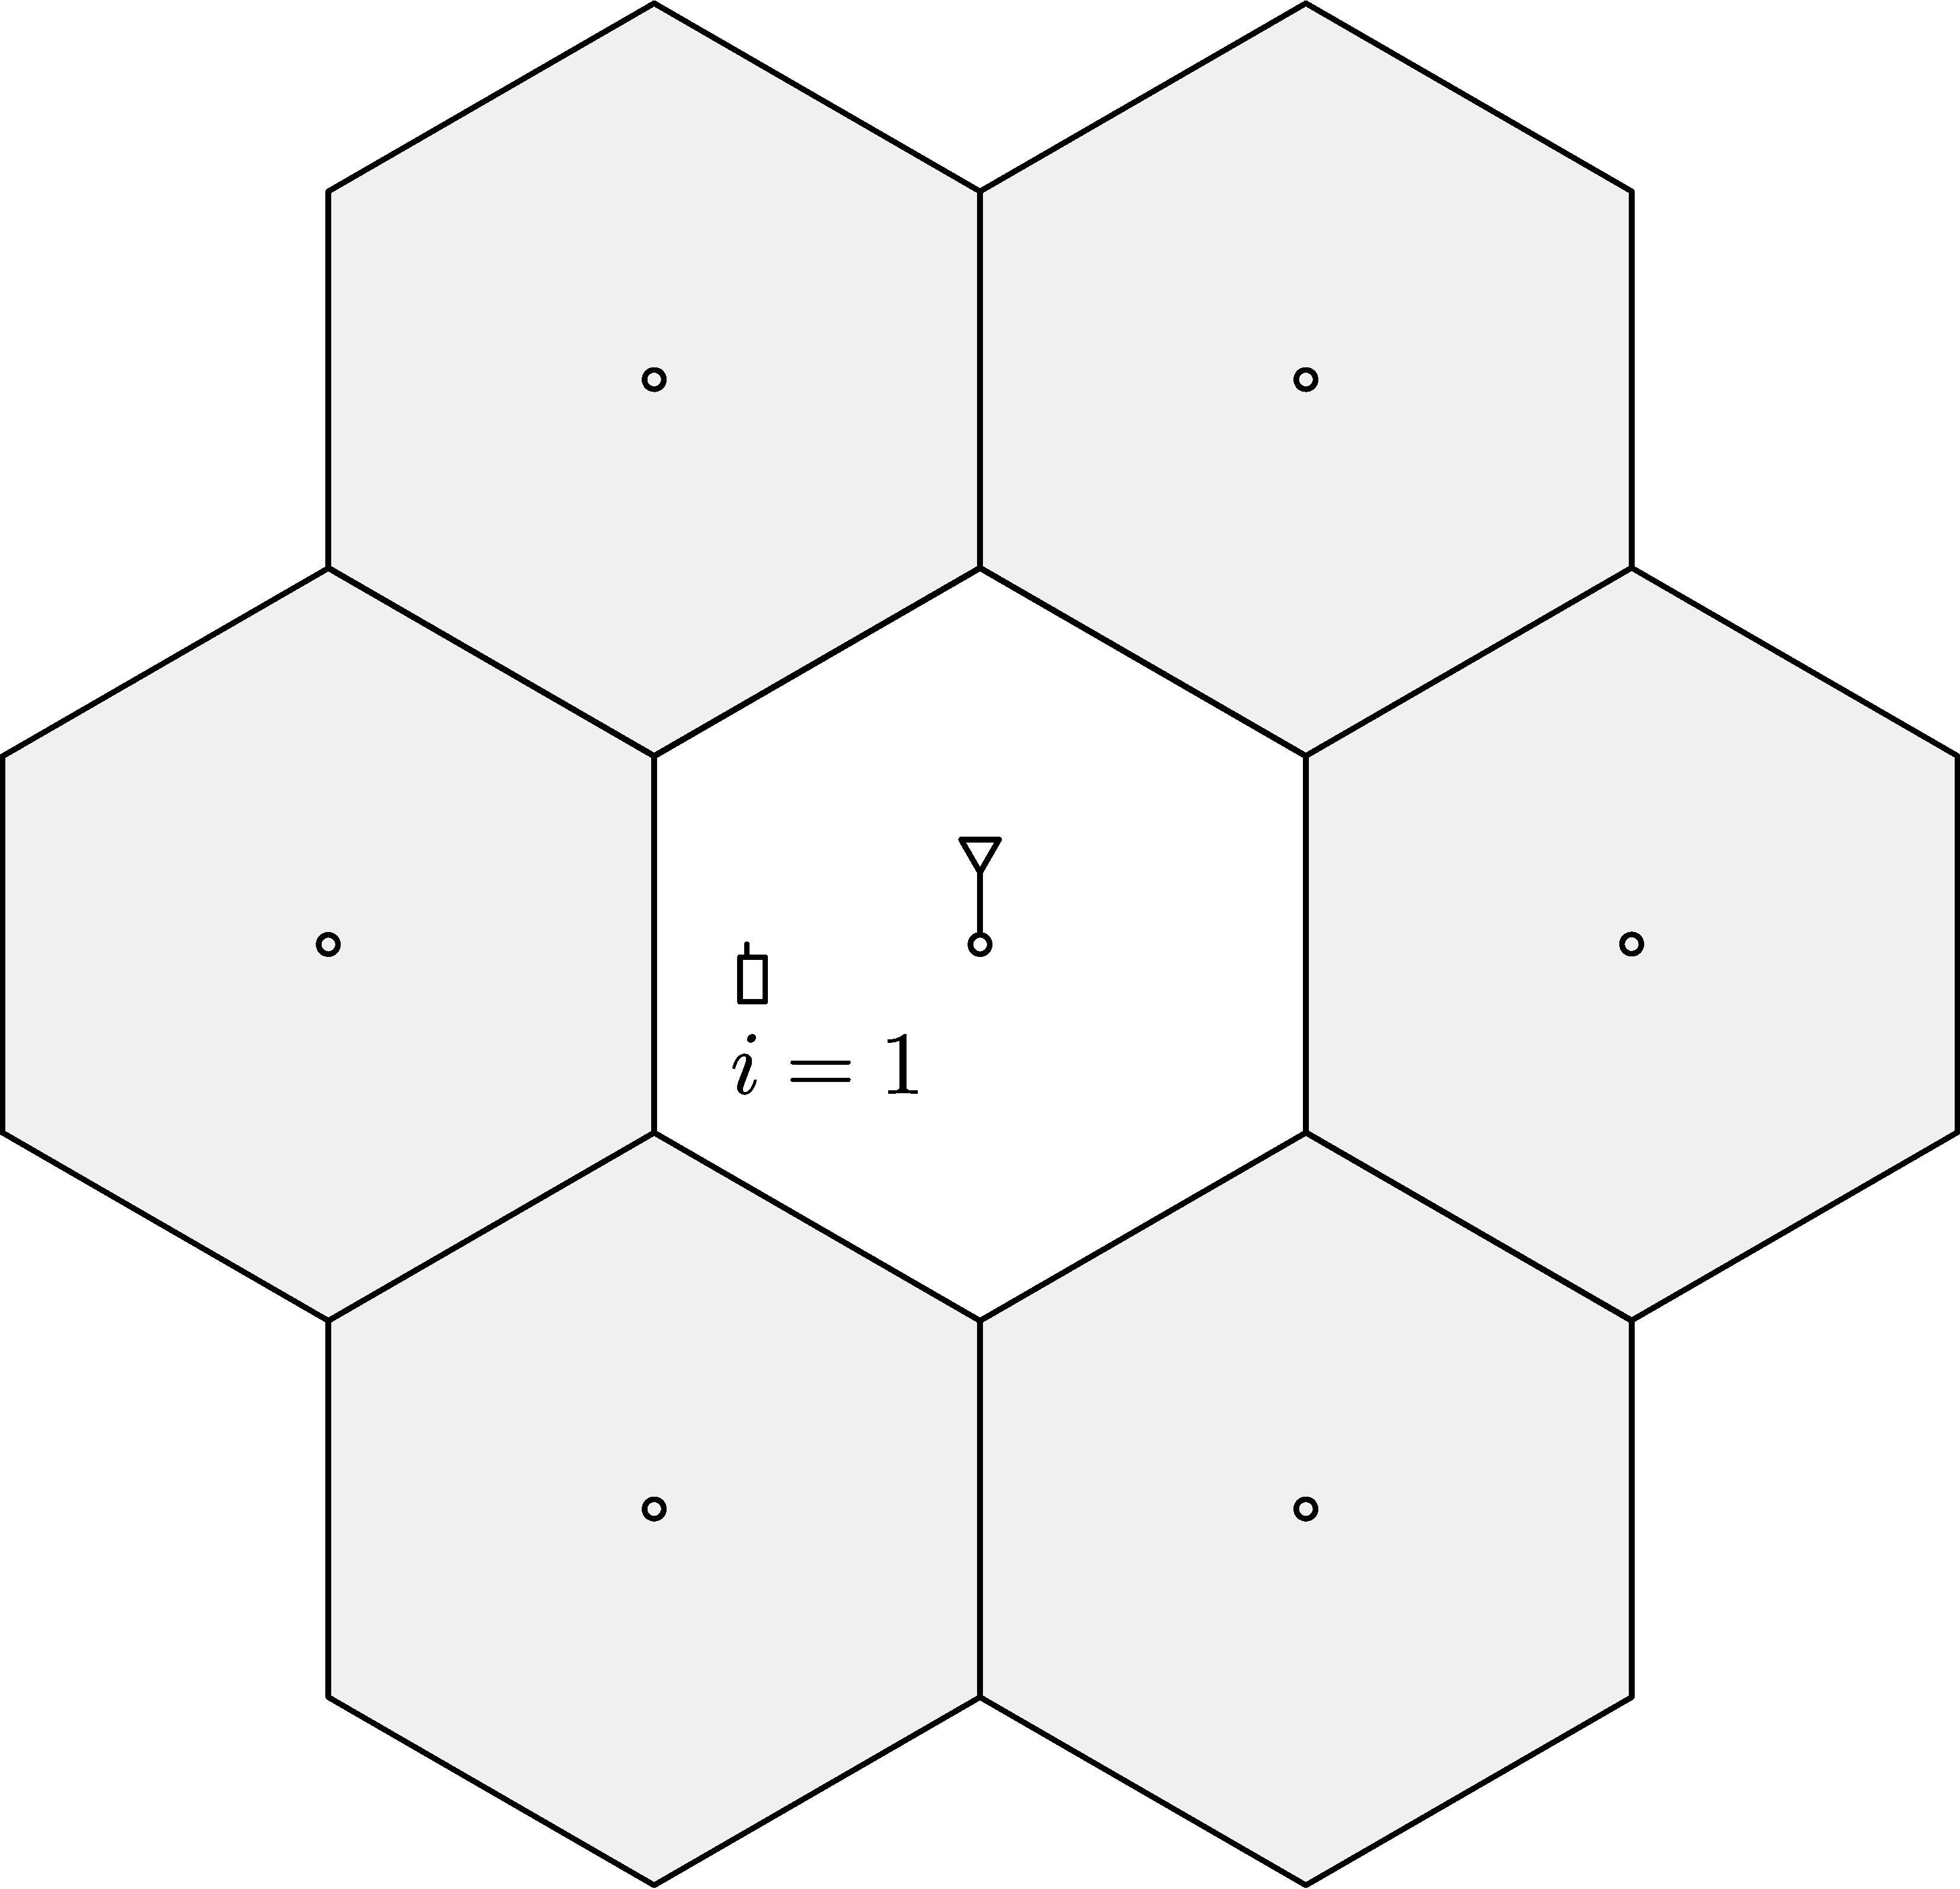
\includegraphics[width=0.8\textwidth]{./10.achievable_rates/img/cluster_1}
\end{center}
\caption{Simple scenario with a single cluster of $M = 1$ cell, and the six
    interfering cells surrounding it.}
\label{fig:cluster_1}
\end{figure}

An assumption that can be made is that half of the $M_{\text{int}, 1}$, \ie three, \glspl{bs} are located at a distance $\left( D_1 - d_1 \right)$ and the
other half are located at a distance $\left( D_1 + d_1 \right)$. Accordingly,
the interference power can be expressed as

\begin{equation} \label{eq:interf_cluster_1}
    I_1\left(d_1\right) = P_{\max} \left[ \frac{3}{\left(D_1 + d_1
        \right)^\gamma} + \frac{3}{\left(D_1 + d_1 \right)^\gamma}\right]
\end{equation}

\noindent
which is equal to \eqref{eq:interf_power_eq} if the equivalent number of
interfering \glspl{bs} is defined as

\begin{equation} \label{eq:meq_cluster_1}
    M_{\text{eq},1} = 3 \left[ 1 + \left(\frac{D_1 - d_1}{D_1 + d_1}
    \right)^\gamma\right]
\end{equation}

In general, if a user $i$ is considered to have $M_{\text{int}, i}$ interfering
\glspl{bs} in the first tier at a distance $D_i$, defined as in
\eqref{eq:interf_min_dist}, then the equivalent number of interfering \glspl{bs}
is given by

\begin{equation} \label{eq:general_meq}
    M_{\text{eq}, i} \approx \frac{M_{\text{int}, i}}{2} \left[ 1 + \left(
    \frac{D_i - d_i}{D_i + d_i}\right)^\gamma\right]
\end{equation}

In order to evaluate \eqref{eq:general_meq}, it is possible to set the distance
$d_i$ to the average distance of the user within the cell. A similar approach is
used in \cite{pijcke11} to characterize the statistics of the interference in a
multicell scenario. This average distance can be obtained from the uniform
spatial distribution in \eqref{eq:pdf_distance} as

\begin{equation} \label{eq:average_distance}
    \E\left\{d_i\right\} = \frac{2}{3}\Rcell
\end{equation}

\noindent
and then

\begin{equation} \label{eq:meq_cluster_generic}
    M_{\text{eq}, i} \approx \frac{M_{\text{int},i}}{2} \left[ 1 + \left(
        \frac{D_i - \frac{2}{3}\Rcell}
        {D_i + \frac{2}{3}\Rcell}\right)^\gamma\right]
\end{equation}

\refs{sec:achiev_numerical} deals with the comparison between simulations and
the analytical results, showing that the approximation in
\eqref{eq:meq_cluster_generic} is accurate.


%-------------------------------------------------------------------------------
\section{Analysis of the Rate}\label{sec:achiev_rate_analysis}

In the case of having global coordination or, equivalently, having only one
cluster including all the \glspl{bs}, the interference among the users is
completely eliminated through the use of \gls{bd}, \emph{cf.} \refs{sec:bd}. On
the other hand, in a multicluster environment, it is necessary to consider the
effect of the interference coming from the cells outside the cluster. Hence, the
mean achievable rate in \eqref{eq:bd_ergodic_capacity} becomes (dropping the
expectation notation)

\begin{equation} \label{eq:rate_bd_interf}
    R_i^{\text{BD}} = \sum\limits_{k = 1}^{\ell} \log_2 \left(1 +
        \frac{\lambdahat_{ik} p_{ik}}{\sigma_i^2 + I_i} \right)
\end{equation}

\noindent
where the parameter $I_i$ represents the average power of the total interference
contributions received in each data stream of user $i$ from the interfering
\glspl{bs}.

It can be seen in \eqref{eq:rate_bd_interf} that the rate depends on the distance $d_i$ of each user's equipment from the center of its cell. Using the pdf in
\eqref{eq:pdf_distance} the average of the rate over all possible locations,
making explicit the dependence on the distance $d_i$, can be expressed as

\begin{equation} \label{eq:rate_bd_loc_aver}
\begin{aligned}
    \bar{R}_i^{\text{BD}} &= \int\limits_0^{\Rcell} R_i^{\text{BD}}\left(u
    \right) \frac{2u}{\Rcell^2} \dee u \\
    &= \int\limits_0^{\Rcell} \sum\limits_{k = 1}^{\ell} \log_2 \left(1 +
    \frac{\lambdahat_{ik}\left(u\right) p_{ik}}{\sigma_i^2 + I_i\left(u\right)}
    \right) \frac{2u}{\Rcell^2} \dee u
\end{aligned}
\end{equation}

In \eqref{eq:rate_bd_loc_aver} there are three parameters that determine the
overall average rate, namely

\begin{itemize}
    \item The interference $I_i\left(d_i\right)$ coming from outside the
        cluster.
    \item The effect of the channel fading and of the path loss, represented by
        the term $\lambdahat_{ik}\left(d_i\right)$.
    \item The power $p_{ik}$ assigned to the $k$-th data stream of user $i$.
\end{itemize}

In the following, the characterization of each of these parameters will be
approached separatedly.

%-------------------------------------------------------------------------------
\subsection{Interference}\label{ssec:achiev_rate_interf}

As described in \refs{sec:achiev_interf} the contribution of interference,
$I_i\left(d_i\right)$ on each data stream of user $i$, coming from the cells
outside the cluster, can be considered as generated by an equivalent number of
\glspl{bs} located all of them at a distance of $D_i - d_i$ from the user.
Recall that, for clusters of size up to 18, $D_i$ can take one of two values as
in \eqref{eq:interf_min_dist}.

The interfering distance $D_i$ is then normalized to the cell radius $\Rcell$ by
setting

\begin{equation} \label{eq:interf_dist_norm}
    \bar{d}_i = \frac{D_i}{\Rcell}
\end{equation}

In expression \eqref{eq:rate_bd_interf} it is assumed that the interference can
be treated as Gaussian noise, so that the power is calculated as the variance
of that noise. Throughout the simulations that were performed, it has been found
that, on average, at least 25 out-of-cluster cells contributed with significant
interference.\footnote{Being significant defined as being greater than the power
received at the cell edge.}

This number of 25 is dependent on the simulation paremeters, but it gives an
idea of the order of magnitud of interferers present, and it justifies the
treatment of the interference as Gaussian noise, by virtue of the central limit
theorem \cite{papoulis_fourier}.

%-------------------------------------------------------------------------------
\subsection{Fading Effect}\label{ssec:achiev_rate_fading}

The terms $\lambdahat_{ij}$ are the squared diagonal values of the matrix
$\bLambdahat_i$, \emph{cf.} \refs{sec:bd}. This matrix is obtained in
\eqref{eq:svd_max_rate} by the combination of the channel matrix $\HH_i$ and a
unitary matrix, $\Vtilde_i^{(0)}$.

The channel matrix $\HH_i$ is composed of the submatrices $\HH_{ij}$, where the
fading elements have a power path loss of $d_{ij}^{-\gamma}$, and the elements
of $\HH_{ij}$ are independent from the elements of $\HH_{ik}$ for all $j$
different from $k$.

It is possible to define an alternative set of coefficients $\kappa_{ij}$ that
do not include the path loss effect

\begin{equation} \label{eq:kappa_coeff}
    \kappa_{ij} \triangleq \frac{\lambdahat_{ij}}{d_{i}^{-\gamma}}
\end{equation}

These coefficientes are the elements of the main diagonal of the matrix

\begin{equation} \label{eq:diag_matrix_no_path_loss}
    d_{i}^{\gamma}\bLambdahat_i \bLambdahat_i^H
\end{equation}

And it can be seen that these diagonal elements are the singular values of the
matrix

\begin{equation} \label{eq:wishart_mat}
    d_{i}^{\gamma}\HH_i\Vtilde_i^{(0)} \Vtilde_i^{(0),H} \HH_i^H
\end{equation}

\noindent
where $\HH_i$ has Gaussian entries, and $\Vtilde_i^{(0)}$ is a unitary matrix.

In the case of having $Mt = Nr$, the coefficientes $\kappa_{ij}$ are the
eigenvalues of a Wishart matrix while, in the general case of $Mt \geq Nr$ the
matrix in \eqref{eq:wishart_mat} can be approximated by a Wishart matrix.
Through simulations, it has been verified that the mean of the eigenvalues of 
both matrices, the original in \eqref{eq:wishart_mat} and the approximate
Wishart, is the same and the difference between the two \gls{cdf} is less than 10\,\%.

The joint \gls{pdf} of the eigenvalues $\kappa_{ij}$ of a Wishart matrix can be
obtained when the columns of the corresponding Gaussian matrix have an identity
covariance matrix

\begin{equation} \label{eq:cov_identity}
    \mathbf{\Sigma}_i = \eye
\end{equation}

\noindent
and it is given by \cite{tulino04}

\begin{equation} \label{eq:joint_pdf_eigenv_eye_cov}
    f_{\kappa_{i1}, \ldots, \kappa_{i\ell}}\left(\kappa_{i1}, \ldots,
    \kappa_{i\ell}\right) = e^{-\sum_{k=1}^{\ell}\kappa_{ik}}\prod_{k=1}^{\ell}
    \frac{1}{\left[\left(\ell - k\right)!\right]^2} \prod_{m = k + 1}^{\ell}
    \left(\kappa_{im} - \kappa_{i\ell}\right)^2
\end{equation}

However, in the evaluation of the rate the complete \gls{pdf} is not needed, and
only the sum

\begin{equation} \label{eq:sum_kappa}
    \sum_{i = 1}^{N}\sum_{k = 1}^{\ell} \log \left( \kappa_{ik} \right)
\end{equation}

\noindent
is required, which represents the expectation of the logarithm of the
determinant, for which results are available, also for the general case when the
covariance matrix is different from the identity, $\mathbf{\Sigma} \neq \eye$,
and it is given by \cite{tulino04}

\begin{equation} \label{eq:sum_log_kappa}
    \E\left\{\sum_{i=1}^{N}\sum_{k=1}^{\ell}\log\left(\kappa_{ik}
    \right)\right\} = \sum_{m = 1}^{N\ell} \psi\left(N\ell - m\right) +
    \log\left(\left|\mathbf{\Sigma}\right|\right)
\end{equation}

\noindent
where $\psi\left(\cdot\right)$ is the Euler's digamma function
\cite{gradshteyn00}, and where the matrix $\mathbf{\Sigma}$ is

\begin{equation} \label{eq:covariance_total}
    \mathbf{\Sigma} = \begin{bmatrix}
        \mathbf{\Sigma}_1 & \zero & \cdots & \zero \\
        \zero & \mathbf{\Sigma}_2 & \cdots & \zero \\
        \vdots & \vdots & \ddots & \vdots \\
        \zero & \zero & \cdots & \mathbf{\Sigma}_N
    \end{bmatrix}
\end{equation}

\noindent
with $\mathbf{\Sigma}_i$ the covariance matrix of the columns of the matrix
$d_{i}^{\sfrac{\gamma}{2}} \HH_i \Vtilde_i^{(0)}$

\begin{equation} \label{eq:covariance_not_eye}
    \mathbf{\Sigma}_i = \eye \left[1 + \sum\limits_{\substack{j=1\\j\neq i}}^{M}
        \left(\frac{d_{i}}{d_{ij}}\right)^{\gamma}
    \right]
\end{equation}

It is possible to define a parameter $G_i$

\begin{equation} \label{eq:cluster_gain}
    G_i \triangleq 1 + \sum\limits_{\substack{j=1\\j\neq i}}^{M} \left(
    \frac{d_{i}}{d_{ij}}\right)^{\gamma}
\end{equation}

\noindent
that can be considerd as a cluster gain. Its value can be approximated
considering the average distance of a user to its \gls{bs} 
\eqref{eq:average_distance}, and the distance from the rest of the \glspl{bs} in
the cluster to be either $\Dtone$ or $\Dttwo$. If additionally these two
distances are normalized by the average distance in \eqref{eq:average_distance}

\begin{equation} \label{eq:normalized_distances}
\begin{aligned}
    \Dtonebar &\triangleq \frac{3\Dtone}{2\Rcell} \\
    \Dttwobar &\triangleq \frac{3\Dttwo}{2\Rcell}
\end{aligned}
\end{equation}

\noindent
then the gain factor $G_i$ can be approximated for different cluster sizes as

\begin{equation} \label{eq:cluster_gain_value}
    G_i = \begin{cases}
    1 + \frac{M - 1}{2}\left[ \left( \frac{1}{\Dtonebar - 1}\right)^{\gamma}
    \left( \frac{1}{\Dtonebar + 1}\right)^{\gamma} \right]
    & M \leq 7 \\
    3 \left[ \left( \frac{1}{\Dtonebar - 1}\right)^{\gamma}
    \left( \frac{1}{\Dtonebar + 1}\right)^{\gamma} \right]
    \frac{M - 7}{2} \left[ \left( \frac{1}{\Dttwobar - 1}\right)^{\gamma}
    \left( \frac{1}{\Dttwobar + 1}\right)^{\gamma} \right]
    & 7 < M \leq 18
    \end{cases}
\end{equation}

In \reff{fig:sum_log_kappa} a fixed distance for the users equal to $d_{i} =
\sfrac{2}{3}\Rcell$, \eqref{eq:average_distance}, is considered and the values
of the sum of the natural logarithm of the values $\kappa_{ij}$ are calculated
through simulations and using the expression \eqref{eq:sum_log_kappa}, for the
case of $t = r = 2$.

\begin{figure}[t]
\begin{center}
%     \dummybox
    \hspace*{1mm}\input ./10.achievable_rates/img/Fig4.tex
\end{center}
\caption{Sum-log of the terms $\kappa_{ij}$. Comparison between simulations and
the values obtained using \eqref{eq:sum_log_kappa} for $ t = r = 2$.}
\label{fig:sum_log_kappa}
\end{figure}

It can be seen how the sum of the log values of $\kappa_{ij}$ presents a
diminishing increase as the cluster size $M$ increases. This can be explained by
a reduced contribution of the \glspl{bs}, that are farther than in smaller
clusters, which becomes negligible due to the path loss.

Notice that, in the evaluation of the mean achievable rate, a factor
$\sfrac{1}{N}$ is applied in order to evaluate the average rate per user, taking
into consideration that in a cluster with more cells, there would be more users
as well.

Thus, a decrease occurs in the mean achievable rate per user for large values of
$M$, as it will be shown in \refs{sec:achiev_numerical}.


%-------------------------------------------------------------------------------
\subsection{Power allocation}\label{ssec:achiev_rate_power}

Under the \gls{bd} strategy, the transmission within each cluster is equivalent
to a set of parallel non-interfering channels.

Therefore, the transmission power must be allocated in order to optimize some
quality of service parameters, such as the sum-rate or a weighted sum of the
rates, for the users of each cluster.

This objective is subject to a maximum transmission power available at each
\gls{bs}, \eqref{eq:pbpc_constraint} and \eqref{eq:trace_terms_p_i}

\begin{equation} \label{eq:pbpc}
	\sum\limits_{i = 1}^N \sum\limits_{k = 1}^\ell p_{ik} \left\| \wbar_{j, ik}
    \right\|_2^2 \leq P_{\max}
\end{equation}

\noindent
for each of the $M$ \glspl{bs} in the cluster.

The rate maximization problem is described in more detail in
\refs{sec:power_allocation}, and the solutions range from the simplest uniform
power allocation, \emph{cf.} \refss{ssec:uniform_allocation}, to an optimal
allocation, \emph{cf.} \refss{ssec:optimal_power_allocation}. In any case, the
problem of power allocation is not the focus of this work because it can be
solved separately and the actual powers could be inserted in the analytical
expressions developed.

Hence, in the following a theoretical framework is derived for the uniform power
allocation scheme, for the sake of simplicity, and an example with a different
power allocation will be presented with the results.

With a uniform power allocation a common average power $p_s$ is used for every
stream of every user, as seen in \eqref{eq:equal_power}. This value $p_s$ varies
according to the number of \glspl{bs} in the cluster, decreasing for a larger
size of the cluster, since a fraction of the overall available power is spent in
the coordination, to null the interference.

Substituting all the $p_{ik}$ in \eqref{eq:pbpc} by the common value $p_s$ it is
easy to see that the condition in \eqref{eq:pbpc} is limited by the \gls{bs} for
which the following factor is maximum

\begin{equation} \label{eq:chi_squared_j}
    \chi_j \triangleq \sum\limits_{i = 1}^N \sum\limits_{k = 1}^\ell \left\|
    \wbar_{j, ik} \right\|_2^2
\end{equation}

Assuming that the coefficients of the precoding matrix, \ie the elements
of the vector $\wbar_{j, ik}$, are Gaussian then $\chi_j$ is a Chi-squared
random variables with $\Np \triangleq N\ell t$ degrees of freedom, and then
the power $p_s$ is related to the reciprocal value of the maximum of $M$ random
variables

\begin{equation} \label{eq:ps_reciprocal}
    p_s = \frac{P_{\max}}{\E\left\{\chi\right\}}
\end{equation}

\noindent
with

\begin{equation} \label{eq:chi_squared}
    \chi = \max\left\{\chi_1, \ldots, \chi_M\right\}
\end{equation}

Then the probability distribution function of $\chi$ is given by

\begin{equation} \label{eq:chi_squared_dist_function}
    F_{\chi}\left(x\right) = P\left(\Np, x\right)^M
\end{equation}

\noindent
where $P\left(\cdot,\cdot\right)$ is the regularized Gamma function.

The mean value can be derived from the probability distribution function in
\eqref{eq:chi_squared_dist_function} as

\begin{equation} \label{eq:chi_squared_mean}
    \E\left\{\chi\right\} = \int\limits_0^\infty \left( 1 - F_{\chi}
    \left(x\right)\right) \dee x
\end{equation}

\noindent
and it can be bounded using

\begin{equation} \label{eq:bound_reg_gamma}
    \left(1 - e^{-\alpha x}\right)^a \leq P\left(a,x\right) \leq
    \left(1 - e^{-\beta x}\right)^a
\end{equation}

\noindent
with

\begin{equation} \label{eq:bound_parameters}
\begin{aligned}
    \alpha &= \begin{cases}
    1 & 0 < a < 1 \\
    \Gamma\left(a + 1\right)^{-\frac{1}{a}} & a > 1
    \end{cases} \\
    \beta &= \begin{cases}
    \Gamma\left(a + 1\right)^{-\frac{1}{a}} & 0 < a < 1 \\
    1 & a > 1
    \end{cases}
\end{aligned}
\end{equation}

\noindent
where $\Gamma\left(\cdot\right)$ is the Gamma function.

The average value of $\chi$ is then bounded by

\begin{equation} \label{eq:bound_chi}
    \frac{1}{\beta}\left[\psi\left(Mt + 1\right) + \gamma_0\right] \leq
    \E\left\{\chi\right\} \leq
    \frac{1}{\alpha}\left[\psi\left(Mt + 1\right) + \gamma_0\right]
\end{equation}

\noindent
with $\psi\left(\cdot\right)$ again the Euler's digamma function, and $\gamma_0$ the Euler-Mascheroni
constant.

It is possible to rewrite \eqref{eq:bound_chi} in terms of $p_s$ as

\begin{equation} \label{eq:bound_chi_ps}
    P_{\max} \frac{\Gamma\left(\Np + 1\right)^{-\frac{1}{\Np}}}
        {\psi\left(Mt + 1\right) + \gamma_0} \leq p_s \leq
        P_{\max}\frac{1}{\psi\left(Mt + 1\right) + \gamma_0}
\end{equation}

In the evaluation of the rate, the lower bound in \eqref{eq:bound_chi_ps} will
be considered, providing a lower bound to the average rate of each user.

The bounds for the power per stream $p_s$ in \eqref{eq:bound_chi_ps} are
compared in \reff{fig:bound_chi} with the results obtained through simulations.

\begin{figure}[t]
\begin{center}
%     \dummybox
    \hspace*{-0mm}\input ./10.achievable_rates/img/Fig5.tex
\end{center}
\caption{Normalized average power per stream $p_s / P_{\max}$ for different
antenna configurations: comparison between simulations and the bounds in
\eqref{eq:bound_chi_ps}.}
\label{fig:bound_chi}
\end{figure}

First thing that can be seen in \reff{fig:bound_chi} is how the power $p_s$
decreases with the size of the cluster, and this affects the mean achievable
rate as it will be discussed in \refs{sec:achiev_numerical}.

Secondly, \reff{fig:bound_chi} shows a very good agreement between the
analytical and simulation results for different antenna configurations. In
particular, the upper bound is tight for small clusters while the lower bound
becomes more accurate for bigger clusters.

%-------------------------------------------------------------------------------
\subsection{Evaluation of the mean achievable rate}\label{ssec:achiev_rate_eval}

The performance of the coordination scheme will be measured by the mean
achievable rate per user in the cluster

\begin{equation} \label{eq:mean_achiev_rate_def}
    \bar{R}^{\text{BD}} = \frac{1}{N} \sum\limits_{i = 1}^N
    \bar{R}_i^{\text{BD}}  
\end{equation}

It is possible to derive a lower bound for each user's average rate in
\eqref{eq:rate_bd_loc_aver} by considering the inequality

\begin{equation} \label{eq:log_ineq}
    \log\left(1+x\right) \geq \log\left(x\right)
\end{equation}

\noindent
so that the average rate for the $i$-th user \eqref{eq:rate_bd_loc_aver} becomes

\begin{equation} \label{eq:rate_bd_i_logapprox}
    \begin{aligned}
    \bar{R}_i^{\text{BD}} &\geq \frac{1}{\log\left(2\right)} \sum\limits_{k = 1}
    ^{\ell} \int\limits_0^{\Rcell} \log\left(\frac{p_{ik}\kappa_{ik}u^{-\gamma}}
    {\sigma_i^2 + P_{\max}\Meqi\left(D_i - u\right)^{-\gamma}}\right)\frac{2u}
        {\Rcell^2}\dee u \\
        &=\frac{1}{\log\left(2\right)}\sum\limits_{k=1}^{\ell}\left\{\log\left(
    \kappa_{ik}\right) + \log\left(\frac{p_{ik}}{P_{\max}}\right) + Z_i
    \right)
    \end{aligned}
\end{equation}

\noindent
where the interference model has been introduced, and $Z_i$ is defined as

\begin{equation} \label{eq:zi_def}
    Z_i \triangleq \int\limits_0^{\Rcell}\log\left(\frac{u^{-\gamma}}
        {\frac{\sigma_i^2}{P_{\max}} + \Meqi\left(D_i - u\right)^{-\gamma}}
    \right)\frac{2u}{\Rcell^2} \dee u
\end{equation}

The value of $Z_i$is derived in \refa{ch:appendix_a}, and it is

\begin{equation} \label{eq:zi_chapter}
\begin{aligned}
    Z_i &= \frac{\gamma}{2} + \log\left(\rho\right) + \bar{d}_i^2\log\left(
    \frac{\bar{d}_i^{\gamma}}{\Meqi \rho + \bar{d}_i^{\gamma}}\right)\\
    &- 2 \bar{d}_i^2\gamma \hgeo \left(1,\frac{1}{\gamma};
    \frac{\gamma+1}{\gamma};\frac{-\bar{d}_i^{\gamma}}{\Meqi\rho +
    \bar{d}_i^{\gamma}}\right)\\
    &+ \frac{\bar{d}_i^2}{2}\gamma \hgeo\left(1, \frac{2}{\gamma};
    \frac{\gamma+2}{\gamma};\frac{-\bar{d}_i^{\gamma}}{\Meqi\rho +
    \bar{d}_i^{\gamma}}\right)\\
    &- \left(\bar{d}_i^2-1\right)\log\left(
    \frac{\left(\bar{d}_i-1\right)^{\gamma}}
    {\Meqi\rho+\left(\bar{d}_i - 1\right)^{\gamma}}\right)\\
    &+ 2\bar{d}_i\left(\bar{d}_i - 1\right)\gamma\hgeo\left(1,\frac{1}{\gamma};
    \frac{\gamma + 1}{\gamma};\frac{-\left(\bar{d}_i-1\right)^{\gamma}}
    {\Meqi\rho}\right)\\
    &- \frac{\left(\bar{d}_i-1\right)^2}{2}\gamma\hgeo\left(1,\frac{2}{\gamma};
    \frac{\gamma + 2}{\gamma};\frac{-\left(\bar{d}_i-1\right)^{\gamma}}
    {\Meqi\rho}\right)
\end{aligned}
\end{equation}

\noindent
where $\hgeo\left(\cdot\right)$ is the hypergeometric function, and $\rho$ is
the \gls{snr} as defined in \eqref{eq:snr_noise}.

Combining \eqref{eq:sum_log_kappa}, \eqref{eq:bound_chi_ps},
\eqref{eq:mean_achiev_rate_def}, and \eqref{eq:rate_bd_i_logapprox} the
analytical expression for the mean achievable rate per user is

\begin{equation} \label{eq:mean_achiev_rate}
\begin{aligned}
    \bar{R}^{\text{BD}} &\geq \frac{1}{N\log\left(2\right)}
    \left[ \log\left(\left|\mathbf{\Sigma}\right|\right) +
    \sum\limits_{m=1}^{N\ell}\psi\left(N\ell-m\right) \right.\\
    &+N\ell \log\left(\frac{\Gamma\left(\Np + 1\right)^{-\frac{1}{\Np}}}
    {\psi\left(Mt + 1\right) + \gamma_0}\right)+\ell \left.
    \sum\limits_{i=1}^N Z_i\right]
\end{aligned}
\end{equation}

%-------------------------------------------------------------------------------
\section{Numerical Results}\label{sec:achiev_numerical}

In this section, the results derived from the analytical expression in
\eqref{eq:mean_achiev_rate} are compared with the results obtained through
simulations.

The scenario for the simulations is a network composed of 169 cells, laid out as
7 concentric tiers of hexagonal cells \reff{fig:simulation_scenario_achiev}.

\begin{figure}[t]
\begin{center}
    \dummybox
% image with the 7 tiers in a hexagonal grid
\end{center}
\caption{Scenario used for the simulations, with 7 hexagonal tiers.}
\label{fig:simulation_scenario_achiev}
\end{figure}

The cell radius, unless stated otherwise, is assumed to be $\Rcell=1.4$\,km.

All the results are averaged over 5,000 random trials. In each of these trials
the position of the users was randomly set according to a uniform distribution
inside each cell, \refs{sec:achiev_interf}. Also, for each of the trials, a
random channel was generated according to the model described in
\refs{sec:channel_model}, with a path loss exponent of $\gamma=3.8$.

The parameter evaluated in the simulations is the achievable rate defined in
\eqref{eq:rate_bd_interf}, in which the different variables required
(transmission power, interference power, $\lambdahat_{ik}$, etc) were obtained
by simulations.

As it has already been mentioned, the clusters considered are static,
\ie they are fixed and do not change for all the simulations. Despite
this, not all the clusters must have the same shape for the same cluster size
$M$. In fact, in the simulations, the clusters were generated following a
heuristic approach that tries to group cells in a compact way, with a regular
shape, by minimizing the sum of the inter-cell distances, thus to avoid long
clusters. Note, however, that some values of $M$ do not allow for regular
clusters, \ie hexagonal, to be formed. \reff{fig:irregular_clusters}
shows an example of this situation, where not all the clusters have the same
shape.

\begin{figure}[t]
\begin{center}
    \dummybox
% image with the scenario and the clusters marked, but not all of them with
% the same shape
\end{center}
\caption{Irregular shaping of the clusters, due to the heuristic clustering
algorithm used.}
\label{fig:irregular_clusters}
\end{figure}

%-------------------------------------------------------------------------------
\subsection{Analytical and simulation results comparison}
\label{ssec:achiev_comparison_simulations}

In order to validate the analytical expression \eqref{eq:mean_achiev_rate},
first it is compared with the mean achievable rate simulated using \gls{bd} and,
although the analytical derivations did not consider it and for the sake of
completeness, the \gls{mmse} precoder described in \cite{shi11}.

The antenna configuration used for this first comparison is $r=t=2$, and also
different values of the \gls{snr}, as defined in \eqref{eq:snr_noise}, are used
so to observe the behaviour in different \gls{snr} regimes.

\begin{figure}[t]
\begin{center}
%     \dummybox
    \hspace*{-2mm}\input ./10.achievable_rates/img/Fig6.tex
\end{center}
\caption{Mean achievable rate per user as a function of the number of
cells in the cluster for $r=2$, $t=2$, variable values of \gls{snr},
$\gamma=3.8$.}
\label{fig:rate_vs_cluster_size}
\end{figure}

\reff{fig:rate_vs_cluster_size} shows the mean achievable rate as a function of
the cluster size $M$.

As expected, the \gls{mmse} approach outperforms the \gls{bd} strategy at low
\gls{snr}. On the other hand, for moderate values of the \gls{snr} \gls{bd} is
able to provide comparable, and even more favorable, results, thus showing that
the interference dominates over the noise for regimes other than the low
\gls{snr} regime.

A very good agreement between the theoretical result in
\eqref{eq:mean_achiev_rate} and the simulations is clear in
\reff{fig:rate_vs_cluster_size}, where also some variations can be seen in the
simulation results. This is mainly due to the variability of the cluster shape,
as seen in \reff{fig:irregular_clusters}, for different cluster sizes, and not
to a low number of simulations that were averaged. That irregular shape of the
clusters, despite being more or less controlled in the heuristic
cluster selection algorithm, affects the simulation results in the form of the
variability shown in the figures.

\cite{lozano13} points out at a fundamental limit of cooperation, and it is
shown how the gains from cooperation cannot be unbounded, and that increasing
the number of coordinated elements may saturate the performance achieved. This
very same behaviour can be observed in \reff{fig:rate_vs_cluster_size}, both for
\gls{bd} and \gls{mmse}, where the mean achievable rate do not grow unboundedly
with the cluster size, and an optimum value of the size $M$ can be found.

\reff{fig:rate_vs_snr_gamma} also shows a similar behaviour. In this case, the
mean achievable rate is represented as a function of the \gls{snr}, and there is
an \gls{snr} at which the rate stops growing. This threshold \gls{snr} depends
on the propagation path loss exponent $\gamma$ because it directly determines
the influence of the interference. In particular, the saturation \gls{snr} for
\gls{bd} is higher than for \gls{mmse}. For the former, it is always above
20\,dB, for the scenarios considered, even for very small path loss exponents.
This means that the saturation occurs for relatively large values of the
\gls{snr} which is of practical importance because it would be possible to
deliver good performance, using \gls{bd}, within a practical range of \gls{snr}
values.

\begin{figure}[t]
\begin{center}
%     \dummybox
    \hspace*{-2mm}\input ./10.achievable_rates/img/Fig7.tex
\end{center}
\caption{Mean achievable rate as a function of the \gls{snr} for different
values of the path loss coefficient $\gamma$.}
\label{fig:rate_vs_snr_gamma}
\end{figure}

Under the restriction that the same $P_{\max}$ is transmitted for all values of
$\gamma$, the saturation occurs at different levels for each $\gamma$, although
the general conclusions do not change.

In order to complete the validation of the theoretical results with the
simulations, a fixed value of \gls{snr}$=25$\,dB and different antenna
configurations were considered in \reff{fig:rate_vs_size_antenna}, still using
uniform power allocation. The discrepancies between the theoretical results and
the simulations are not only due to the approximations, but also to the fact
that in the simulation scenario not all the clusters have the same shape,
despite having the same number of cells.

\begin{figure}[t]
\begin{center}
%     \dummybox
    \hspace*{0.5mm}\input ./10.achievable_rates/img/Fig8.tex
\end{center}
\caption{Mean achievable rate per user as a function of the cluster size for
\gls{snr}$=25\,$dB, $\gamma=3.8$ and different antenna configurations.}
\label{fig:rate_vs_size_antenna}
\end{figure}

%-------------------------------------------------------------------------------
\subsection{Effect of the power allocation}\label{ssec:achiev_power_allocation}

The cause of the decrease of the rate with respect to the cluster size, as seen
in \reff{fig:rate_vs_cluster_size}, is two-fold:

\begin{itemize}
    \item First, the value of the attenuation experienced by each data stream,
        $\lambdahat_{ik}$ decreases when the size of the cluster increases, as
        shown in \reff{fig:sum_log_kappa}.
    \item Second, the power assigned to each data stream, the terms $p_{ik}$
        that for a uniform power allocation are all equal to $p_s$, also
        decreases as the the cluster grows, \reff{fig:bound_chi}, due to a
        coordination ``loss''.
\end{itemize}

In this section, a different power allocation scheme, other than the uniform,
was used in order to verify if the behavior observed in
\reff{fig:rate_vs_cluster_size}, where the rate decreases with the cluster size,
is due to the power allocation.

The optimal power allocation used was obtained by means of numerical
optimization, as described in \cite{armada11b}, using CVX \cite{cvx},
\cite{gb08}, and those powers were plugged into \eqref{eq:mean_achiev_rate}
instead of the uniform power allocation.

\begin{figure}[t]
\begin{center}
%     \dummybox
    \hspace*{-1mm}\input ./10.achievable_rates/img/Fig9.tex
\end{center}
\caption{Comparison between different power allocation schemes, namely uniform
and optimal. Mean achievable rate per user as a function of the cluster size for
$r=t=2$, $\gamma=3.8$ and different values of \gls{snr}.}
\label{fig:rate_vs_size_power}
\end{figure}

In \reff{fig:rate_vs_size_power} the rates obtained with the uniform and the
optimum power allocation are compared and represented versus the size of the
cluster.

Although, as expected, the optimal outperforms the uniform power allocation,
both curves show a similar trend, meaning that a reduced growth of the rate (and
in some situationes a reduction of the rate itself) is not due to the power
allocation scheme, but it is the manifestation of a fundamental limitation of
the coordination scheme, along the lines of the results in \cite{lozano13}.

%-------------------------------------------------------------------------------
\subsection{Optimum cluster size}\label{ssec:achiev_optimum_size}

\reff{fig:rate_vs_cluster_size} through \reff{fig:rate_vs_size_power} show a
common trend which is the rate having a reduced growth, or even a reduction,
with the cluster size.

Given this, it is possible and interesing to find the cluster size $M$ that can
maximize the mean achievable rate.

In the case of the rate actually decreasing with $M$, the optimum value can be
readily obtained as the value of $M$ for which the maximum rate is obtained.

In some of the simulations results, the rate does not decrease within the range
of cluster sizes that were simulated, so it is not possible, with the simulation
conditions used, to find a maximum for the mean achievable rate. Something that
can be observed, nevertheless, is that its growth with $M$ is diminished so that
the optimum value of $M$ can be calculated by considering the relative change of
the rate. The optimum is assumed to be found when the marginal increase of the
rate is bellow a given percentage. In the case under study, the threshold was
set to a 10\,\%.

\begin{figure}[t]
\begin{center}
%     \dummybox
    \hspace*{-1mm}\input ./10.achievable_rates/img/Fig10.tex
\end{center}
\caption{Optimum cluster size as a function of the \gls{snr}, $\gamma=3.8$ and
different antenna configurations.}
\label{fig:optimum_M}
\end{figure}

\reff{fig:optimum_M} represents the optimum value of $M$ as a function of the
\gls{snr}, for different antenna configurations, and for the power allocation
schemes considered until now, uniform and optimum.

It can be seen that, for a wide range of \gls{snr}, the optimum value is limited
to around 7--10 cells.

Only for high \gls{snr} is it more convenient to increase the cluster size,
since the reduction of the interference can compensate the decrease of the
cluster gain due to the decrease of the factors $\lambdahat_{ik}$. This only
happens for the case of considering the optimal power allocation, because in the
case of the uniform power scheme there is the additional decrease of the power
allocated to each stream, $p_s$.

%-------------------------------------------------------------------------------
\subsection{Effect of signalling overhead}\label{ssec:achiev_signal_overhead}

It is common in the literature to not take into account the effect of the
signalling overhead, and the same has been done in all the previous results of
this work.

However, if a certain percentage of the available resources are dedicated to
channel estimation and control signalling, the effective \gls{snr} and the
payload that can be delivered are reduced with respect to the global achievable
rate.

In \cite{lozano13} the overhead, incurred by channel estimation requirements, is
accounted for by a percentage $\alpha$ which should grow, at least, linearly
with the cluster size, up to a maximum value, to prevent it from being greater
than 100\,\%. In that work, the \gls{snr} and the rate were effectively reduced
by a factor of $\alpha$, getting $\mathtt{SNR}_{\text{eff}}=\left(1-\alpha
\right)\mathtt{SNR}$ and $R_{\text{eff}} = \left(1-\alpha\right)R$.

\begin{figure}[t]
\begin{center}
%     \dummybox
    \hspace*{-1mm}\input ./10.achievable_rates/img/Fig11.tex
\end{center}
\caption{Mean achievable rate and payload rate as a function of the cluster size
$M$ with different SNRs.}
\label{fig:signal_overhead}
\end{figure}

In order to show the effect of the overhead on the achievable rate, in
\reff{fig:signal_overhead} a very conservative approach is adopted, in which the value of the reduction factor $\alpha$ scales linearly with the cluster size
$M$, up to a maximum of 10\,\% for a cluster size of 19.

\reff{fig:signal_overhead} shows the comparison of considering and not
considering the overhead. It can be seen that even with a small amount of
overhead, increasing values of $M$ lead to a worse performance.

Moreover, it should be stressed that the actual definition of signalling
overhead and its management is usually delegated to the operator implementation,
and this is seldom defined in the standards. Thus, its quantitative effect can
change considerably depending on how the overhead is defined.






% Rate statistics
\chapter[Rate Statistics]{Achievable Rate and Fairness in Coordinated Base
Station Transmission\footnote{The work shown in this chapter has been published
in \cite{corvaja14}.}}\label{ch:rate_statistics}

% ------------------------------------------------------------------------------
\section{Introduction}\label{sec:stats_intro}

\refc{ch:achiev_rates} deals with the evaluation of the mean achievable rate,
and the analysis of the influence of the cluster size and power assignment on
the maximization of the rate. This chapter in turn focuses on the analysis of
the \gls{qos} of the system, in terms of the fairness in the distribution of the
achievable rate among the users.

Although the mean achievable rate, as calculated in \refc{ch:achiev_rates} can
provide useful information, also the \gls{cdf} plays an important role when
designing fairness, and other \gls{qos} related, management strategies in
coordinated downlink networks.

In the following, it is shown that the statistics of the achievable rate are
almost perfectly represented by a Gamma distribution. Note that the Gamma
distribution arises in several contexts when considering non-negative random
variables whose value is determined by several joint distributions. For example,
in \cite{heath13} it is used to model the interference in an
interference-limited cellular network in order to simplify the calculation of
the success probability, \ie the complementary event of an outage, and
the ergodic rate. In \cite{alahmadi10} a Gamma distribution is used to model
composite fading channels. And in \cite{atapattu11} a mixture Gamma distribution
is proposed to describe the \gls{snr} of wireless channels, mainly composite
shadowing/fading channels, but also many other small-scale fading channels.

This chapter provides a characterization of the \gls{cdf} of the achievable rate
in a coordinated base station transmission with \gls{bd}, where the \glspl{bs}
are grouped in clusters and the interference is due to adjacent clusters.

Using the system model from \refc{ch:system_model}, including the power
assignment strategies described there, and the cluster model proposed in
\refs{sec:achiev_clust_net}, the dependence of the \gls{cdf} on the cluster
size, and the power assignment strategy is studied as well in the current
chapter.

% ------------------------------------------------------------------------------
\section{Rate Statistics}\label{sec:stats_rate_stats}
% ------------------------------------------------------------------------------
\subsection{Cumulative Distribution Function}\label{ssec:stats_cdf}

Recal the expression of the achievable rate when \gls{bd} is used to coordinate
the \glspl{bs} in the cluster

\begin{equation} \label{eq:stats_achiev_rate}
    R_i^{\text{BD}}\left(d_i\right) = \sum\limits_{k = 1}^{\ell} \log_2 \left(
    1 + \frac{\lambdahat_{ik} p_{ik}}{\sigma_i^2 + I_i\left(d_i\right)} \right)
\end{equation}

\noindent
where the dependence on the $i$-th user's distance to its \gls{bs}, $d_i$, is
made explicit, the interference power is defined by \eqref{eq:interf_power}, the
noise power $\sigma_i^2$ is obtained as a function of the \gls{snr} using
\eqref{eq:snr_noise}, and the powers $p_{ik}$ would be computed using the power
allocation strategies described in \refs{sec:power_allocation}.

The derivation of the complete statistical characterization of the achievable
rate per user is an almost intractable task, due to the combination of many
effects such as the power assignment, the interference coming from outside the
cluster, the channel characteristics, etc. Even the evaluation of the mean
requires to resort to several approximations, although the final result has been
shown to be quite accurate, \emph{cf.} \refc{ch:achiev_rates}.

If the \gls{pdf} of the achievable rate per user is considered, a suitable
analytical model is provided by the Gamma distribution's \gls{pdf}

\begin{equation} \label{eq:gamma_pdf}
   f_{R}\left(x\right) = \frac{1}{\Gamma\left(\theta\right)\theta^k}x^{k-1}
   e^{-\frac{x}{\theta}}
\end{equation}

\noindent
with mean and variance given by $k\theta$ and $k\theta^2$, respectively, and
related to the system parameters as discussed in \refss{ssec:stats_mean} and
\refss{ssec:stats_variance}.

The choosing of the Gamma distribution is not arbitrary, and it is motivated by
the fact that the achievable rate per user in \eqref{eq:stats_achiev_rate} is
the result of adding several non-negative terms. The \emph{central limit theorem
for causal functions} \cite{papoulis_fourier} states that the convolution of an
unbounded number of causal functions can be approximated using a Gamma
distribution. A causal function is a function defined only for $\R^{+}
\cup \left\{0\right\}$, as $\log_2\left(1+x\right)$ with $x \geq 0$ is. In the
case under study the sum of terms is not unbounded, but \cite{papoulis_fourier}
shows also how the approximation is accurate also for a sum of a finite number
of terms.

The Gamma distribution has been introduced also in \cite{cheikh11} to describe
the \gls{sir} in a simpler environment, without noise and without any kind of
coordination.

In fact, when comparing the CDF obtained by simulation and a Gamma \gls{cdf},
with the same mean and variance, it is interesting to note a very accurate
fitting.

\begin{figure}[t]
\begin{center}
%     \dummybox
    \newgeometry{textwidth=0.7\textwidth}
    \input ./11.rate_statistics/img/cdf_gamma_tikz.tex
    \restoregeometry
\end{center}
\caption{\gls{cdf} of the achievable rate per user with $r=2$, $t=2$, and
SNR=15\,dB. Comparison with the Gamma distribution with the same mean and
variance.}
\label{fig:cdf_sim_analy}
\end{figure}

\reff{fig:cdf_sim_analy} shows the perfect match between the experimental
\gls{cdf} and a Gamma \gls{cdf} for a uniform power allocation, and for
different system parameters.

The effect of increasing the size of the cluster on the \gls{cdf} of the
achievable rate is shown in \reff{fig:cdf_cluster_size}

\begin{figure}[t]
\begin{center}
%    \dummybox
    \newgeometry{textwidth=0.7\textwidth}
    \input ./11.rate_statistics/img/cdf_clusters_tikz.tex
    \restoregeometry
\end{center}
\caption{\gls{cdf} of the achievable rate per user with $r=2$, $t=2$, and
SNR=15\,dB for different values of the cluster size.}
\label{fig:cdf_cluster_size}
\end{figure}

\reff{fig:cdf_cluster_size} also shows how the rate increases with the cluster
size up to a certain point, and then it starts to decrease. This is the same
behavior observed in the mean achievable rate in \refc{ch:achiev_rates}.

Another aspect that can be seen is how the variance of the rate decreases as the
cluster size increases.

% ------------------------------------------------------------------------------
\subsection{Effect of the power allocation}\label{ssec:stats_power_alloc}

Three different power allocation schemes have been considered:

\begin{itemize}
   \item Uniform power allocation, as described in
      \refss{ssec:uniform_allocation}.
   \item The modified water-filling from \refss{ssec:modified_wf}.
   \item Power allocation result of solving the convex optimization
      problem \eqref{eq:sum_rate_maxim} using numerical solvers. In particular
      the numerical solver used is CVX \cite{cvx}, \cite{gb08}. For the rest of
      the chapter, this solution will be noted as CVX solution.
\end{itemize}

\begin{figure}[t]
\begin{center}
%    \dummybox
    \newgeometry{textwidth=0.7\textwidth}
    \input ./11.rate_statistics/img/cdf_gamma_power_tikz.tex
    \restoregeometry
\end{center}
\caption{\gls{cdf} of the achievable rate per user with $r=3$, $t=3$, and SNR=15\,dB.
Comparison between different power allocation schemes.}
\label{fig:cdf_power_alloc}
\end{figure}

In order to show the effect of using each of these power allocation schemes,
\reff{fig:cdf_power_alloc} presents the \gls{cdf} of the achievable rate per
user for the three of the schemes proposed, and using a constant antenna setup
of $t = r = 3$ antennas, an SNR=15\,dB, and two different cluster sizes, namely
$M \in \left\{5, 8\right\}$.

It should be noted that both the water-filling and the numerical solutions are
calculated for the problem formulated in \eqref{eq:sum_rate_maxim}, where no
out-of-cluster interference is present, so that these solutions are not adapted
to a multicluster environment. This is so because such adaptation would require
some sort of coordination among different clusters, and that is out of the scope
of this work.

% ------------------------------------------------------------------------------
\subsection{Mean value}\label{ssec:stats_mean}

The derivation of the mean value has been done in \refc{ch:achiev_rates}
resorting to some approximations that allow to evaluate the mean achievable rate
defined as in \eqref{eq:rate_bd_loc_aver}

\begin{equation} \label{eq:rate_bd_loc_aver_2}
    \bar{R}_i^{\text{BD}} = \int\limits_0^{\Rcell} R_i^{\text{BD}}\left(u
    \right) \frac{2u}{\Rcell^2} \dee u
\end{equation}

\noindent
using a particular model for the interference coming from outside the cluster,
\emph{cf.} \refs{sec:achiev_interf}.

The value of the mean that is thus obtained is rather accurate for a wide range
of the scenario parameters, as it is shown in detail in \refc{ch:achiev_rates}.

% ------------------------------------------------------------------------------
\subsection{Variance}\label{ssec:stats_variance}

A closed form expression for the variance of the achievable rate cannot be
obtained without too many simplifying approximations so, instead, an accurate
value is obtained through simulations.

\begin{figure}[t]
\begin{center}
%     \dummybox
    \newgeometry{textwidth=0.7\textwidth}
    \input ./11.rate_statistics/img/varianza_tikz.tex
    \restoregeometry
\end{center}
\caption{Variance of the achievable rate per user with different values of
\gls{snr} and of $t$ and $r$ as a function of the cluster size $M$.}
\label{fig:rate_variance}
\end{figure}

\reff{fig:rate_variance} shows the variance of the achievable rate per user as a
function of the cluster size $M$. The different curves are for different system
parameters, for instance, several values of the \gls{snr} and different antenna
configurations. Other simulation parameters are fixed, as is the path loss
exponent $\gamma=3.8$, which is a rather typical value for urban environments as
used in \cite{karakayali06}, and the uniform power assignment that is
considered.

It is interesting to note that increasing the degrees of freedom available in
the system, by using a higher number of antennas, increases the variance of the
achievable rate. Something similar happens when the \gls{snr} of the system
increases.

An important detail that can be stressed is how the variance does not decrease
unboundedly with the cluster size, but a minimum can be found, analogously to
the maximum that can be found in the mean achievable rate in
\refss{ssec:achiev_optimum_size}.

Understanding that fairness in the system is closely related to the variance of
the achievable rates per user, it is plain to see that in order to maximize the
fairness of the system, a limited number of \glspl{bs} per cluster is
preferable.

% ------------------------------------------------------------------------------
\section{Fairness and QoS considerations}\label{sec:stats_fairnes_qos}

Using the statistics of the coordination schemes considered that have been
presented in \refs{sec:stats_rate_stats}, several fairness and \gls{qos}
characteristics can be studied.

One of these is the minimum rate that can be guaranteed to a percentage $X$ of
the users. This is given by the value of the rate, the abscise, when the
\gls{cdf} is equal to $\left(1 - \sfrac{X}{100}\right)$, which gives the rate
that can be guaranteed to $X$\,\% of the users.

\begin{figure}[t]
\begin{center}
%     \dummybox
    \newgeometry{textwidth=0.7\textwidth}
    \input ./11.rate_statistics/img/fairness_90_tikz.tex
    \restoregeometry
\end{center}
\caption{Rate achieved by 90\,\% of the users with different antenna
configurations and different values of \gls{snr}.}
\label{fig:min_rate_sys_param}
\end{figure}

\reff{fig:min_rate_sys_param} presents the rate achieved by 90\,\% of the users
as a function of the cluster size $M$, for different system parameters,
considering a uniform power assignment.

The behavior observed suggests, again, that a limited cluster size is advisable
in order to deliver the advantages of \gls{mimo} to the maximum number of users
possible.

A maximum of the minimum rate guaranteed to 90\,\% of the users appears for a
cluster size of around 7, and it decreases as the cluster grows bigger. This
decrease is steeper for higher number of antennas because the variance
increases, as seen in \reff{fig:rate_variance}. In particular, it can be seen
that for clusters of size 18, a configuration with $t=r=4$ performs worse than a
configuration with $t=r=3$.

Note, however, that the power assignment method plays an important role, as it
can be seen from the slope of the \gls{cdf} in \reff{fig:cdf_power_alloc}. In
order to illustrate this, \reff{fig:min_rate_power_alloc} represents the minimum
rate that can be guaranteed to 90\,\% of the users for different power
allocation strategies.

\begin{figure}[t]
\begin{center}
%     \dummybox
    \newgeometry{textwidth=0.7\textwidth}
    \input ./11.rate_statistics/img/fairness_90_power_tikz.tex
    \restoregeometry
\end{center}
\caption{Rate achieved by 90\,\% of the users with different power assignment
schemes, $r=3$, $t=3$, and SNR$=15$\,dB.}
\label{fig:min_rate_power_alloc}
\end{figure}

The CVX power allocation scheme presents the worst performance, in terms of
the minimum guaranteed rate. It is easy to understand that the CVX solution
tries to maximize the sum-rate, which comes at the cost of letting the users
with the worst conditions out, yielding a very unfair system.

On the other hand, both waterfilling and the uniform assignment schemes perform
better in this regard, and they show a similar behavior. The only difference in
the behavior appears for bigger clusters. The uniform power assignment performs
better for small clusters, and the minimum rate decreases noticeably for large
clusters. The modified water-filling alternative shows a much more constant
behavior, with much less difference between small and big clusters.


% Scheduling
\chapter[Adaptive User Scheduling]{Adaptive Block Diagonalization and User
Scheduling With Out of Cluster Interference\footnote{The work shown in this
chapter has been presented in \cite{jjgarcia14}.}}\label{ch:adaptive_schedule}

% ------------------------------------------------------------------------------
\section{Introduction}\label{sec:sched_intro}

In \refc{ch:achiev_rates} and \ref{ch:rate_statistics} the performance of a
clustered network using \gls{bd} has been analyzed, both in terms of mean
achievable rate per user and in terms of network fairness. In both studies, a
common result appears: a limited cluster size can be beneficial. This is true
not only regarding the rate that the users can achieve, but also considering
the requirements imposed on the network infrastructure. When the size of the
cellular network grows, global coordination becomes impractical, due to the
increased feedback and backhaul requirements. Additionally, there are
theoretical works that show how the gains from coordination are intrinsically
limited for an increasing network size \cite{lozano13}.

The main drawback of clustering is the presence of \gls{oci}, and in particular
\gls{bd} performs poorly when \gls{oci} is considered \cite{shim08}. The problem
approached in this chapter is the performance loss of \gls{bd} when \gls{oci} is
present. A simple and practical algorithm is presented, based on a hybrid
strategy combining \gls{bd} and \gls{su} processing. The best transmission
strategy is chosen according to a metric that is compared with a simple
threshold at each user equipment.

The scenario here considered is a multiuser network, with each cell serving
multiple users. A low-complexity algorithm is proposed to schedule the users,
trying to take advantage of the multiuser diversity to increase the mean rate
per user. In \cite{shen06} a similar suboptimal algorithm, based on the
Frobenius norm of the channel matrix is proposed, but it is not analyzed in the
presence of \gls{oci} nor is it combined with a hybrid precoding strategy.

% ------------------------------------------------------------------------------
\section{System Model}\label{sec:sched_system_model}

The system model used in this chapter is the same as the clustered network model
in \refc{ch:achiev_rates}. It is focused on the downlink of a cellular network
with a set of $\B = \Bin \cup \Bout$ of cells, where $\Bin$ is the set of $M$
cells that form the cluster under study, $\Bout$ represents the set of
$\Minterf$ cells external to the cluster, and $\Bin \cap \Bout = \emptyset$.
Again, it will be considered that each user is associated to one and only one
\gls{bs}.

The signal received at the $i$-th user equipment is then given by

\begin{equation} \label{eq:yi_oci_present}
    y_i = \HH_i \Wtx_i \ss_i + \underbrace{\sum\limits_{\substack{j=1\\j\neq i}}
    ^{N} \HH_i \Wtx_j \ss_j}_{\text{Inner Interference}} +
    \underbrace{\sum\limits_{k \in \Bout} \Hbar_{ik} \xbar_k}_{\text{OCI}}
    + \nn_i
\end{equation}

\noindent
which is another way of writing \eqref{eq:rx_signal_user_interf} when external
interference is considered. $\Hbar_{ik} \in \C^{r \times t}$ is the channel
matrix from the $k$-th \gls{bs} outside the cluster to the $i$-th user in the
cluster, and $\xbar_k$ is the transmitted signal at the $k$-th \gls{bs} outside
the cluster.

Analogously to \eqref{eq:interf_plus_noise}, the interference and noise terms in
\eqref{eq:yi_oci_present} can be grouped together

\begin{equation} \label{eq:zi_hat}
    \zhat_i = \sum\limits_{\substack{j=1\\j\neq i}}^{N} \HH_i \Wtx_j \ss_j +
    \sum\limits_{k \in \Bout} \Hbar_{ik} \xbar_k + \nn_i.
\end{equation}

The ergodic rate obtained at the $i$-th receiver can then be written as

\begin{equation} \label{eq:rate_yi_oci}
    R_i = \log_2\left|\eye + \HH_i\Wtx_i\RR_{\ss_i}\WtxH_i\HH_i^H
    \RR_{\zhat_i}^{-1}\right|
\end{equation}

\noindent
where

\begin{equation} \label{eq:zhat_cov}
\begin{aligned}
    \RR_{\zhat_i} &= \E\left\{\zhat_i\zhat_i^H\right\} \\
    &= \sum\limits_{\substack{j=1\\j\neq i}}^{N} \HH_i \Wtx_j \RR_{\ss_j}
    \WtxH_j \HH_i^H + \sum\limits_{k \in \Bout} \Hbar_{ik} \RR_{\xbar_k} 
    \Hbar_{ik}^H + \sigma^2\eye
\end{aligned}
\end{equation}

\noindent
is the covariance matrix of the interference plus noise vector in
\eqref{eq:zi_hat}.

The rate expression \eqref{eq:rate_yi_oci} depends on the transmission strategy
used within the cells of the cluster, represented by the precoding matrix
$\Wtx_i$ for $i \in \Bin$. In the current work two transmission strategies are
considered:

\begin{itemize}
    \item Block Diagonalization.
    \item Single User Processing.
\end{itemize}

% ------------------------------------------------------------------------------
\section{Transmission Strategy} \label{ssec:sched_strategy}

% ------------------------------------------------------------------------------
\subsection{Block Diagonalization} \label{ssec:sched_bd}

\gls{bd} transmission strategy has been thoroughly described in \refs{sec:bd} in
the absence of interference coming from outside the cluster that is coordinated
using \gls{bd}.

In this work, \gls{oci} is considered, and in this case \gls{bd}
is not able to remove it, as the \glspl{bs} only coordinate to get rid of the
interference from within the cluster. As a result, the rate obtained when using
\gls{bd} is no longer given by \eqref{eq:bd_ergodic_capacity}, but the following
revised expression

\begin{equation} \label{eq:bd_rate_oci}
    R_{i}^{\text{BD}} = \log_2\left|\eye + \bLambdahat_i \RR_{\ss_i}
    \bLambdahat_i^H \left(\sum\limits_{k \in \Bout} \Hbar_{ik} \RR_{\xbar_k}
    \Hbar_{ik}^H + \sigma^2\eye\right)^{-1}\right|
\end{equation}

\noindent
where the additional term due to the \gls{oci} is present and $\RR_{\xbar_k} =
\E\left\{\xbar_k \xbar_k^H\right\} \in \C^{t \times t}$ is the covariance matrix
of the signal transmitted from the $k$-th \gls{bs} outside the cluster.

% ------------------------------------------------------------------------------
\subsection{Single User Processing} \label{ssec:sched_su}

The other transmission strategy that is considered in this work is Single User
processing. This is the case when no coordination is used, so that each \gls{bs}
serves only one user and, therefore, all the rest of \glspl{bs} are considered
interferers.

This translates into

\begin{equation} \label{eq:wtx_su}
    \Wtx_{ij} = \zero \forall j \neq i.
\end{equation}

The signal received at the $i$-th user can be written as

\begin{equation} \label{eq:yi_su}
    y_i = \HH_{ii}\xx_i + \underbrace{\sum\limits_{\ell \in \Bin \backslash
    \left\{i\right\}} \HH_{i\ell} \xx_{\ell}}_{\text{Inner Interference}} +
    \underbrace{\sum\limits_{k \in \Bout} \Hbar_{ik} \xbar_k}_{OCI} + \nn_i
\end{equation}

Provided \eqref{eq:yi_su}, if the \gls{svd} of the channel matrix $\HH_{ii}$ is
considered

\begin{equation} \label{eq:hi_svd}
    \HH_{ii} = \UU_i \Lambda_i \VV_i^H
\end{equation}

\noindent
then the following precoding matrix can be used in order to maximize the rate of
the $i$-th user \cite{telatar99}

\begin{equation} \label{eq:precod_su}
    \Wtx_{ii} = \VV_i
\end{equation}

\noindent
so that, using $\UU_i^H$ as the receive filter, the achievable rate becomes

\begin{equation} \label{eq:rate_su}
\begin{aligned}
    &R_i^{\text{SU}} = \\
    &\log_2\left|\eye + \bLambda_i \RR_{\ss_i} \bLambda_i^H \left(
    \sum\limits_{\ell \in \Bin \backslash \left\{i\right\}} \HH_{i\ell}
    \RR_{\xx_{\ell}} \HH_{i\ell}^H + \sum\limits_{k \in \Bout} \Hbar_{ik}
    \RR_{\xbar_k} \Hbar_{ik}^H + \sigma^2 \eye \right)^{-1} \right|
\end{aligned}
\end{equation}

% ------------------------------------------------------------------------------
\subsection{Transmission Strategy Selection} \label{ssec:sched_selection}

In \cite{zhang10} it is shown that the maximum capacity of a \gls{miso} downlink
channel can be reached using a combination of two transmission strategies, the
optimal \gls{mrt} and \gls{zfbf}. Based on this, \cite{moon13} presents a method
for the users to decide locally and individually the most convenient
transmission strategy from the two options presented in \cite{zhang10}. The way
to do this is through a threshold on the \gls{sinr}, and a closed form
expression for this threshold is provided in \cite{moon13}.

In \cite{zuleita09}, a similar result to that of \cite{zhang10} is presented for
the \gls{mimo} case, but the solution offered, apart from not having a closed
form expression, was based on sequentially solving a series of optimization
problems, which renders its applicability rather difficult.

In the current work, the same approach as in \cite{moon13} is followed. The
proposal is to use a metric that can be easily calculated at each receiver, and
to compare this metric with a fixed threshold locally at each user in order to
decide which transmission strategy to use.

Intuitively, \gls{bd} will perform better when the \gls{oci} is low, compared to
the power received from the \glspl{bs} in the cluster. Hence, the proposed
metric is

\begin{equation} \label{eq:metric}
   \theta_i =
   \frac{\sum\limits_{j \in \Bin} \Tr\left(\HH_{ij}\RR_{\xx_j}\HH_{ij}^H\right)}
   {\sum\limits_{k \in \Bout} \Tr\left(\Hbar_{ik}\RR_{\xbar_k}\Hbar_{ik}^H
   \right)}
\end{equation}

\noindent
which is the quotient of the power received from the \glspl{bs} in the cluster
and the power received from the \glspl{bs} outside the cluster.

After the metric is computed, it is compared with a fixed threshold
$\thetath$ for which there is no closed form expression. That is the
reason why the threshold considered in this work is calculated through
simulations and it is assumed to be known by all the users. The details of how
this threshold is calculated are given in \refs{sec:sched_performance}.

The decision about what transmission strategy to use is made locally by each
user. The $i$-th user compares the metric $\theta_i$ with the threshold
$\thetath$, and decides to use \gls{bd} if $\theta_i >
\thetath$, and choosen \gls{su} if $\theta_i \leq \thetath$.

All the users feed back their decissions to their \gls{bs}, and this information
is jointly used by the \glspl{bs} in the cluster to coordinate the scheduling of
the users and the transmission strategy used for each of them.

% ------------------------------------------------------------------------------
\section{Scheduling}\label{sec:sched_scheduling}

After the users have made their decision and fed it back to the \glspl{bs},
these will know which users are more suited to being served using \gls{bd} and
which ones using \gls{su}.

Analogously to \cite{moon13}, the users are grouped so that the transmission
strategy in all the \glspl{bs} is the same within a given transmission interval.
The motive for this was simplicity, in \cite{moon13}, whereas in this work it is
proposed to guarantee a good performance. This is so because users served with
\gls{bd} will experience a serious degradation in their rate if not all the
\glspl{bs} in the cluster coordinate, \ie some of the \glspl{bs} transmit to
their users using \gls{su} precoding.

Users that are better served using \gls{su} are indiferent to other users'
strategies, as no power control is considered or used, and all \glspl{bs} will
be transmitting at maximum power. On the other hand, when the transmission
strategy used is \gls{bd}, which users are selected in each cell is an important
operating decision. Depending on the channel matrices of each user, the \gls{bd}
process will result in a higher or a lower rate. The objective is, then, to
group the users from different cells so that a certain metric is maximized. In
particular, the metric used in this work will be related to the achievable
sum-rate.

In \cite{yoo06} a similar approach is proposed for a \gls{miso} scenario, where
users are scheduled for simultaneous transmission when their channel vectors are
as orthogonal as possible. In the \gls{mimo} case the channels are not vectors
but matrices, and the concept of orthogonal channels is not as clear as in
\cite{yoo06}. They propose, nonetheless, an extesion to their user selection
algorithm that can deal with multiantenna users, but it is not applicable here
because of the selection of \gls{bd} as precoder, instead of \gls{zfbf} as
transmission strategy.

The objective of the current work is to group \gls{bd} users so that the result
of the \gls{bd} precoding yields the maximum achievable sum-rate. Equivalently,
the users will be scheduled for transmission in groups of $M$, \ie one per cell,
so that the values of the diagonal of $\bLambdahat_i$ in \eqref{eq:bd_rate_oci}
are maximized.

Given a square matrix $\AA$, the following identity relating its trace with the
sum of its eigenvalues holds

\begin{equation} \label{eq:eig_trace}
    \Tr\left(\AA\right) = \Tr\left(\text{eig}\left(\AA\right)\right)
\end{equation}

\noindent
where $\text{eig}\left(\AA\right)$ is a diagonal matrix whose elements are the
eigenvalues of the matrix $\AA$.

Additionally, the Frobenius norm of a matrix $\AA$ is defined as

\begin{equation} \label{eq:frob_norm}
    \left\|\AA\right\|_F = \sqrt{\Tr\left(\AA\AA^H\right)}
\end{equation}

Combining \eqref{eq:eig_trace} and \eqref{eq:frob_norm}, the following relation
can be expressed

\begin{equation} \label{eq:eig_frob}
    \Tr\left(\text{eig}\left(\AA\AA^H\right)\right) = \left\|\AA\right\|_F^2
\end{equation}

\noindent
can be used to have a measure of the magnitude of the eigenvalues of the matrix
$\AA$, and it is a good candidate as metric to group the users for \gls{bd},
similarly to what is done in \cite{shen06}.

Given the $i$-th user's channel matrix $\HH_i$, in order to search for the user
$j$ that will yield the maximum sum-rate using \gls{bd}, the idea is to look for
the user $j$ with channel matrix $\HH_j$ that maximizes the Frobenius norm of
the compound matrix, because

\begin{equation} \label{eq:bd_frob}
    \Tr\left(\bLambdahat_{ij}\right) \propto \left\|\left[
    \begin{array}{c}\HH_i \\ \HH_j\end{array}\right]\right\|_F^2
\end{equation}

\begin{algorithm}[t]
\caption{BD User Selection}
\label{alg:bdus}
\begin{algorithmic}[1]
\State Sort the set $\Ubd$ in decreasing order of $\theta_i$
\While{$\lvert\Ubd\rvert \geq M$}
	\State $i = \first\left(\Ubd\right)$
	\State $\U_g = \left\{i\right\}$
	\State $\Ubd = \Ubd \backslash \left\{ i \right\}$
	\State $\HH_g = \HH_i$
	\State $N_g = 1$
	\While{$N_g \leq M$}
		\State $j = \argmax\limits_{j \in \Ubd \backslash \cell\left(\U_g\right)} \left\|\left[\begin{array}{c}\HH_g \\ \HH_j \end{array}\right]\right\|_F$
		\State $H_g = \left[\begin{array}{c}\HH_g \\ \HH_j \end{array}\right]$
		\State $N_g = N_g + 1$
		\State $\U_g = \U_g \cup \left\{j\right\}$
		\State $\Ubd = \Ubd \backslash \left\{ i \right\}$
	\EndWhile
\EndWhile
\end{algorithmic}
\end{algorithm}

\refal{alg:bdus} is proposed to form the groups of $M$ users that maximize the
rate using \gls{bd}. First the set of users that want to be served using
\gls{bd}, $\Ubd$, is sorted in descending order, with respect to the magnitude
of the metric \eqref{eq:metric}. Then the groups of $M$ users are generated by
adding one user at a time, using the Frobenius norm of the resulting matrix as a
measure of the magnitude of the singular values after performing the \gls{bd},
as suggested by \eqref{eq:bd_frob}.

In \refal{alg:bdus}, the functions \emph{first} and \emph{cell} refer to getting
the first element in an ordered set, and to returning the set of users in the
same cells as the users in the argument set, respectively. A possible result of
\refal{alg:bdus} is that not all the users that have selected \gls{bd} as their
preferred transmission strategy can be fit in a group with other \gls{bd} users.
In that case, the excess users are served using \gls{su}.

Finally, a round-robin strategy is used to transmit to all the groups that have
been formed, both the \gls{bd} and \gls{su} groups.

% ------------------------------------------------------------------------------
\section{Transmission strategy threshold computation}
\label{ssec:sched_threshold}

In \refs{sec:sched_scheduling} the threshold $\thetath$ was introduced as the
means for the users to decide between the two possible transmission strategies.
This threshold is assumed to be fixed, and it is precalculated via simulations.

In order to calculate the threshold a single user is placed in each of the cells
of the cluster, then the rate is calculated both when all the \gls{bs}
coordinate to transmit using \gls{bd} and when they transmit independently using
\gls{su}. Apart from the rate for the two transmission strategies, the metric in
\eqref{eq:metric} is also computed. This process is repeated for multiple user
locations and channel realizations.

\begin{figure}[t]
    \centering
    \newgeometry{textwidth=0.7\textwidth}
    \input ./12.simple_threshold_scheduling/img/mean_metric_02x02_tikz.tex
    \restoregeometry
    \caption{Mean value of the metric for different \gls{snr} values, in the
    presence of \gls{oci} for a 7 cell cluster with 2x2 antennas configuration.}
    \label{fig:threshold_2x2}
\end{figure}

With the data gathered through the simulations described, it is possible to get
\reff{fig:threshold_2x2} where each of the solid curves represents the mean
value of the metric in \eqref{eq:metric}, in dB, for the users whose rate is
higher using \gls{bd} (blue), and for those who are better off being served
using \gls{su} (red). The dashed curves bound a gap between both curves, that
will be used to select the threshold $\phi_{\text{th}}$ for \eqref{eq:metric}.
For the example in \reff{fig:threshold_2x2}, the value chosen for the threshold
is the mean of the \emph{upper} and \emph{lower} bounds in the figure, yielding
a value of $\thetath = 13.74$\,dB.

As it has already been said, this value of the threshold is assumed to be fixed
and it has to be precomputed for the particular scenario under study.
\reff{fig:threshold_2x2} is calculated for the scenario represented in
\reff{fig:scenario_threshold}, which is also used in
\refs{sec:sched_performance} to asses the performance of the algorithm proposed
in this work.

\refa{ch:appendix_b} offers a characterization of the behavior of $\thetath$ for
different values of the scenario and system parameters, so that its dependence
on these factors can be observed.

% ------------------------------------------------------------------------------
\section{Performance Analysis}\label{sec:sched_performance}

The cellular scenario considered in this chapter differs slightly from the
scenario used in \refc{ch:achiev_rates} and \ref{ch:rate_statistics}. A single
cluster of 7 cells is considered, in a hexagonal layout and surrounded by a
single tier of cells that will account for the \gls{oci}.

\begin{figure}[t]
    \centering
    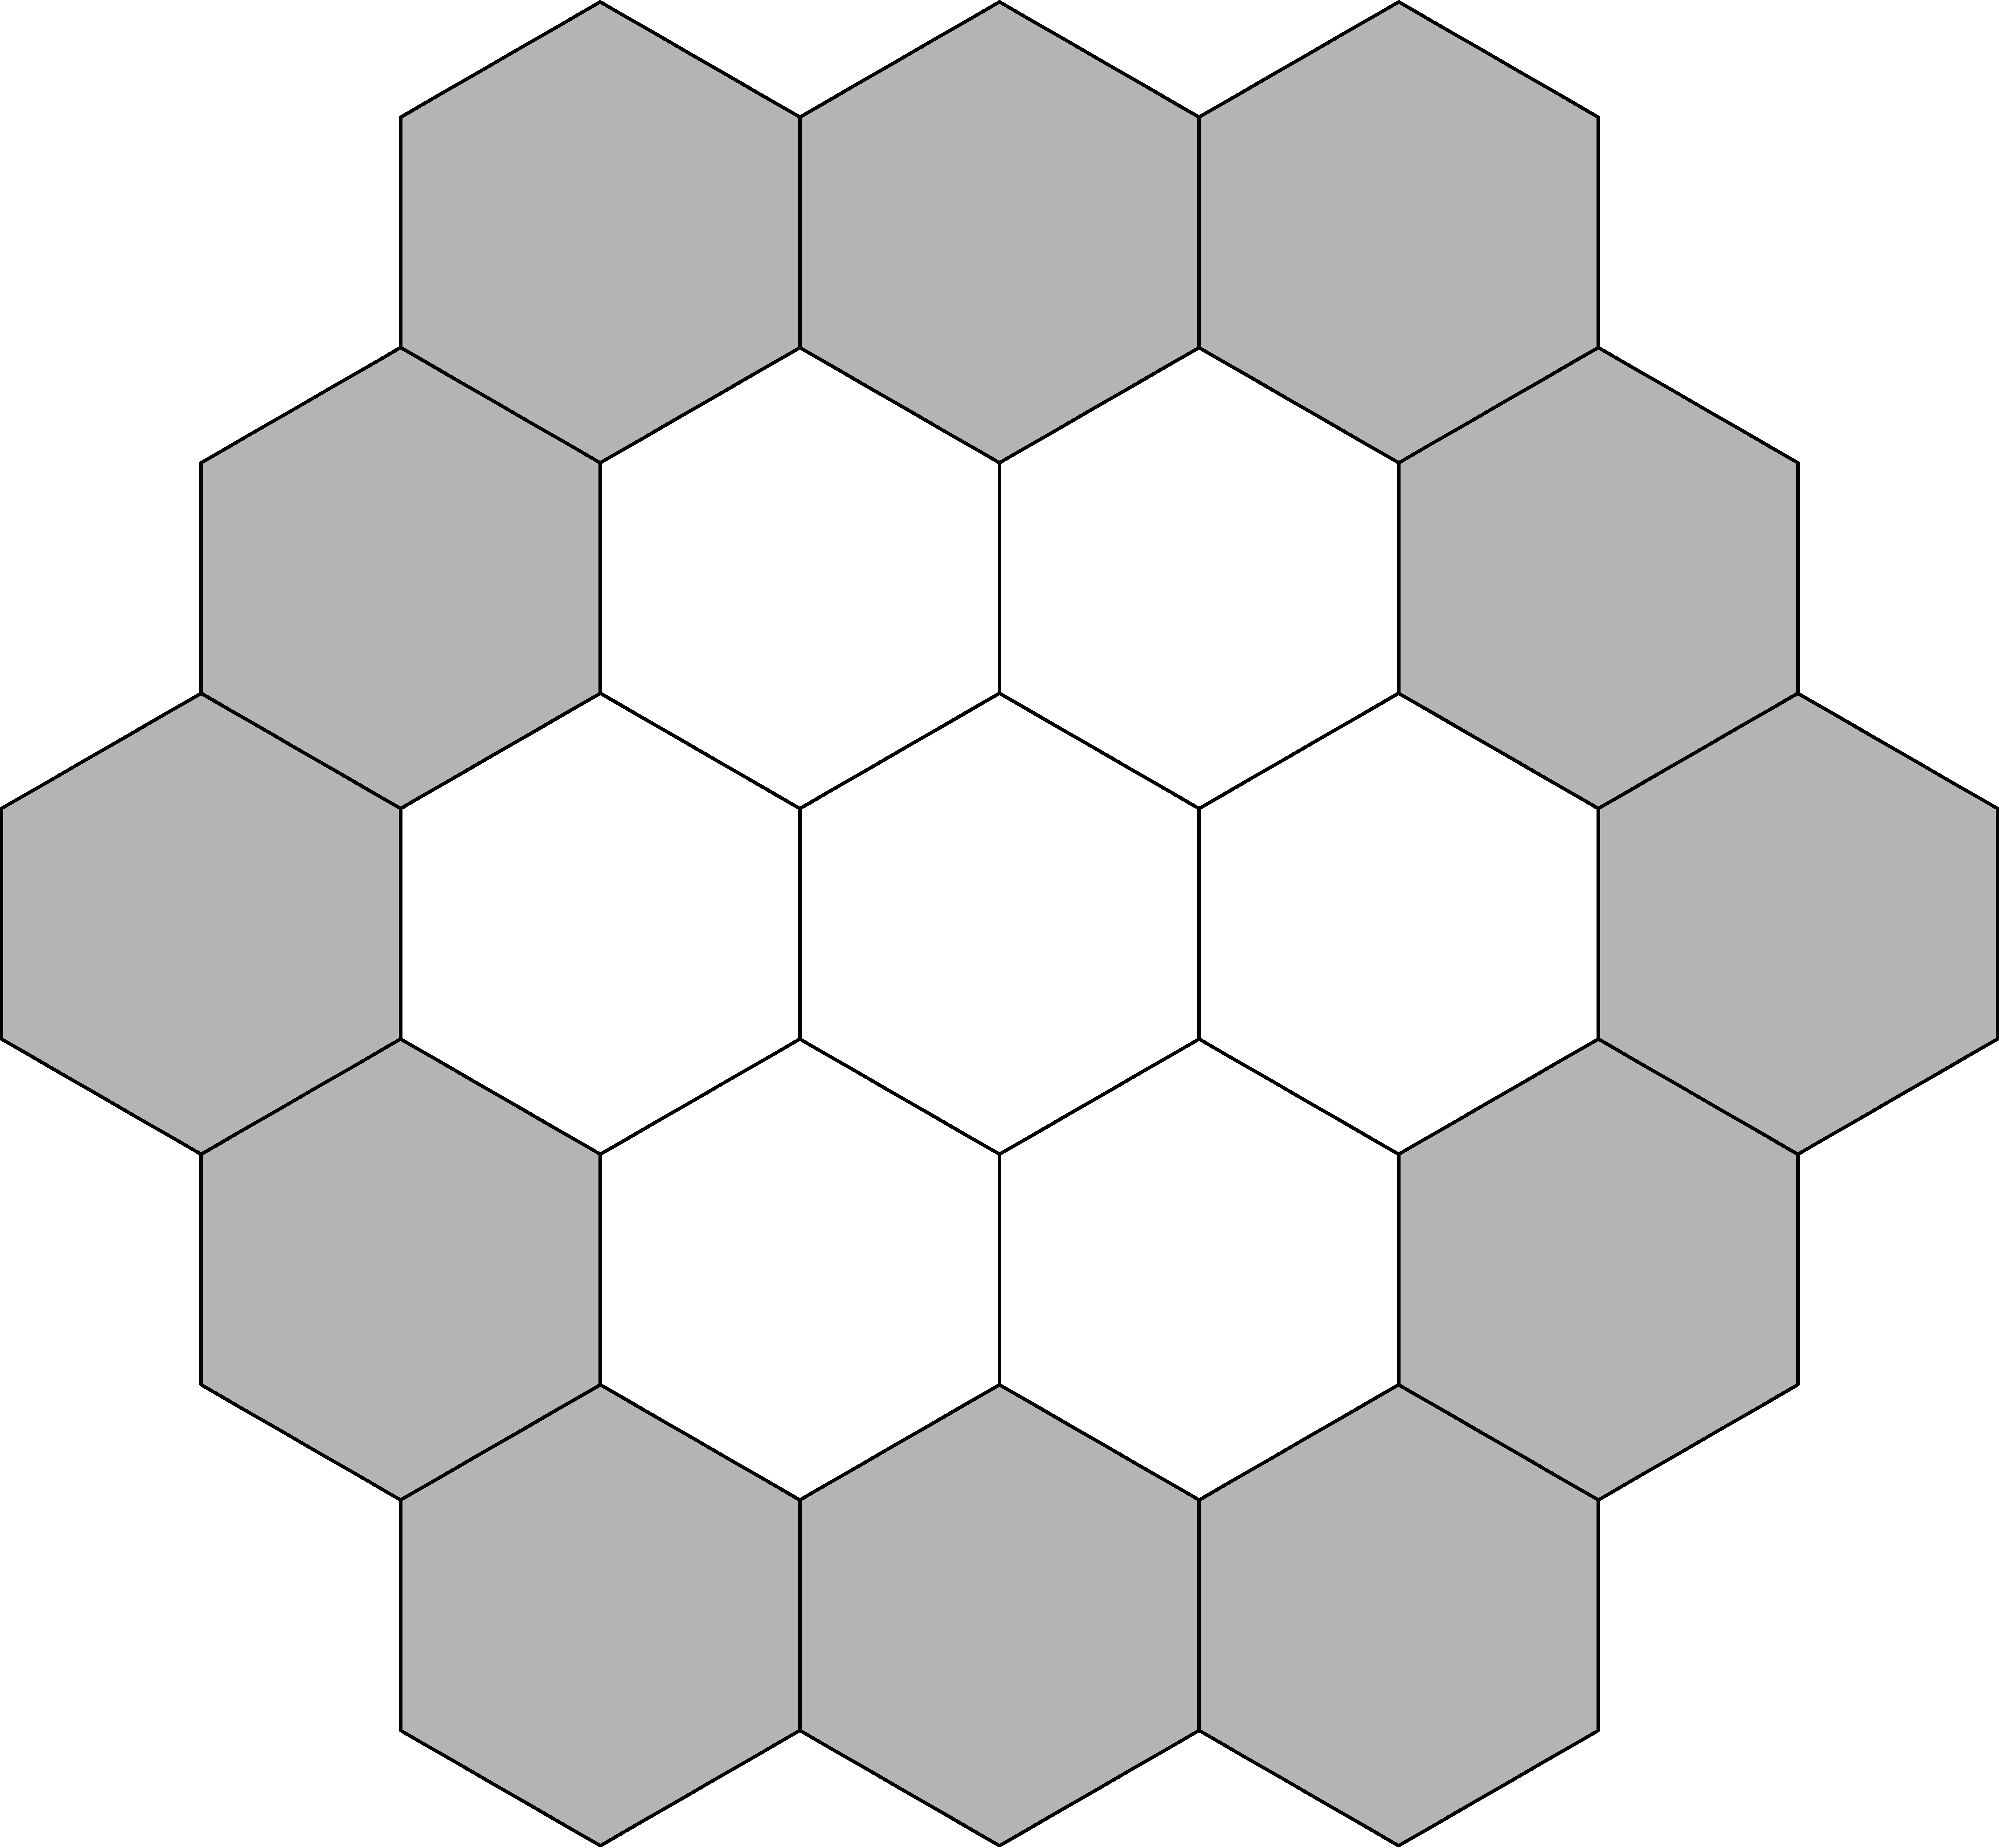
\includegraphics[width=0.4\columnwidth]{./12.simple_threshold_scheduling/img/scenario}
    \caption{The cells in the cluster (white) experience the \gls{oci} generated
    by the interfering cells (shaded).}
    \label{fig:scenario_threshold}
\end{figure}

\reff{fig:scenario_threshold} shows the scenario used in this chapter, where the
white cells form the cluster under study, and the shaded cells represent the out
of cluster interferers.

At each simulation run, 100 \gls{iid} users are randomly placed within each cell
of the cluster, according to a uniform spatial distribution over each cell. Each
of the users has the same antennas as each of the \glspl{bs}, \ie $t=r$, either
2 or 3 in the simulations.

The channel model used is described in \refs{sec:channel_model}.

After all the users are placed in the scenario, they are scheduled for
transmision and immediately after that the rate is calculated for the following
transmission options:

\begin{itemize}
    \item All \glspl{bs} transmit using \gls{su}.
    \item All \glspl{bs} transmit using \gls{bd}.
    \item The transmission strategy is chosen using the algorithm and scheduling
        proposed in this paper.
    \item The same as the previous, but the scheduling is performed based on the
        rates obtained using \gls{bd} instead of the approximation in
        \eqref{eq:bd_frob}.
\end{itemize}

In all cases, the power assignment is done using the scaled water-filling
described in \refss{ssec:scaled_wf}, in order to accomodate the \gls{pbpc}.

\begin{figure}[t]
\centering
    \newgeometry{textwidth=0.7\textwidth}
    \input ./12.simple_threshold_scheduling/img/mean_rate_02x02_100user_bd_tikz.tex
    \restoregeometry
\caption{Mean rate obtained for a 2x2 scenario in the presence of \gls{oci}, 100
users per cell.}
\label{fig:mean_rate_2x2}
\end{figure}

\begin{figure}[t]
\centering
    \newgeometry{textwidth=0.7\textwidth}
    \input ./12.simple_threshold_scheduling/img/mean_rate_03x03_100user_bd_tikz.tex
    \restoregeometry
\caption{Mean rate obtained for a 3x3 scenario in the presence of \gls{oci}, 100
users per cell.}
\label{fig:mean_rate_3x3}
\end{figure}

\reff{fig:mean_rate_2x2} and \reff{fig:mean_rate_3x3} show the mean achievable
rate per user for the transmission options considered, and for two \gls{mimo}
configurations, $t=r=2$ and $t=r=3$ respectively. First thing that can be seen
is how the \gls{oci} severely degrades the performance of \gls{bd}, especially
in the low \gls{snr} regime, where it actually performs worse than not using
coordination at all. The user of the mixed strategy proposed in this work
improves the performance over the whole \gls{snr} range. It is important to note
how the approximation suggested in \eqref{eq:bd_frob} is highly accurate,
compared to using \gls{bd} to calculate the rates for the scheduling algorithm.
And not only is it accurate, but it also is much simpler to implement and much
less computationally expensive
\footnote{As described in \refc{ch:system_model} the \gls{bd} computation
involves two \gls{svd}, which has an overall computational complexity of
$O\left(mn^2\right)$ for a matrix of dimmensions $m \times n$,
\cite{golub2012matrix}. In contrast the computation of Frobenius norm, which
essentially requires the addition of all the elements of a matrix, with a
complexity of $O\left(mn\right)$.}

\begin{figure}[t]
\centering
    \newgeometry{textwidth=0.7\textwidth}
    \input ./12.simple_threshold_scheduling/img/mean_rate_vs_users_02x02_s10_tikz.tex
    \restoregeometry
\caption{Mean rate for a 2x2 scenario as a function of the number of users per cell, for an SNR of 10\,dB.}
\label{fig:mean_rate_vs_users}
\end{figure}

In \reff{fig:mean_rate_vs_users} the mean achievable rate per user is presented as a function of the number of users per cell, for a fixed value of \gls{snr} of
10\,dB. The improvement introduced by the proposed scheme with respect to both
\gls{bd} and \gls{su} increases with the number of users per cell. This is easy
to explain, as the more users there are in each cell, the increased multiuser 
diversity makes it more likely to find the right users to form a group.

It is clear, from the previous results, that the \gls{oci} has a very serious
impact on the performance of \gls{bd}, but this is even more severe when the
fairness of the rates of all users is considered. \reff{fig:cdf_snr10}
represents the \gls{cdf} of the rates obtained with each of the transmission
strategies for a fixed value of \gls{snr} of 10\,dB. It can be seen how the
rates obtained using the mixed strategy are always higher than using each of the
strategies, \gls{bd} or \gls{su}, independently. This difference in favor of the
mixed strategy is even higher for the users with the lowest rates, which
indicates an improvement in the fairness of the system.

\reff{fig:worst_rate} shows the average rate for the 5\,\% worst users. For
these users, \gls{bd} in the presence of \gls{oci} performs poorly, and the use
of the hybrid strategy proposed in this work allows to recover from the loss due
to the \gls{oci}, and to match the performance obtained using \gls{su}.

\begin{figure}[t]
\centering
    \newgeometry{textwidth=0.7\textwidth}
    \input ./12.simple_threshold_scheduling/img/cdf_02x02_s20_100user_bd_tikz.tex
    \restoregeometry
\caption{CDF of the rates obtained in a 2x2 scenario, with an SNR of $10$\,dB.}
\label{fig:cdf_snr10}
\end{figure}

\begin{figure}[t]
\centering
    \newgeometry{textwidth=0.7\textwidth}
    \input ./12.simple_threshold_scheduling/img/mean_rate_005_worst_02x02_100user_bd_tikz.tex
    \restoregeometry
\caption{Mean rate of the 5\% worst users, in a 2x2 scenario in the presence of OCI, 100 users per cell.}
\label{fig:worst_rate}
\end{figure}


% Conclusions
\chapter{Conclusions and Future Work}\label{ch:conclusions_and_future}

% ------------------------------------------------------------------------------
\section{Conclusions} \label{sec:conc}

This work has analyzed the downlink of a clustered cellular network using
cooperation among the \glspl{bs} in the cluster through \gls{bd}. \gls{bd} is
able to eliminate the interference within the cluster, but does not handle the
\gls{oci}. Under these conditions, an analytical expression has been derived for
the mean achievable rate per user, which allows for an analysis of the influence
of different parameters of the system, such as the \gls{snr}, the antenna
configuration, the path-loss, and the cluster size. The derivation requires some
approximations that are used in order to model the \gls{oci}, which is
oversimplified as Gaussian noise, or neglected completely, in other works in the
literature.

Several effects have been observed, some of which have opposing impact on the
mean achievable rate:

\begin{itemize}
   \item Increasing the size of the cluster brings a natural reduction in the
      interference coming from other clusters.
   \item The coordination gain saturates because of the path-loss.
   \item Additionally, the increasing size yields a reduction in the power
      available for each data stream of each user (when the uniform power
      allocation is used) due to the need to coordinate with an increasing
      number of users, some of which may be far away.
\end{itemize}

The most interesting result is that the gain due to the coordination does not
grow unboundedly with the size of the cluster, but there is a limit on the size
of the cluster which, once surpassed, the gain obtained is limited. Recall that
the size of the cluster impacts, negatively, directly on the complexity of the
cooperation processing. It is of interest, hence, to form clusters of reduced
size. The present thesis yields a range of seven to ten cells, for a wide range
of \gls{snr}, and for different antenna configurations.

Apart from the mean achievable rate, also fairness considerations have been
analyzed in the same scenario, with the same \gls{bd} transmission strategy. In
order to do so, the \gls{cdf} of the achievable rate per user is shown to be
very accurately approximated via a Gamma distribution. Also the effects of
several system parameters have been taken into account and their effect on the
fairness of the system studied. In particular, even though an optimal power
allocation enables to increase the mean achievable rate, the fairness is
seriously affected by the power allocation scheme, and a much simpler uniform
power allocation is able to deliver equitable rates among the users.

By comparing the results of \gls{bd} on a scenario such as the one under study
in this thesis, it is clear to see how \gls{bd} and other coordination
techniques are not able to perform as well as expected. That is the reason why,
after analyzing a scenario where the \gls{oci} plays a main role, a simple yet
effective strategy has been proposed in order to overcome the impairments
introduced by the \gls{oci}. The strategy, consisting on a transmission scheme
based on local decisions made by the users of the system, is able to eliminate
the pernicious impact of the \gls{oci} on the performance of coordination
techniques, such as \gls{bd}.

An interesting collateral effect of the decisions being local to the users, is
that it makes the strategy able to adapt to changes in the conditions of the
channel of the users. Additionally, the fairness of the system is also improved,
for the users experiencing the lowest rates are the ones most benefitted from
the strategy proposed.

Finally, the complexity of the method proposed is kept low through the use of a
low complexity user scheduling algorithm that prevents the network from needing
to calculate \gls{svd}, which may be costly, especially as the number of users
per cell increases.

% ------------------------------------------------------------------------------
\section{Future lines of research} \label{sec:future}

The outcome of this thesis is, in a few words, that using clustering is
advantageous if coordination is intended to be used in real world scenarios. And
in this line, the proposal of a simple transmission strategy, with a low
complexity user scheduling algorithm, opens the door for further improvements to
make it an alternative for real applications.

In particular, there is an aspect that requires deeper analysis, and this is the
local decisions made by the users. This decisions are made by comparison of a
metric with a given threshold. In the current work the threshold has been
obtained via simulations, and this seriously reduces its attractiveness for
actual implementations. An interesting future line of work is trying to find a
way to calculate this threshold analytically, or at least not relying on
simulations to obtain it.

During the whole work, the assumptions made, although more or less common in the
literature, may be a bit strong in some circunstances. For instance the most
stringent one is the assumption that the \gls{csi} knowledge is perfect in all
the \glspl{bs}. A study of the influence of having imperfect \gls{csi} would be
a natural extension of the present work. Another imperfection that has not been
considered in this thesis, and that may be of importance when considering
transmitters located in distant locations, is the synchronization among them.

The proposed transmission strategy already alleviates the feedback capacity
required, for users not requesting coordination do not need to feed back the
whole channel matrix. Despite that, beamforming has the inherent need for
sharing user data, and this poses a big burden on the backhaul network. The
study of smart and efficient ways of distributing this information is an
interesting aspect to research.


\appendix

%%%%%%%%%%%%%%%%%%%%%%%%%%%%%%%%%%%%%%%%%%%%%%%%%%%%%%%%%%%%%%%%%%%%%%%%%%%%%%%%
% APPENDICES

\chapter{Derivation of $Z_i$}\label{ch:appendix_a}

Using the change of variable

\begin{equation} \label{eq:change_variable_1}
    v = \frac{u}{\Rcell}
\end{equation}

\noindent
in \eqref{eq:zi_def}, it becomes

\begin{equation} \label{eq:zi_1}
    Z_i = \int\limits_0^1\log\left(\frac{v^{-\gamma}}{\frac{\sigma_i^2}
    {P_{\max}\Rcell^{-\gamma}} + \Meqi\left(\bar{d}_i - v\right)^{\gamma}}
    \right)2v \dee v
\end{equation}

Recall the definition of the \gls{snr} $\rho$ in \eqref{eq:snr_noise}, then

\begin{equation} \label{eq:zi_2}
\begin{aligned}
    Z_i &= \int\limits_0^1\log\left(\frac{v^{-\gamma}}{\frac{1}{\rho} + \Meqi
    \left(\bar{d}_i-v\right)^{-\gamma}}\right)2v \dee v\\
    &= 2 \underbrace{\int\limits_0^1\log\left(\frac{1}{\frac{1}{\rho}+\Meqi
    \left(\bar{d}_i-v\right)^{-\gamma}}\right)v\dee v}_{\mathtt{I}} - 2\gamma
    \underbrace{\int\limits_0^1\log\left(v\right) v\dee v}_{\mathtt{II}}
\end{aligned}
\end{equation}

The term $\mathtt{II}$ in \eqref{eq:zi_2} is evaluated using (2.723) from
\cite{gradshteyn00}, namely

\begin{equation} \label{eq:zi_term2}
    \int v\log\left(v\right)\dee v = v^2\left(\frac{\log\left(v\right)}{2} -
    \frac{1}{4}\right)
\end{equation}

Using the change of variable

\begin{equation} \label{eq:change_variable_2}
    w = \bar{d}_i - v
\end{equation}

\noindent
in the term $\mathtt{I}$ of \eqref{eq:zi_2}, it becomes

\begin{equation} \label{eq:zi_term1}
\begin{aligned}
    \mathtt{(I)} &= -\int\limits_{\bar{d}_i}^{\bar{d}_i -1}
    \log\left(\frac{\rho}{1 + \Meqi\rho w^{-\gamma}}\right)\left(\bar{d}_i - w
    \right)\dee w\\
    &=\underbrace{\int\limits_{\bar{d}_i-1}^{\bar{d}_i}\log\left(\rho\right)
    \left(\bar{d}_i-w\right)\dee w}_{\mathtt{III}} +
    \underbrace{\int\limits_{\bar{d}_i-1}^{\bar{d}_i}\log\left(\frac{1}
    {1 + \Meqi\rho w^{-\gamma}}\right)\left(\bar{d}_i - w\right)\dee w}_
    {\mathtt{IV}}
\end{aligned}
\end{equation}

The term $\mathtt{III}$ of \eqref{eq:zi_term1} is straightforward to calculate

\begin{equation} \label{eq:zi_term3}
    \int\limits_{\bar{d}_i-1}^{\bar{d}_i}\log\left(\rho\right)
    \left(\bar{d}_i-w\right)\dee w = \log\left(\rho\right)
\end{equation}

On the other hand, the term $\mathtt{IV}$ in \eqref{eq:zi_term2} can be computed
using the following result from \cite{Wolfram}

\begin{equation} \label{eq:zi_term4}
\begin{aligned}
    \int\limits_{\bar{d}_i-1}^{\bar{d}_i}\log\left(\frac{1}
    {1 + \Meqi\rho w^{-\gamma}}\right)\left(\bar{d}_i - w\right)\dee w &= w\left[\vphantom{\frac{1}{1}}
    \frac{2\bar{d}_i-w}{2}\log\left(\frac{w^{\gamma}}
    {\Meqi\rho + w^{\gamma}}\right)\right.\\
    &-\bar{d}_i\gamma \hgeo\left(1,\frac{1}{\gamma};\frac{\gamma+1}{\gamma};
    \frac{-w^{\gamma}}{\Meqi\rho}\right)\\
    &+\frac{w\gamma}{4}\hgeo\left(1,\frac{2}{\gamma};\frac{\gamma+2}{\gamma};
    \frac{-w^{\gamma}}{\Meqi\rho}\right)
    \left.\vphantom{\frac{1^2}{1}}\right]
\end{aligned}
\end{equation}

\noindent
where

\begin{equation} \label{eq:hypergeometric}
    \hgeo\left(a,b;c;z\right) = \frac{\Gamma\left(c\right)}{\Gamma\left(b\right)
    \Gamma\left(c - b\right)}\int\limits_0^1\frac{x^{b-1}\left(1-x\right)^
    {c-b-1}}{\left(1-x\right)^a}\dee x
\end{equation}

\noindent
is the hypergeometric function.

Combining the previous, $Z_i$ can be expressed as

\begin{equation} \label{eq:zi_appendix}
\begin{aligned}
    Z_i &= \frac{\gamma}{2} + \log\left(\rho\right) + \bar{d}_i^2\log\left(
    \frac{\bar{d}_i^{\gamma}}{\Meqi \rho + \bar{d}_i^{\gamma}}\right)\\
    &- 2 \bar{d}_i^2\gamma \hgeo \left(1,\frac{1}{\gamma};
    \frac{\gamma+1}{\gamma};\frac{-\bar{d}_i^{\gamma}}{\Meqi\rho +
    \bar{d}_i^{\gamma}}\right)\\
    &+ \frac{\bar{d}_i^2}{2}\gamma \hgeo\left(1, \frac{2}{\gamma};
    \frac{\gamma+2}{\gamma};\frac{-\bar{d}_i^{\gamma}}{\Meqi\rho +
    \bar{d}_i^{\gamma}}\right)\\
    &- \left(\bar{d}_i^2-1\right)\log\left(
    \frac{\left(\bar{d}_i-1\right)^{\gamma}}
    {\Meqi\rho+\left(\bar{d}_i - 1\right)^{\gamma}}\right)\\
    &+ 2\bar{d}_i\left(\bar{d}_i - 1\right)\gamma\hgeo\left(1,\frac{1}{\gamma};
    \frac{\gamma + 1}{\gamma};\frac{-\left(\bar{d}_i-1\right)^{\gamma}}
    {\Meqi\rho}\right)\\
    &- \frac{\left(\bar{d}_i-1\right)^2}{2}\gamma\hgeo\left(1,\frac{2}{\gamma};
    \frac{\gamma + 2}{\gamma};\frac{-\left(\bar{d}_i-1\right)^{\gamma}}
    {\Meqi\rho}\right)
\end{aligned}
\end{equation}



\chapter{Characterization of $\thetath$}
\label{ch:appendix_b}

In this chapter, a brief analysis of the threshold $\thetath$ is
offered in order to show its dependence on some of the scenario parameters, for
instance:

\begin{itemize}
    \item Number of antennas of the \gls{mimo} configuration.
    \item \gls{snr} of the system.
    \item Cluster size.
    \item Path loss exponent $\gamma$.
\end{itemize}

Figures \ref{fig:th_exp_tiers} through \ref{fig:th_snr_ant} show this dependence
for a series of combinations of parameters.

First, \reff{fig:th_snr_tiers} and \reff{fig:th_snr_ant} show how the threshold
is consistently independent from the \gls{snr}, except for very low values of
it.

For increasing values of the path loss exponent, the threshold increases as
well, as it can be seen in \reff{fig:th_exp_tiers} and \reff{fig:th_exp_ant}. A
higher path loss exponent translates into a lower level of interference between
adjacent cells, in which case coordination may not help at all, so each \gls{bs}
better serves its own users independently. This is the reason for a higher
threshold, which implies that less users will select \gls{bd} as their preferred
transmission strategy.

Another interesting characteristic that is clear in \reff{fig:th_exp_ant} and
\reff{fig:th_snr_ant} is how the number of antennas plays no role in the
threshold.

These two suggestions mean the advantages that \gls{mimo} has to offer have
no influence on the value of the $\thetath$, and it should depend mainly on the
propagation characteristics of the channel.

This claim can be supported by \reff{fig:th_exp_tiers} and
\reff{fig:th_snr_tiers}, which show the behavior of the threshold with the
cluster size, and by the already mentioned dependence on the path loss exponent.
Cluster size is represented by the number of hexagonal tiers that form the
cluster, so that 1 tiers is a 7 cells cluster, 2 tiers is a 19 cells cluster,
and 3 tiers corresponds to a 37 cells cluster.

Similarly to what happened with the path loss exponent, a bigger cluster means
that cells within a cluster may be too far away from some users in the cluster,
who may not benefit much from coordination. As observed with the path loss
exponent $\gamma$, reducing the level of influence among the cells in the
cluster increases the value of the threshold, in this case when the cluster
considered grows in size. Again, this higher value of $\thetath$ means that more
users will select \gls{su} as their transmission strategy.

\begin{figure}[t]
	\centering
	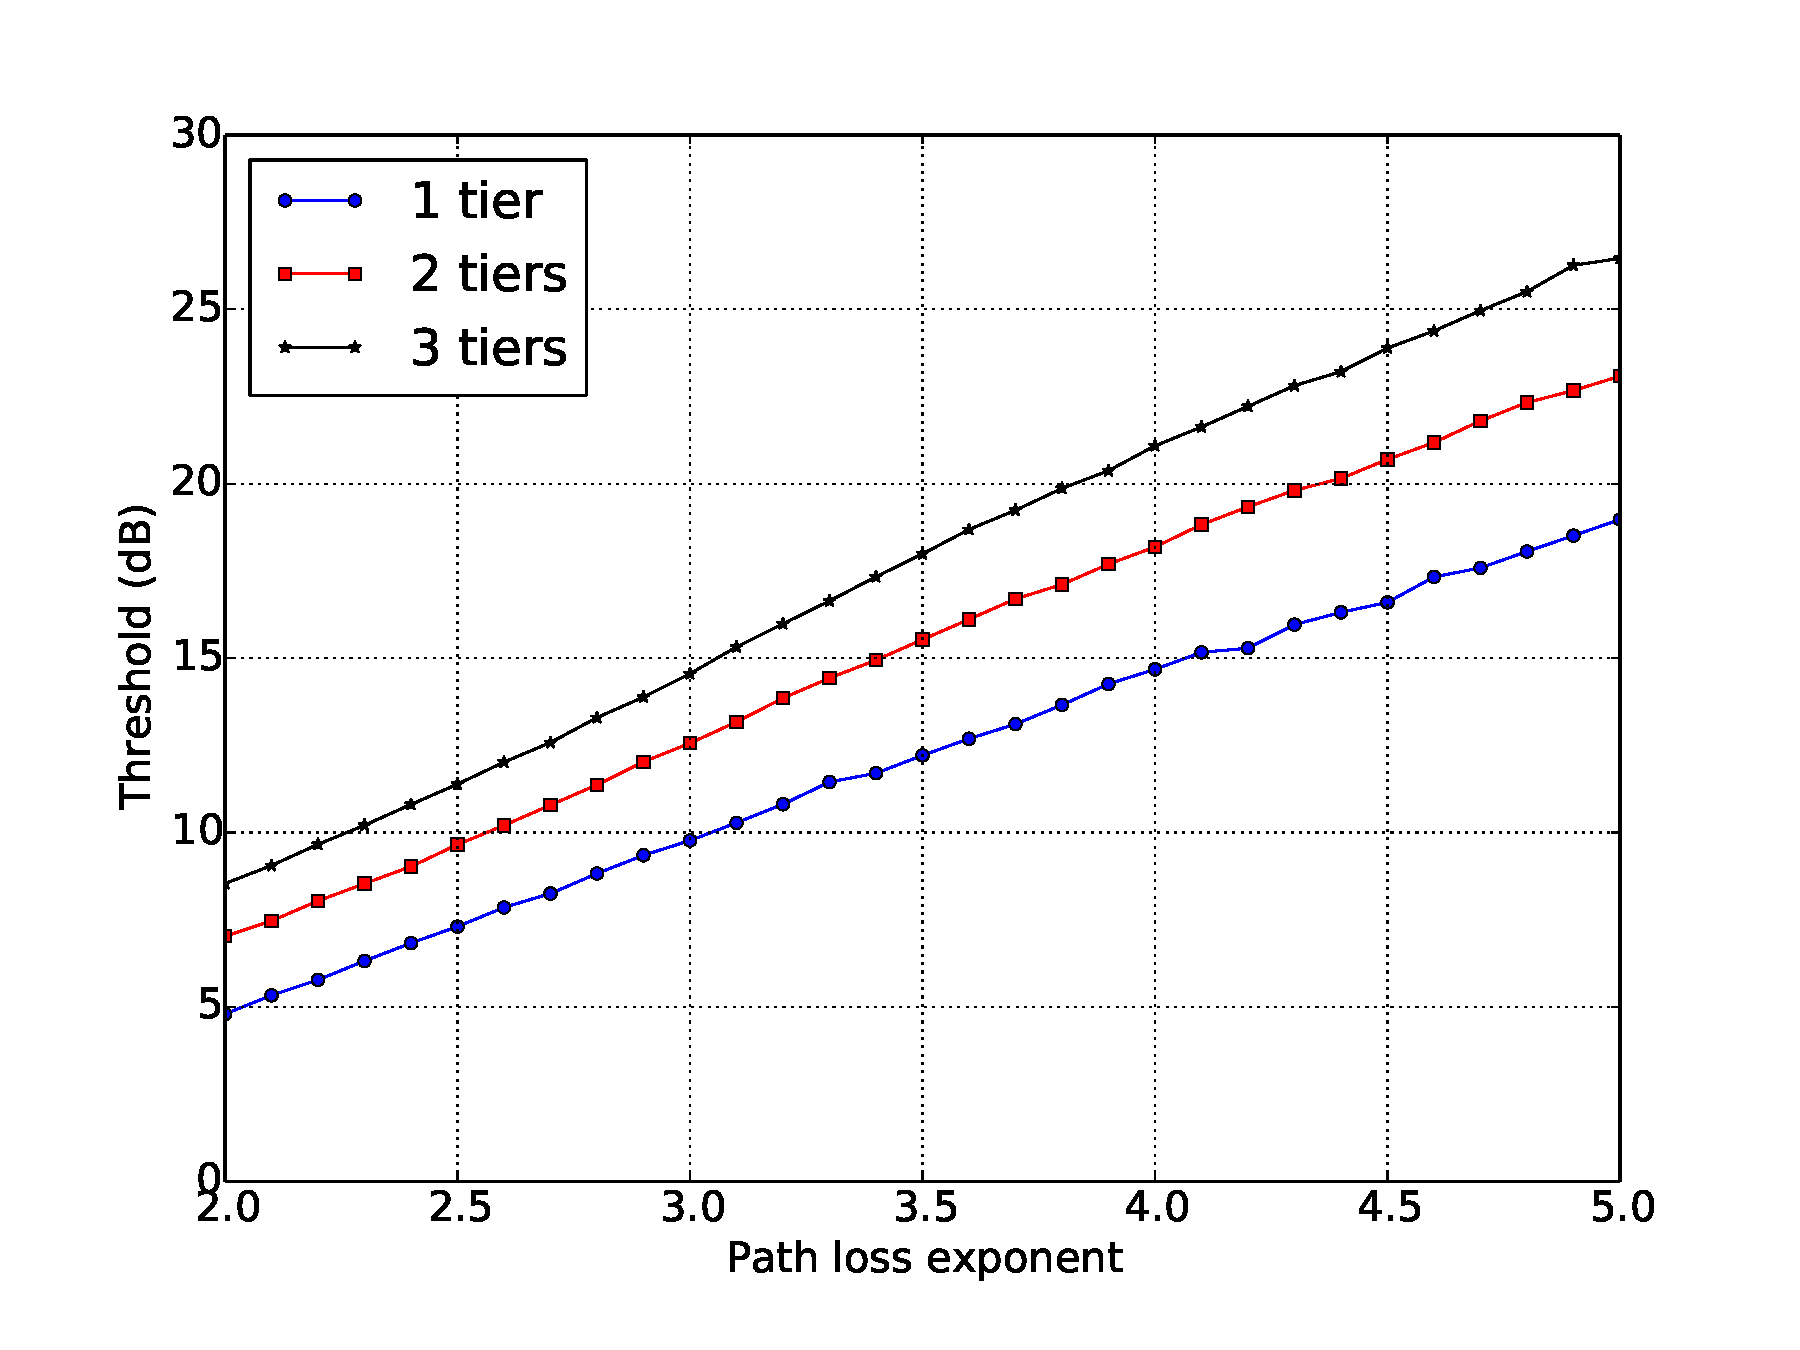
\includegraphics[width=0.75\columnwidth]{./21.appendices/img/threshold_exp_tiers_02x02_s+0015_r1300}
	\caption{Threshold as a function of the path loss exponent, for different
    cluster sizes, for an \gls{snr} of $15$\,dB.}
	\label{fig:th_exp_tiers}
\end{figure}

\begin{figure}[t]
	\centering
	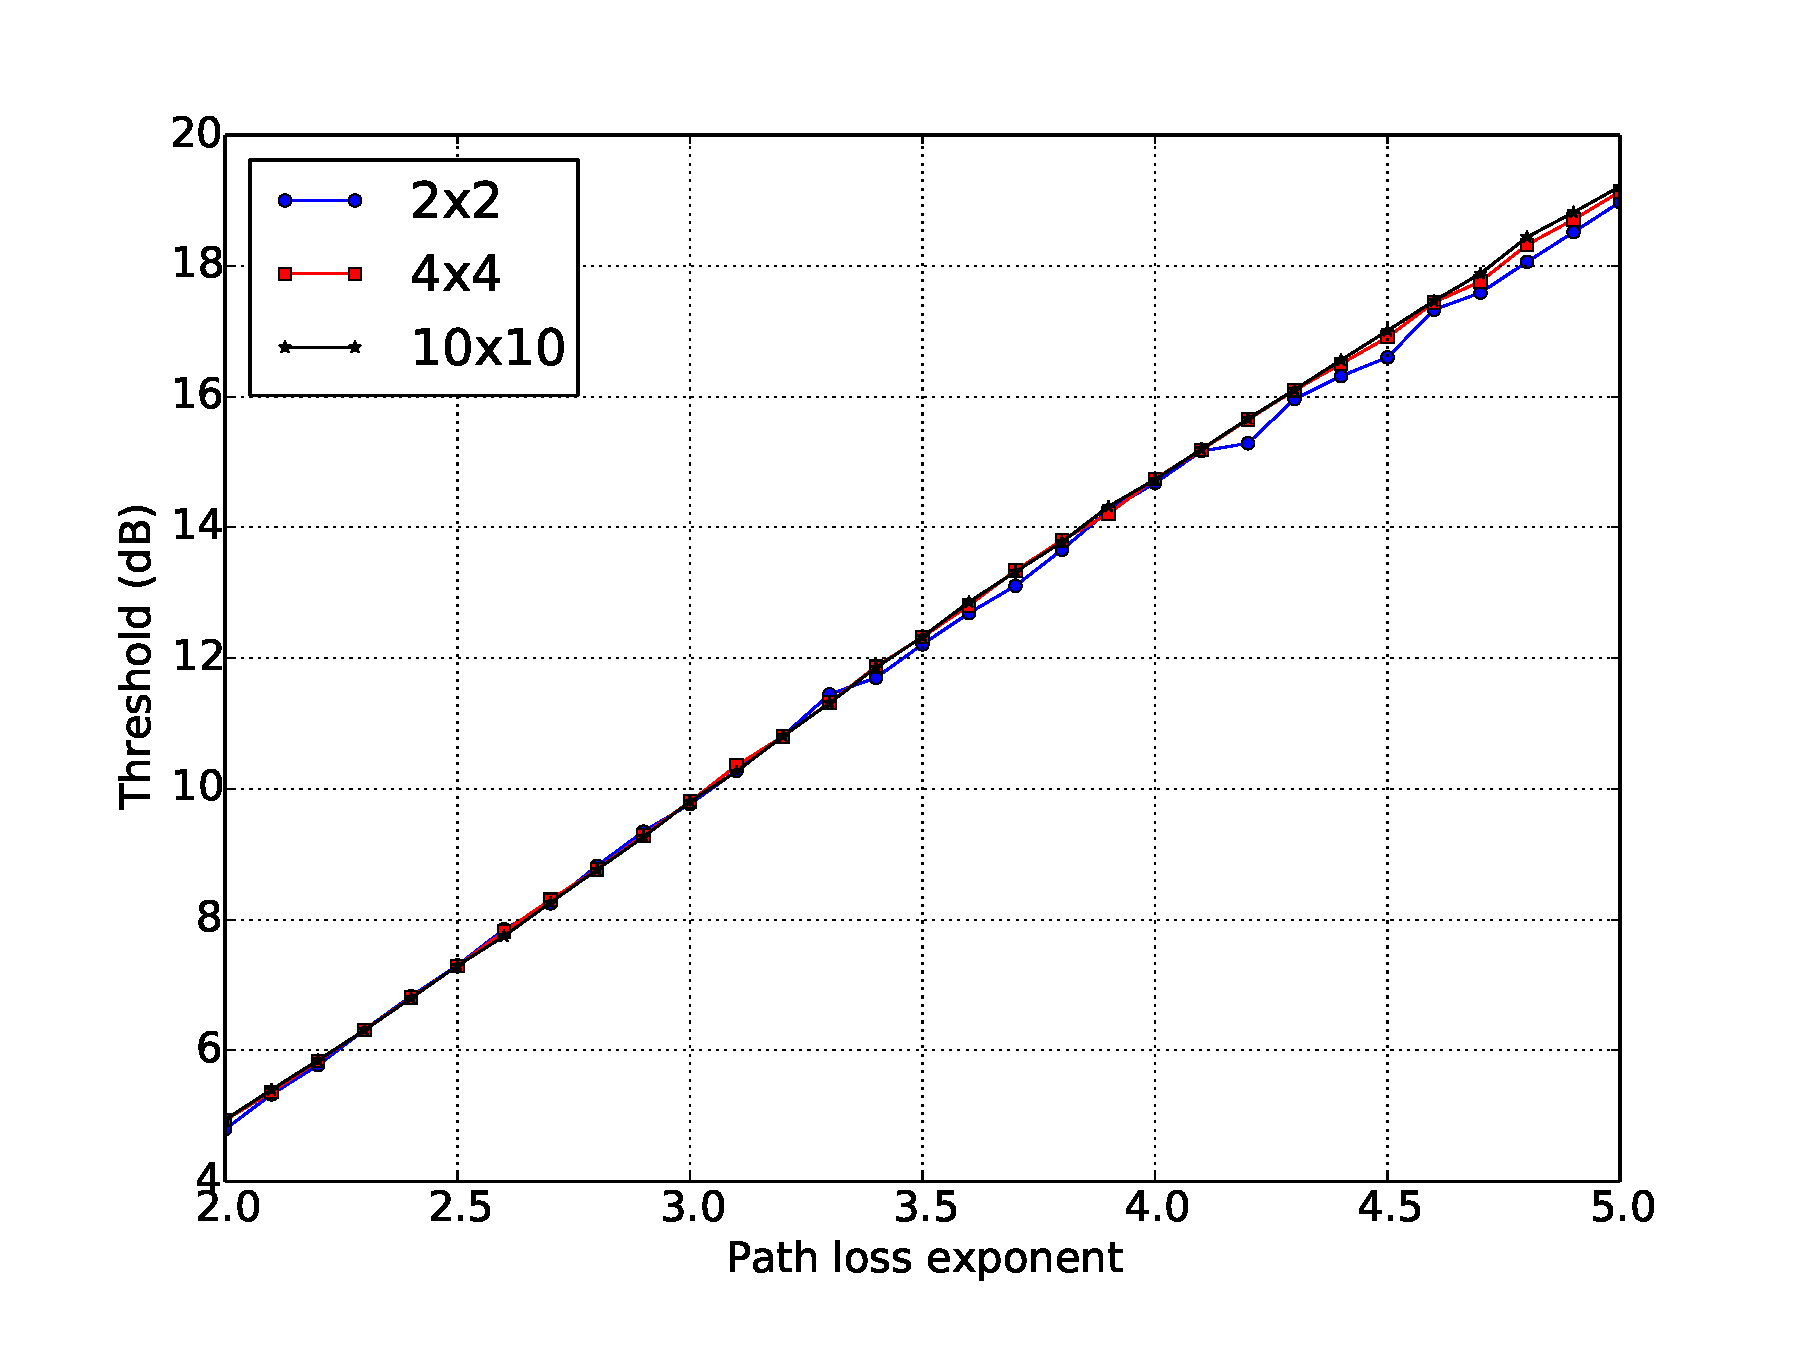
\includegraphics[width=0.75\columnwidth]{./21.appendices/img/threshold_exp_anten_02x02_t02_i01_r1300}
	\caption{Threshold as a function of the path loss exponent, for different
    \gls{mimo} configurations, for an \gls{snr} of $15$\,dB.}
	\label{fig:th_exp_ant}
\end{figure}

\begin{figure}[t]
	\centering
	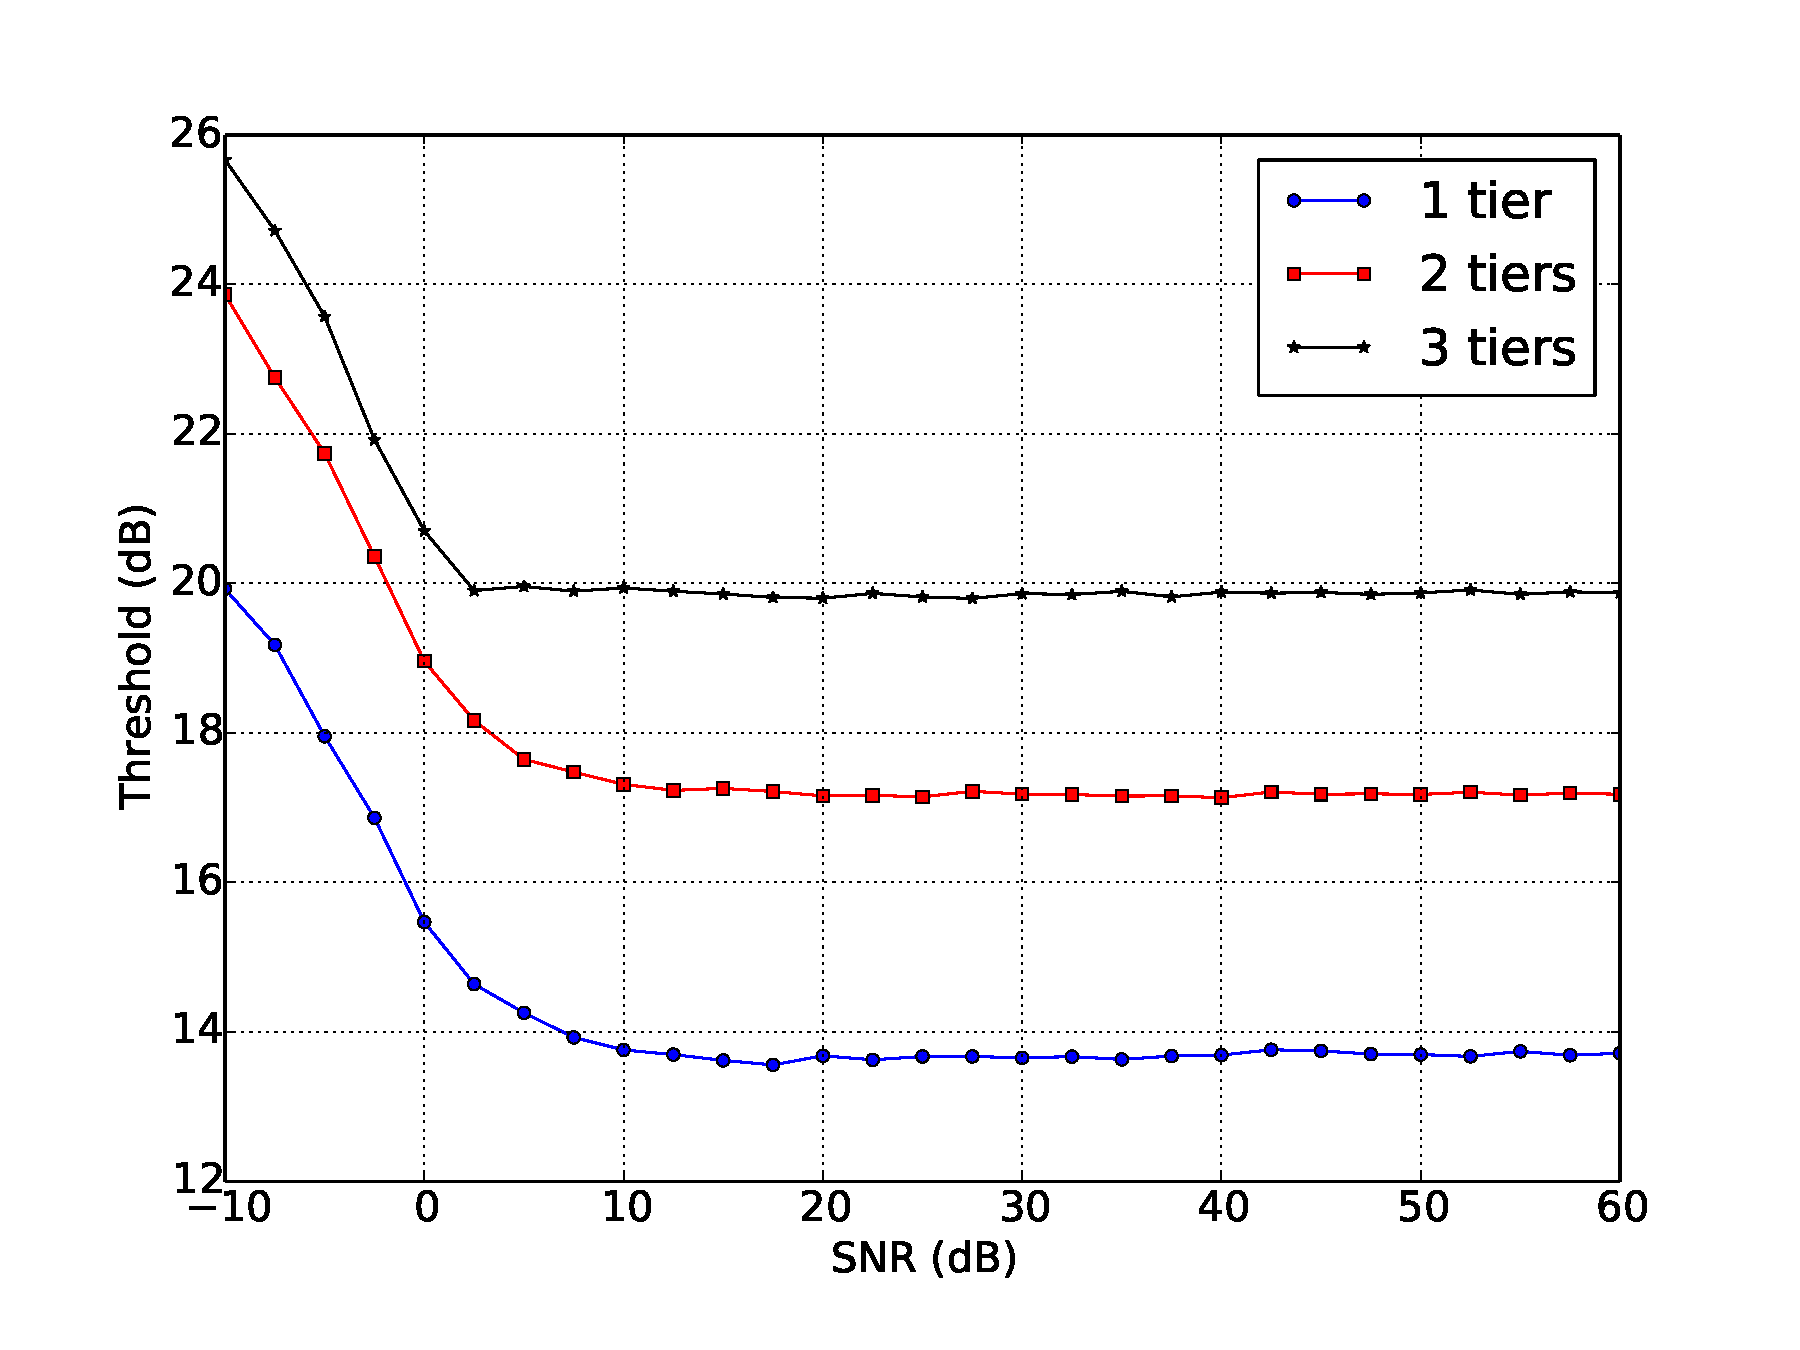
\includegraphics[width=0.75\columnwidth]{./21.appendices/img/threshold_snr_tiers_02x02_c02_r1300}
    \caption{Threshold as a function of the \gls{snr}, for different cluster
    sizes, for $\gamma = 3.8$.}
	\label{fig:th_snr_tiers}
\end{figure}

\begin{figure}[t]
	\centering
	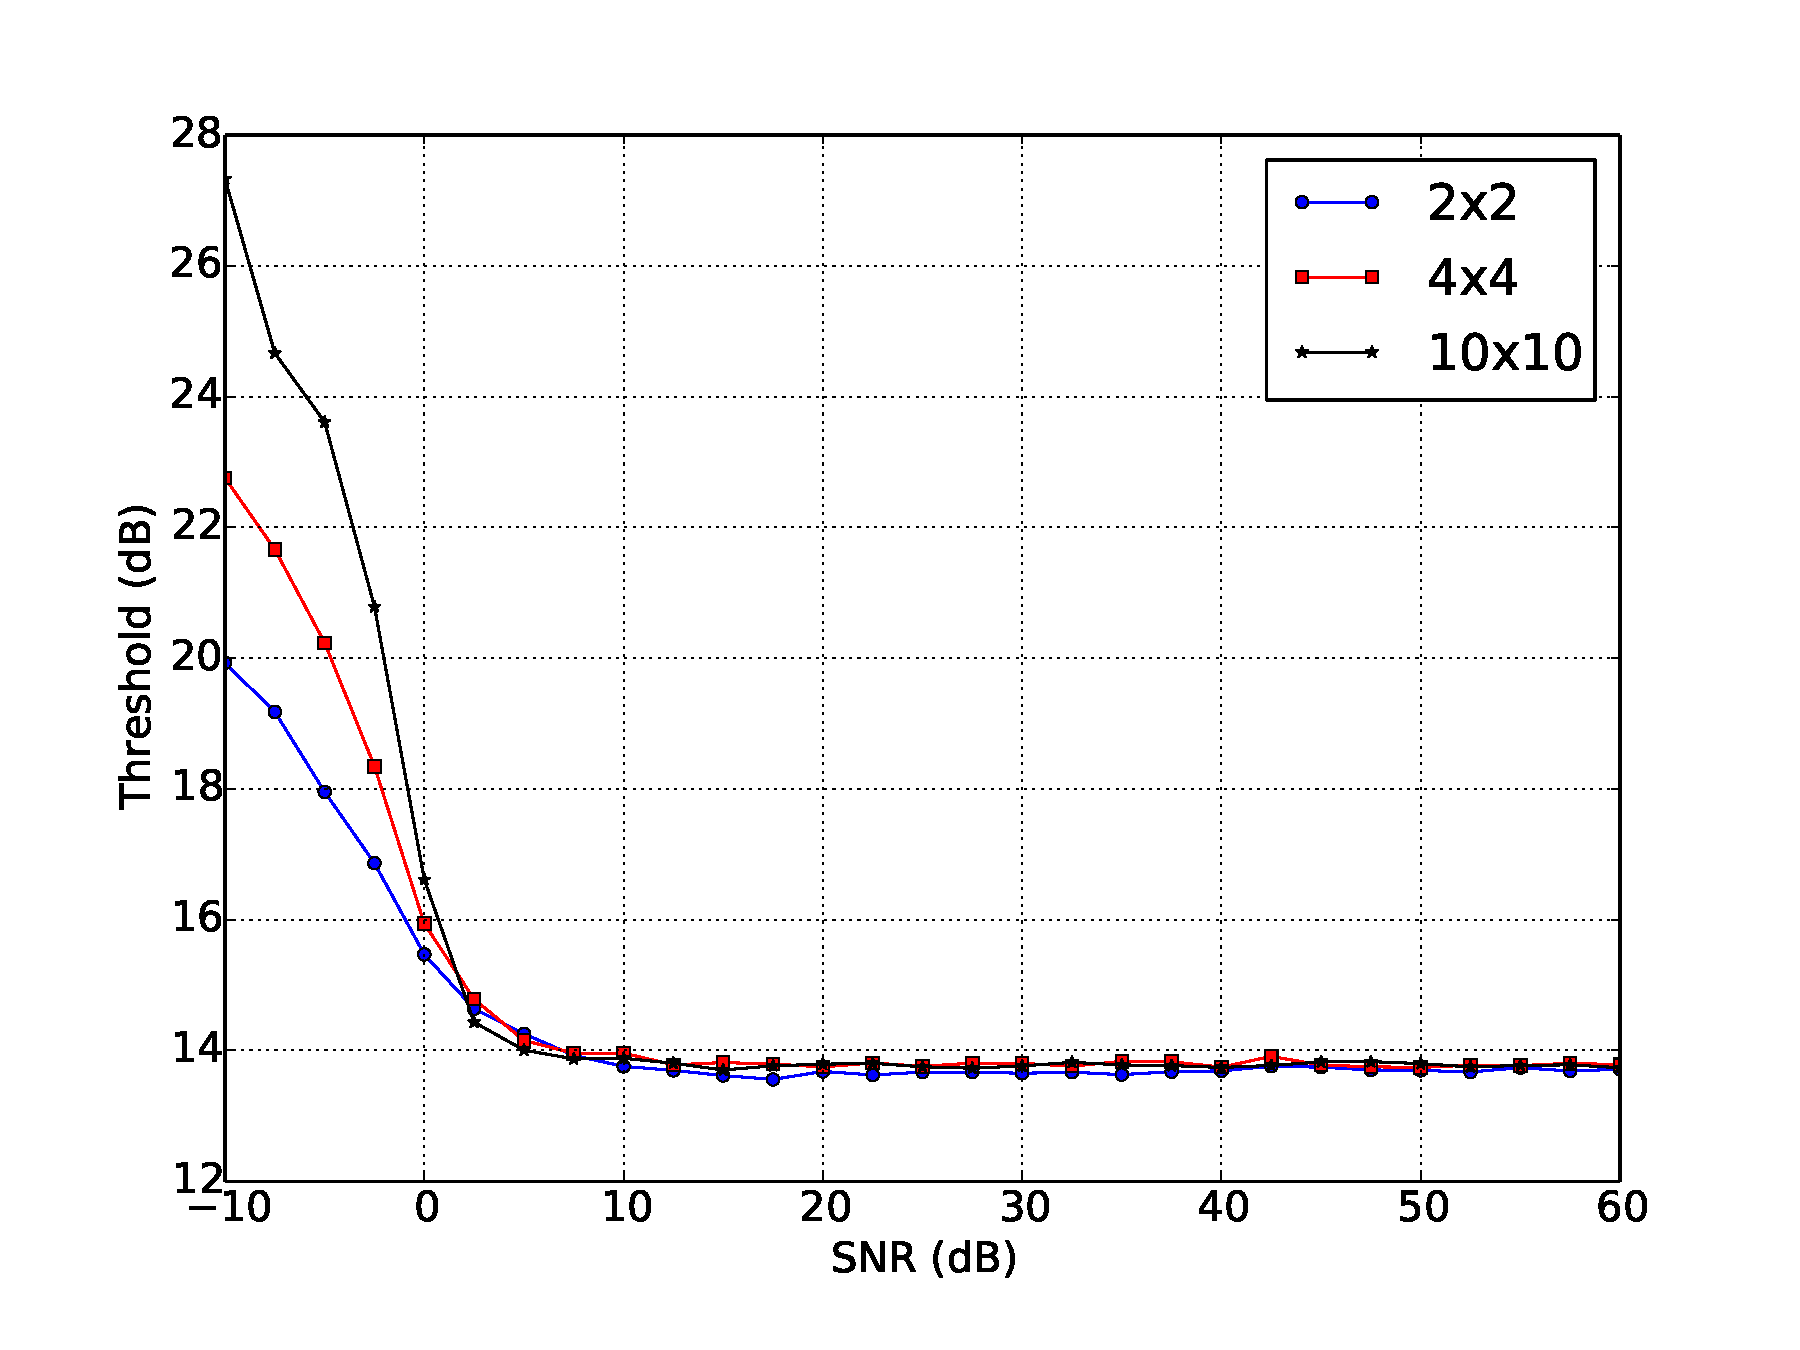
\includegraphics[width=0.75\columnwidth]{./21.appendices/img/threshold_snr_anten_02x02_t02_i01_r1300}
    \caption{Threshold as a function of the \gls{snr}, for different \gls{mimo}
    configurations, for $\gamma = 3.8$.}
	\label{fig:th_snr_ant}
\end{figure}



%%%%%%%%%%%%%%%%%%%%%%%%%%%%%%%%%%%%%%%%%%%%%%%%%%%%%%%%%%%%%%%%%%%%%%%%%%%%%%%%
% REFERENCES

\printbibliography[heading=bibintoc]

\end{document}
